%%%%%%%%%%%%%%%%%%%%%%%%%%%%%%%%%%%%%%%%%%%%%%%%%%%%%%%%%%%%%%%%%%%%%%
% njuthesis 示例模板 v1.4.1 2024-04-19
% https://github.com/nju-lug/NJUThesis
%
% 贡献者
% Yu XIONG @atxy-blip   Yichen ZHAO @FengChendian
% Song GAO @myandeg     Chang MA @glatavento
% Yilun SUN @HermitSun  Yinfeng LIN @linyinfeng
% Yukai Chou @Muzimuzhi
%
% 许可证
% LaTeX Project Public License(版本 1.3c 或更高)
%%%%%%%%%%%%%%%%%%%%%%%%%%%%%%%%%%%%%%%%%%%%%%%%%%%%%%%%%%%%%%%%%%%%%%

%---------------------------------------------------------------------
% 一些提升使用体验的小技巧:
%   1. 请务必使用 UTF-8 编码编写和保存本文档
%   2. 请务必使用 XeLaTeX 或 LuaLaTeX 引擎进行编译
%   3. 不保证接口稳定,写作前一定要留意版本号
%   4. 以百分号(%)开头的内容为注释,可以随意删除
%---------------------------------------------------------------------

%---------------------------------------------------------------------
% 请先阅读使用手册:
% http://mirrors.ctan.org/macros/unicodetex/latex/njuthesis/njuthesis.pdf
%---------------------------------------------------------------------


\documentclass[
    % 模板选项(注意右端逗号):
    %
    % type = bachelor|master|doctor|postdoc, % 文档类型,默认为本科生
    % degree = academic|professional,        % 学位类型,默认为学术型
    %
    % nl-cover,   % 是否需要国家图书馆封面,默认关闭
    decl-page,  % 是否需要诚信承诺书或原创性声明,默认关闭
    %
    %   页面模式,详见手册说明
    % draft,                  % 开启草稿模式
    % anonymous,              % 开启盲审模式
    % minimal,                % 开启最小化模式
    %
    %   单双面模式,默认为适合印刷的双面模式
    % oneside,                % 单面模式,无空白页
    % twoside,                % 双面模式,每一章从奇数页开始
    %
    %   字体设置,不填写则自动调用系统预装字体,详见手册
    % fontset = win|mac|macoffice|fandol|none,
    type=master,
    degree = professional,
  ]{njuthesis}

% 模板选项设置,包括个人信息、外观样式等
% 较为冗长且一般不需要反复修改,我们把它放在单独的文件里
% njuthesis 参数设置文件 v1.4.1 2024-04-19

% 一些提醒:
%   1. \njusetup 内部千万不要有空行
%   2. 使用英文半角逗号(,)分隔选项
%   3. 等于号(=)两侧的空格会被忽略
%       3.1. 为避免歧义,请用花括号({})包裹内容
%   4. 本科生无需填写的项目已被特别标注
%   5. 可以尽情删除本注释

% info 类用于录入个人信息
%   带*号的为对应英文字段
\njusetup[info]{
    title = {面向模型推理场景的\\云边协同调度技术研究},
    % 中文题目
    % 直接填写标题就是自动换行
    % 可以使用换行控制符(\\)手动指定换行位置
    %
    title* = {Research on Cloud-Edge Collaborative Scheduling for Model Inference Scenarios},
    % 英文题目
    %
    author = {蒋一杰},
    % 作者姓名
    %
    author* = {Yijie Jiang},
    % 作者英文姓名
    % 一般使用拼音
    %
    keywords = {云边协同, 模型推理, 动态资源调度, KubeEdge, Akka},
    % 中文关键词列表
    % 使用英文半角逗号(,)分隔
    %
    keywords* = {cloud-edge collaborative, model inference, dynamic resource scheduling, KubeEdge, Akka},
    % 英文关键词
    % 使用英文半角逗号(,)分隔
    %
    grade = {2023},
    % 年级
    %
    student-id = {522023320072},
    % 学号或工号
    % 研究生请斟酌大小写字母格式
    % 本模板并不会自动更正大小写
    %
    department = {软件学院},
    department* = {The Software Institute},
    % 院系
    %
    major = {电子信息(软件工程领域)},
    major* = {Software Engineering},
    % 专业
    %
    % major = {封面专业,摘要专业},
    % 研究生专业型学位可能遇到两处内容不一致的情况
    %
    supervisor = {马晓星教授},
    supervisor*= {Professor~Xiaoxing Ma},
    % 导师全称
    % 使用英文半角逗号(,)分隔中文姓名和职称
    %
    supervisor-ii = {曹春教授},
    supervisor-ii* = {Professor~Chun Cao},
    % 第二导师全称
    % 如果确实没有第二导师,不填写即可
    %
    submit-date = {2025-05-21},
    % 提交日期
    % 格式为 yyyy-mm-dd
    % 不填就是编译当天日期
    %
    %
    % 以下均为研究生项
    %
    % degree = {工程硕士},
    % degree* = {Master of Engineering},
    % 覆盖默认学位名称
    %
    field = {软件工程},
    field* = {Software Engineering},
    % 研究领域
    %
    chairman = {王林章~教授},
    % 答辩委员会主席
    % 推荐使用波浪号(~)分隔姓名和职称
    %
    reviewer = {
        % 徐锋~教授,
        % 余萍~副教授
    },
    %
    % 答辩委员会成员
    % 一般为四名,使用英文半角逗号(,)分隔
    %
    clc = {TP311.5},
    % 中国图书分类号
    %
    udc = {004.41},
    % 国际图书分类号
    %
    secret-level = {公开},
    % 密级
    %
    defend-date = {2025-05-21},
    % 答辩日期
    % 格式为 yyyy-mm-dd
    % 不填就是编译当天日期
    %
    email = {522023320072@smail.nju.edu.cn},
    % 电子邮箱地址
    % 只用于出版授权书
    %
    %
    % 以下用于国家图书馆封面
    confer-date = {2025-06-15},
    % 学位授予日期
    %
    bottom-date = {2025-06-15},
    % 封面底部日期
    %
    supervisor-contact = {
        南京大学~
        江苏省南京市栖霞区仙林大道163号
    }
    % 导师联系方式
}

% bib 类用于参考文献设置
\njusetup[bib]{
    % style = numeric|author-year,
    % 参考文献样式
    % 默认为顺序编码制(numeric)
    % 可选著者-出版年制(author-year)
    %
    resource = {njuthesis.bib},
    % 参考文献数据源
    % 需要带扩展名的完整文件名
    % 可使用逗号分隔多个文件
    % 此条等效于 \addbibresource 命令
    %
    % option = {
        % doi    = false,
        % isbn   = false,
        % url    = false,
        % eprint = false,
        % 关闭部分无用文献信息
        %
        % refsection = chapter,
        % 将参考文献表置于每章后
        %
        % gbnamefmt = lowercase
        % 使用仅首字母大写的姓名
    %   }
    % 额外的 biblatex 宏包选项
}

% image 类用于载入外置的图片
\njusetup[image]{
    % path = {{./figure/}{./image/}},
    % 图片搜索路径
    %
    % nju-emblem = {nju-emblem},
    % nju-name = {nju-name},
    % 校徽和校名图片路径
    % 建议使用 PDF 格式的矢量图
    % 使用外置图片有助于减少编译时间
    % 空置时会自动使用 njuvisual 宏包绘制
    %
    nju-emblem = {nju-emblem-purple},
    nju-name = {nju-name-purple},
    % 替换为紫色版本
    % 这个选项只能填写一次
    % 切换时要注释掉上方的黑色版本
}

% abstract 类用于设置摘要样式
\njusetup[abstract]{
    toc-entry = false,
    % 摘要是否显示在目录条目中
    %
    % underline = false,
    % 研究生英文摘要页条目内容是否添加下划线
    %
    % title-style = strict|centered|natural
    title-style = natural
    % 研究生摘要标题样式,详见手册
}

% 目录自身是否显示在目录条目中
\njusetup{
    tableofcontents/toc-entry = false,
    % 关闭本项相当于同时关闭三个选项
    %
    % listoffigures/toc-entry   = false,
    % listoftables/toc-entry    = false
}

% 为目录中的章标题添加引导线
\njusetup[tableofcontents/dotline]{chapter}

% math 类用于设置数学符号样式,功能详见手册
\njusetup[math]{
    % style              = TeX|ISO|GB,
    % 整体风格,缺省值为国标(GB)
    % 相当于自动设置以下若干项
    %
    % integral           = upright|slanted,
    % integral-limits    = true|false,
    % less-than-or-equal = slanted|horizontal,
    % math-ellipsis      = centered|lower,
    % partial            = upright|italic,
    % real-part          = roman|fraktur,
    % vector             = boldfont|arrow,
    % uppercase-greek    = upright|italic
}

% theorem 类用于设置定理类环境样式,功能详见手册
\njusetup[theorem]{
    % define,
    % 默认创建内置的七种定理环境
    %
    % style         = remark,
    % header-font   = \sffamily \bfseries,
    % body-font     = \normalfont,
    % qed-symbol    = \ensuremath { \male },
    % counter       = section,
    % share-counter = true,
    % type          = {...}
    % 以上设置项在重新调用 theorem/define 后生效
}

% footnote 类用于设置脚注样式,功能详见手册
\njusetup[footnote]{
  % style = pifont|circled,
  % 使用圈码编号
  %
  % hang = false,
  % 不使用悬挂缩进
}

% 页眉页脚内容设置
\njusetup{
  % header/content = {
  %     {OR}{\thepage},{OL}{\rightmark},
  %     {EL}{\thepage},{ER}{\leftmark}
  %   },
  % 页眉设置,详见手册
  % 奇数页页眉:左侧章名,右侧页码
  % 偶数页页眉:左侧页码,右侧节名
  %
  % footer/content = {}
}

% 页眉页脚的字体样式
% \njusetformat{header}{\small\kaishu}
% \njusetformat{footer}{}

% 在盲审模式下隐藏学校信息
% \njusetup{anonymous-mode/no-nju}

% 一些灵活调整
% \njusetname{type}{本科毕业设计}                 % 我做的是毕业设计
% \njusetname{notation}{术语表}                   % 更改符号表名称
% \njusetlength{crulewd}{240pt}                   % 加长封面页下划线
% \njusetformat{tabular}{\zihao{-4}\bfseries}     % 修改表格环境的字号
% \EditInstance{nju}{u/cover/emblem-img}{align=l} % 左对齐的本科生封面校徽

% \usepackage{graphicx}
\usepackage{float}
% 自行载入所需宏包
\usepackage{subcaption} % 嵌套小幅图像,比 subfig 和 subfigure 更新更好
% \usepackage{siunitx} % 标准单位符号
% \usepackage{physics} % 物理百宝箱
% \usepackage[version=4]{mhchem} % 绘制分子式
\usepackage{listings} % 展示代码
\usepackage{algorithm,algorithmic} % 展示算法伪代码

% 在导言区随意定制所需命令
% \DeclareMathOperator{\spn}{span}
% \NewDocumentCommand\mathbi{m}{\textbf{\em #1}}

% 开始编写论文
\begin{document}

%---------------------------------------------------------------------
%	封面、摘要、前言和目录
%---------------------------------------------------------------------

% 生成封面页
\maketitle

% 模板默认使用 \flushbottom,即底部平齐
% 效果更好,但可能出现 underfull \vbox 信息
% 以下命令用于抑制这些信息
\raggedbottom

\begin{abstract}
  中文摘要
\end{abstract}

\begin{abstract*}
  English abstract
\end{abstract*}

% 生成目录
\tableofcontents
% 生成图片清单
% \listoffigures
% 生成表格清单
% \listoftables

%---------------------------------------------------------------------
%	正文部分
%---------------------------------------------------------------------
\mainmatter

% 符号表
% 语法与 description 环境一致
% 两个可选参数依次为说明区域宽度、符号区域宽度
% 带星号的符号表(notation*)不会插入目录
% \begin{notation}[10cm]
%   \item[DFT] 密度泛函理论 (Density functional theory)
%   \item[DMRG] 密度矩阵重正化群 (Density-Matrix Reformation-Group)
% \end{notation}

% 建议将论文内容拆分为多个文件
% 即新建一个 chapters 文件夹
% 把每一章的内容单独放入一个 .tex 文件
% 然后在这里用 \include 导入,例如
%   \include{chapters/introduction}
%   \include{chapters/environments}


\chapter{绪论}

\section{研究背景}

近年来,随着物联网(Internet of Things, IoT)和人工智能(Artificial Intelligence, AI)等技术的迅猛发展,网络边缘设备的数量急剧增加,数据规模持续扩大,进而带来了巨大的计算需求\cite{verma2017survey}。在这些需求中,深度学习在智能工业\cite{yan2017industrial,zhang2017self,peres2018idarts,mohamed2019leveraging}、城市交通\cite{jia2017edge,mohamed2017smartcityware,mallapuram2017smart,dalla2017using}、智慧家居\cite{savio2018smart,krejcar2020technology,黄倩怡2020智能家居中的边缘计算}等领域中发挥着至关重要的作用。云计算可将云端服务器的强大算力赋能给性能有限的终端设备,使其同样能够获取高效的计算与存储服务\cite{shafi20175g}。然而在传统的云计算范式下,数据需要传输到中心数据中心进行处理,这在带宽需求高的场景中会造成显著的网络负载,逐渐难以满足这些应用场景对服务质量(Quality of Service, QoS)的要求\cite{wang2024end}:

\begin{itemize} 
\item \textbf{响应时间}:深度学习应用的响应时间由计算延迟和通信延迟共同决定,其中计算延迟与模型规模和可用算力等因素相关;而通信延迟则受当前通信技术所限。由于广域网最初旨在提高带宽容量与链路效率,在大规模数据传输时不可避免地会出现高延迟、网络拥塞和不稳定等问题。
\item \textbf{数据安全和隐私}:传统云计算往往将数据传输到云端进行存储与分析,但加解密的高成本在一定程度上阻碍了其广泛应用。此外,随着数据隐私和安全意识提升,去中心化并在可行的情况下强调在数据源处或附近进行处理变得至关重要。
\end{itemize}

为应对上述挑战,将深度学习模型部署到更贴近数据源的边缘节点成为一种可行的解决方案,即边缘计算。与传统云计算不同,边缘计算则将计算任务下放至网络边缘,减少了数据的回传时间和带宽消耗,从而缩短数据传输距离和响应时间,显著提高了应用的实时响应能力,同时增强数据隐私\cite{chowdhury2019co,khan2019edge,liu2019survey,施巍松2019边缘计算,刘通2021边缘计算中任务卸载研究综述}。然而,边缘端的性能受到硬件资源和能耗等方面的限制。虽然可以采用一些轻量级模型以降低计算和存储需求,但这往往会牺牲一定的\textbf{模型准确率},使其难以满足某些对系统可靠性要求较高的应用场景。在这种情况下,需将计算请求转发至云端或其他具备足够资源的边缘端进行处理。由此可见,云端和边缘端的协同工作,即云边协同,是应对各个场景需求的关键。

综上所述,在云边协同计算模式下,合理分配计算资源以平衡模型的准确性、响应延时和资源利用率,并将深度学习模型部署到适当的节点以满足特定应用需求,仍然是一个具有挑战性的问题。本文聚焦于云边协同环境下的深度学习推理服务供应系统,旨在通过节点间的协作,优化服务质量指标的平衡,进而满足推理服务的多样化需求。具体的研究内容包括以下几个方面:

\begin{enumerate}
\item[1.] 如何在云端与边缘端之间选择最合适的部署位置,以满足服务质量指标的深度学习模型需求,实现不同层次之间的垂直协作,从而优化资源分配并提升整体系统性能。
\item[2.] 如何在同一层级的多个计算节点之间实现高效协作,例如边缘计算节点之间的协作,实现水平协作,进而提高系统的可扩展性、稳健性和负载均衡能力。
\end{enumerate}

我们认为,实现云边协同环境下的深度学习推理服务供应系统具有重要意义,不仅可以显著提高系统的资源利用率和任务执行效率,提升系统整体性能,还能满足用户对服务低延迟和高可靠性的需求,推动其在更广泛的领域和场景中的应用。

\section{研究现状}

云计算自诞生以来,通过虚拟化技术和大规模数据中心架构,为各行业提供了弹性且可扩展的资源共享模式。随后,容器化技术及微服务架构的引入,推动了云原生概念的兴起,进一步提升了云端系统的可移植性与交付效率\cite{deng2024cloud}。在此过程中,Kubernetes\cite{kubernetes}、Docker Swarm\cite{dockerswarm}等编排工具成为云原生生态的重要支柱,使大规模集群管理与自动化部署成为现实。基于这些先进的云端技术与架构,工业界开始将云的计算、网络与存储能力延伸至边缘侧,以满足低延时和高可靠性的应用需求,其中较为成熟的方案包括 Rancher 公司开发维护的 k3s\cite{fogli2021performance}、华为贡献给云原生基金会(CNCF)的 KubeEdge\cite{xiong2018extend} 以及阿里巴巴开源的 OpenYurt\cite{openyurt2023}。它们均依托于 Kubernetes 的容器编排与管理能力,在此基础上进行功能裁剪或扩展,满足边缘场景下的资源约束与分布式需求,同时提供了一定的边缘自治能力,使系统在网络不稳定或与云端短暂失联时仍能维持关键服务。但是,这些方案在云边协同下的高效调度方面仍有不足:k3s 缺少专门的云边协同组件;KubeEdge 和 OpenYurt 虽然引入了更精细的节点分组与管理,但仍基于传统云端分配任务的调度算法,难以完全满足云边协同场景下对低延迟和高可靠性的需求,在部署位置的选择上仍存在优化空间。综合评估后,本系统研究最终选用 KubeEdge 作为底层架构,主要基于以下考虑:

\begin{itemize} 
\item \textbf{云边协同的原生支持}:KubeEdge 从框架设计上就将“云-边-端”融为一体,提供丰富的边缘设备管理和数据处理能力。与缺乏云边协同组件的 k3s 相比,KubeEdge 更适合大规模、多功能的边缘计算场景;与 OpenYurt 相比,KubeEdge 对边缘端资源的要求更低,并在边缘设备管理上表现更佳。
\item \textbf{良好的社区生态与文档}:KubeEdge 作为 CNCF 项目,拥有高活跃度的社区和成熟的文档、示例及教程。与其他方案相比,它能够在开发与运维阶段提供更完善的支持。 
\end{itemize}

在学术界,研究人员也针对云边协同下的计算卸载问题提出了多种方案。Urgaonkar等人\cite{urgaonkar2015dynamic}将负载调度问题建模为马尔可夫决策过程,并结合李雅普诺夫优化,使调度算法能够根据当前系统负载进行实时调整,从而在不确定条件下保持系统的稳定性与高效性。Han 等人\cite{han2019ondisc}等人提出了一种名为 OnDisc 的在线负载调度与卸载算法,在单个节点上定义了残余密度(Residual Density)的度量,通过“最高残余密度优先”来满足对延迟敏感的负载需求;在多节点场景中,OnDisc 通过最小化计算卸载所带来的总加权响应时间来进一步降低整体延迟。Meng等人\cite{meng2019online}则提出名为 Dedas 的在线负载调度和卸载算法,量化网络带宽对传输时延的影响,并引入了“截至期限”(Deadline)的概念,在单节点内使用最早截止期限优先调度策略,在多节点间则通过最小化负载完成时间来实现高效的卸载与调度。此外,部分研究\cite{崔玉亚2021一种面向移动边缘计算的多用户细粒度任务卸载调度方法,邝祝芳2022基于深度强化学习的多用户边缘计算任务卸载调度与资源分配算法,郑守建2022一种基于综合匹配度的边缘计算系统任务调度方法,张斐斐2023边缘计算中协作计算卸载与动态任务调度}还借助启发式策略或强化学习方法设计调度算法,以进一步提升调度效率和系统性能。

然而,以上工作均针对通用计算负载,仅考虑时延对服务质量的影响,未能充分考虑深度学习应用中准确率对系统性能的影响。这一局限性限制了现有调度算法在需要高精度计算的深度学习场景中的应用效果,无法全面优化系统的资源分配和整体性能。针对这一问题,Salem 等人\cite{salem2023toward}提出了推理交付网络(Inference Delivery Network,IDN)的概念,旨在解决机器学习模型在设备端与云端部署时面临的延迟与准确性之间的权衡。同时,他们提出了一种名为 INFIDA 的模型分配分布式动态策略,采用在线镜像上升(Online Mirror Ascent,OMA)的方法加速收敛,并有效应对非凸决策空间和复杂成本函数。然而,Salem 等人的研究未能充分考虑如何根据实时变化的应用场景动态调整深度学习模型在云端和边缘节点之间的部署位置,导致其在适应动态服务质量需求方面表现不佳。例如,当某些节点出现异常或即将发生故障时,为了及时采取措施避免生产中断,模型推理的延迟要求可能会急剧提高,而准确性要求则可能在一定程度上有所降低。

现有研究提出了多种云边协同下的计算卸载方案,但这些方案目前仍处于理论分析阶段,尚未在实际工业开发环境中得到应用。将这些调度策略从理论模型转化为实际部署需要克服多方面的挑战,主要包括以下几个方面:

\begin{itemize} 
\item \textbf{节点状态监测欠缺}:现有的云边协同方案在节点资源监控方面主要依赖 Kubernetes 的 内存、磁盘等监测,缺乏对其他关键资源(如网络带宽、传输时延等)的实时监控。这导致无法实现负载的最优调度,并可能因调度决策滞后而影响整体系统的响应速度。
\item \textbf{服务质量指标单一}:在实际云边协同场景中,深度学习应用场景的服务质量指标是多维度的,不只有延迟,还涉及模型准确率、可靠性、资源利用率等关键因素。
\item \textbf{动态 QoS 需求不适应}:实际应用中的服务质量需求往往是动态变化的,可能遇到的网络波动、节点掉线等情况。因此,模型分配策略需要能够根据实时变化的应用场景,动态调整深度学习模型在云端和边缘节点之间的部署位置,以最优地满足多维度的服务质量需求。
\item \textbf{负载均衡能力局限}:边缘节点的计算资源和负载情况可能存在较大差异。当前的负载均衡机制难以根据节点的实时负载情况,动态调整任务分配,从而难以实现精细化的负载均衡,影响系统的整体性能和可靠性。
\end{itemize}

针对以上局限性,本文开展了工作:


\section{研究问题和本文工作}

\section{本文组织结构}



\chapter{背景知识}

本章介绍了云边协同和边缘端节点监测技术两个方面的背景知识。首先,介绍了云边协同的基本概念,详细阐述了云边协同中推理服务的供应问题,并且提出本文原型系统的底层框架 KubeEdge。其次,概述了边缘端节点监测技术,包括边缘端节点推理能力监测技术和通信监测技术。

\section{云边协同计算范式}

云边协同是在云计算和边缘计算两种典型计算范式的基础上发展起来的,旨在充分发挥两者的优势,以实现低延迟、高可用的数据处理和服务提供\cite{李波2021基于软件定义网络的云边协同架构研究综述}。在传统的云边协同架构中,当请求在终端设备上产生时,轻量级请求通常可以直接由设备本地处理,而较复杂的请求则需要分发到附近的边缘服务器进行处理。边缘服务器处理完成后,结果会立即返回终端设备,从而保证较低的响应延迟。然而,边缘服务器的计算和存储能力有限,通常只能支持有限的应用和功能,因此对于无法快速处理的请求,最终将被转发到云计算中心进行处理。云边协同的架构通常可以分为“端-边-云”三个层级\cite{mao2017survey,satyanarayanan2017emergence,吴大鹏2018端},如图 \ref{fig:2-1云边端架构} 所示:

\begin{itemize} 
\item \textbf{端层(End Layer)}:位于网络的最前端,包括物联网设备、传感器及终端用户设备。端层负责直接与现实世界交互,进行数据采集和初步处理,如数据过滤或简单分析。同时,端层设备通过无线或有线连接与边层节点进行数据传输和指令通信,确保信息的及时传递与响应。
\item \textbf{边层(Edge Layer)}:由边缘服务器、网关及边缘计算节点等设备组成,处于端层与云层之间。边层节点靠近数据源,具备一定计算和存储能力,能够对来自端层的数据进行实时处理与分析,执行较为复杂的计算任务,并在必要时与云层节点进行通信,以协调更大规模的资源和服务。
\item \textbf{云层(Cloud Layer)}:通常由大型云计算数据中心构成,提供强大的计算、存储和网络资源。云层节点负责处理需要大规模计算能力的任务,进行深度数据分析和机器学习模型训练,并管理和存储海量数据。云层还支持跨地域的资源调度和服务集成,提供全局性的决策支持和业务逻辑。
\end{itemize}

\begin{figure}[ht]
  \centering
  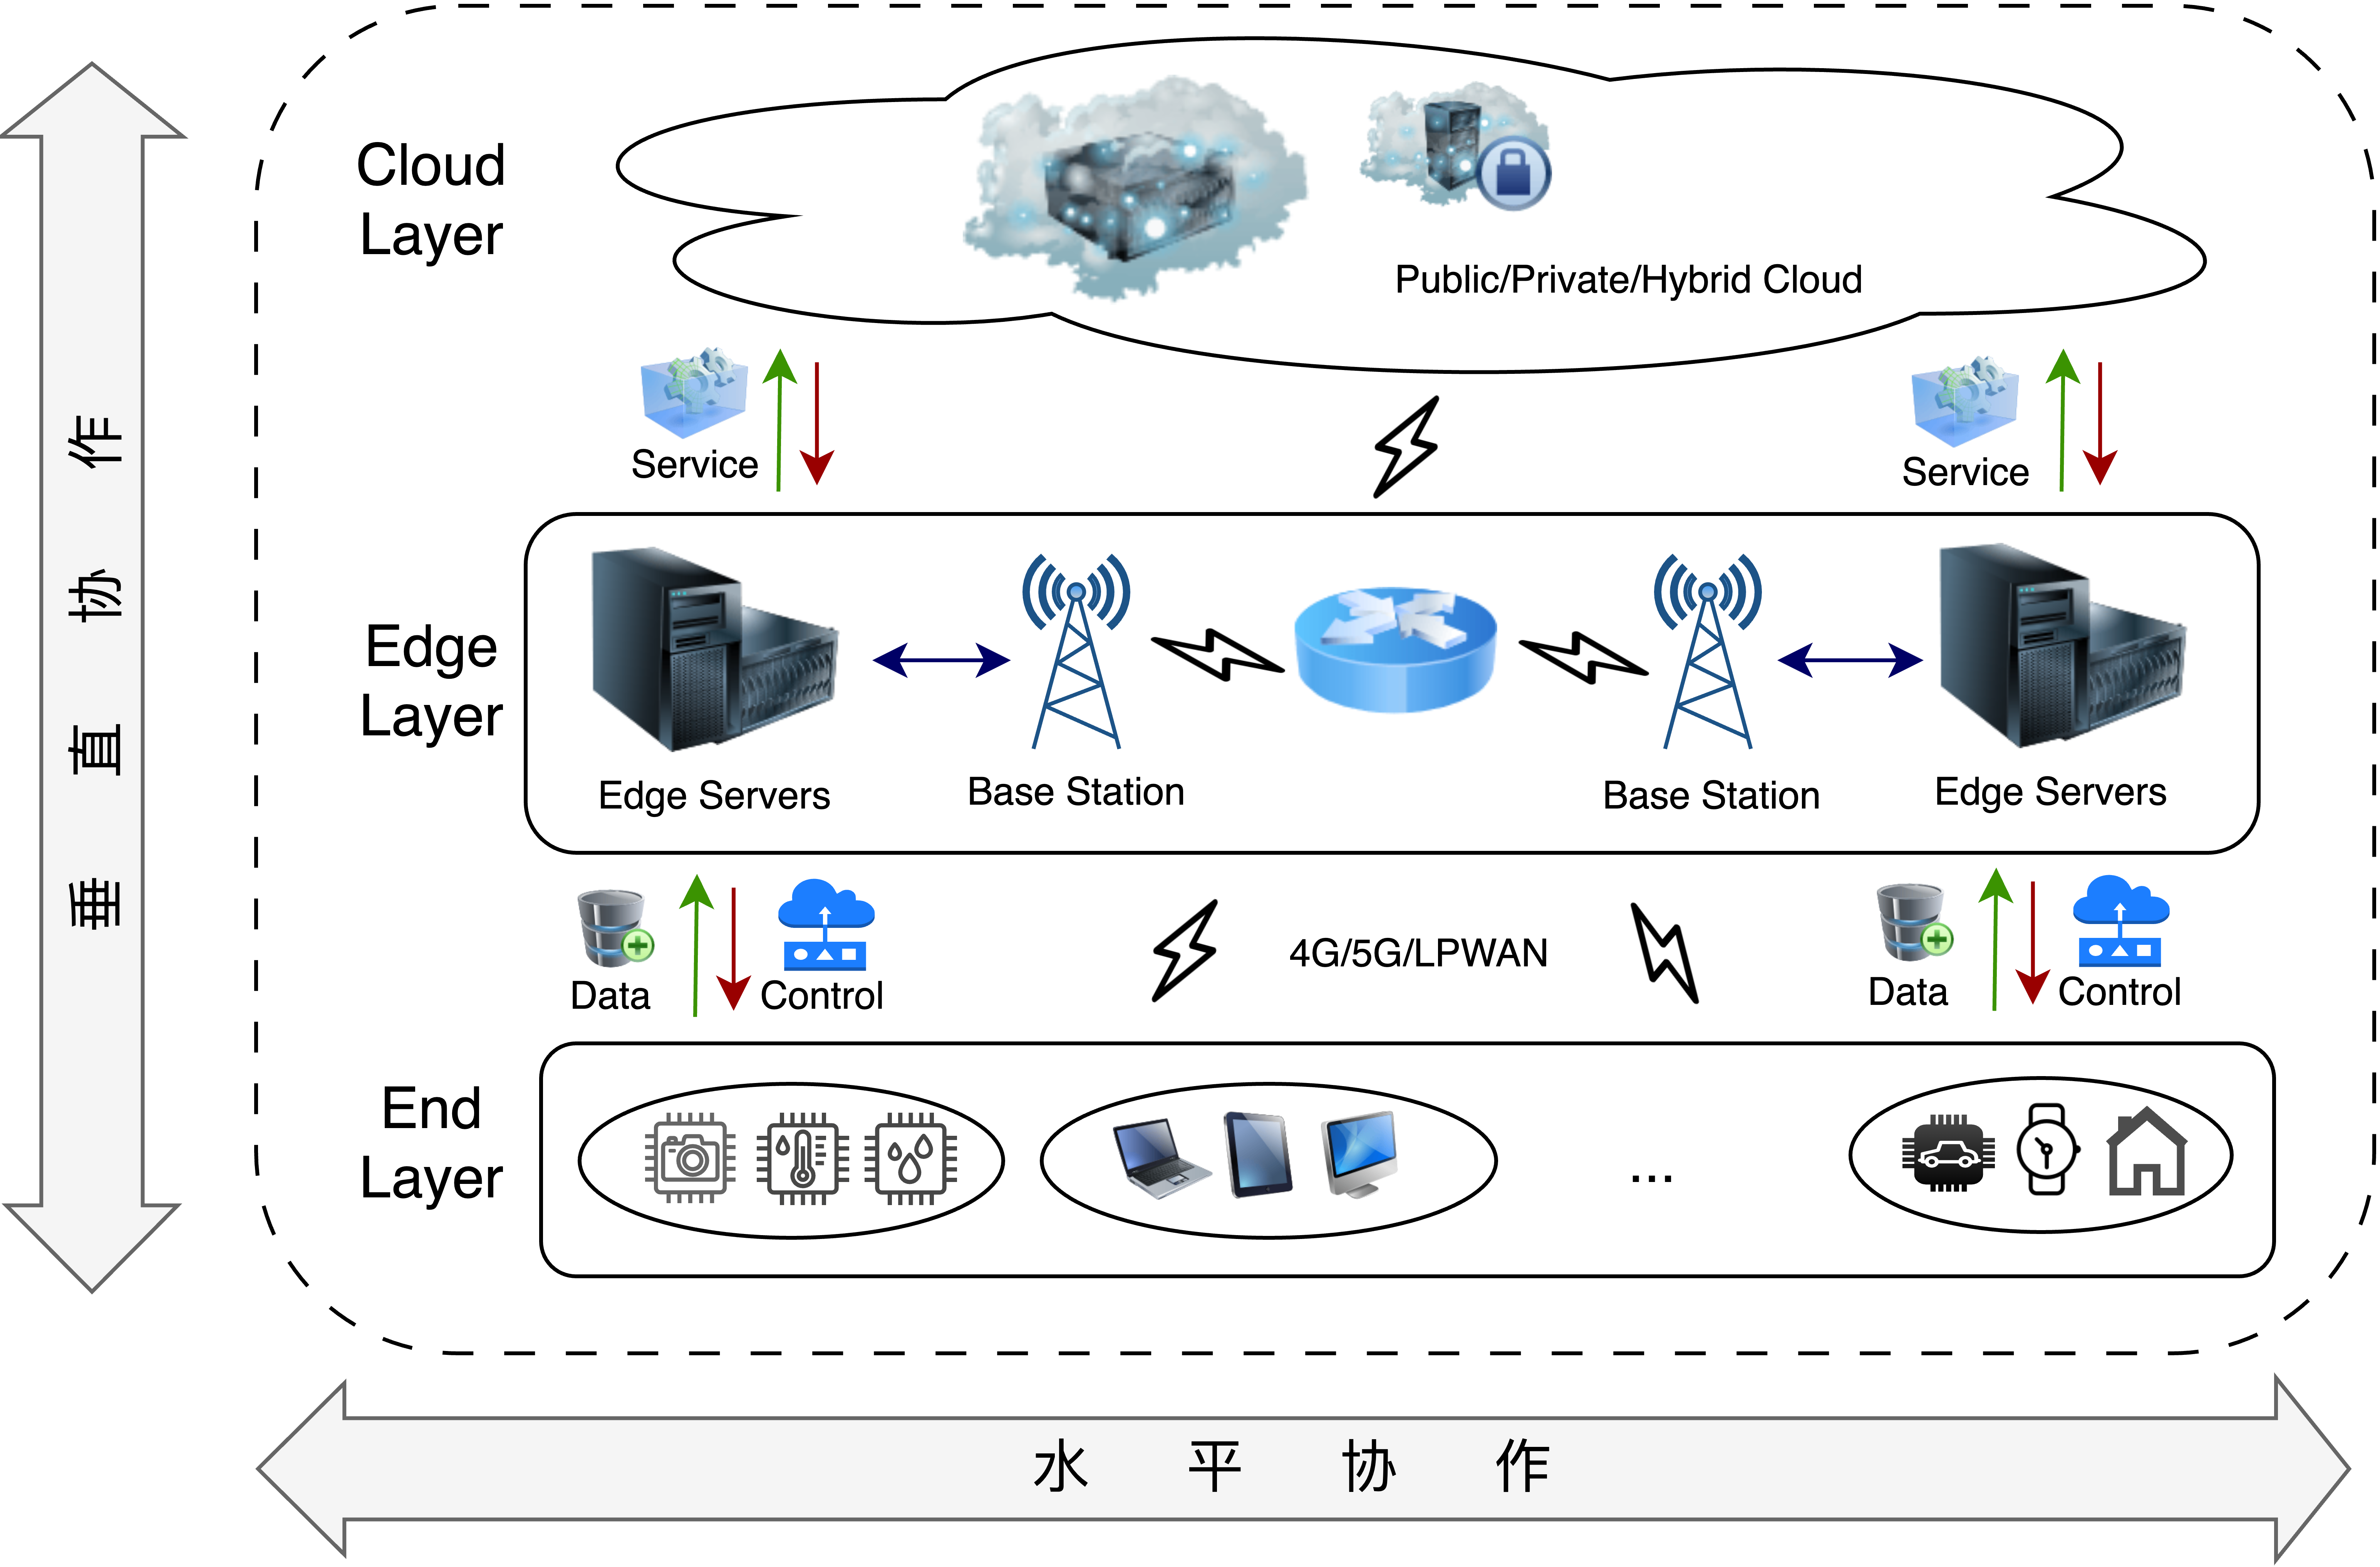
\includegraphics[width=\linewidth]{pics/2-1云边端架构.png}
  \caption{云边协同的“端-边-云”三层架构}
  \label{fig:2-1云边端架构}
\end{figure}

部分研究\cite{lane2016deepx,teerapittayanon2017distributed,liu2023adaptive}进一步指出,具有初步计算能力的端层设备也可与边缘服务器协同完成推理任务。为便于论述,本研究将这类端层设备与边层节点统一视为“边缘端”,而将云层节点称为“云端”。通过这种分层架构,云边协同能够有效利用不同层级的计算资源,从垂直和水平两个角度进行资源优化\cite{dupont2017edge,li2020elastic}。垂直优化指的是在“端-边-云”各层之间进行资源分配与优化,需要将云端和边缘端的硬件资源进行虚拟化抽象,并依据应用需求统一管理与分配。基于应用特性,计算任务可以被合理地部署在云端或边缘端,同时在层次之间需优化传输路径协议,并采取加密等手段保障数据安全。水平优化则关注同一层级内的资源协同,特别是边缘节点之间的协作计算。通过任务分割和并行计算,水平优化能够提升计算效率。通过动态监测边缘节点的负载情况,系统能够将计算任务合理分配到负载较轻的节点,进而利用负载均衡算法优化资源的使用,提升整体计算性能。

\subsection{云边协同中推理服务的供应现状}

深度学习模型通过训练实现推理功能,即通过学习大规模数据提取特征并优化参数,从而在推理阶段快速生成预测结果。模型训练因其计算和 I/O 密集性长期是研究优化的重点,而推理虽无需复杂迭代算法,通常被认为较为简单。然而,随着深度学习应用的快速发展,推理不仅需要满足更高的实时性要求,还需应对海量传感设备带来的急剧增长需求,这对系统性能和资源分配提出了严峻挑战。

目前,深度学习推理服务的供应主要有两种方式:一是通过边缘设备运行简单模型提供服务;二是依托远程云基础设施,通过“机器学习即服务”(MLaaS)平台运行复杂模型,以高吞吐量支持推理。然而,这两种方式在某些场景下存在局限性——边缘设备的模型难以满足精度需求,而云服务则无法达到严格的低延迟要求。在此背景下,云边协同计算通过结合云与边缘的优势,利用智能资源编排和优化调度机制,在性能与延迟之间实现有效权衡,在深度学习模型调度中发挥了重要作用。

尽管如此,目前大多数推理服务解决方案,如 TensorFlow Serving\cite{olston2017tensorflow} 和 Azure ML\cite{chappell2015introducing},主要面向云端推理服务的供应问题。然而,这些解决方案在应对复杂推理需求和多样化应用时存在一定局限性,尤其是在延迟和吞吐量方面。为了解决这些问题,Crankshaw 等人\cite{crankshaw2017clipper} 提出了 Clipper 系统。Clipper 通过实现预测缓存,减少了频繁查询带来的延迟和系统负载,并利用自适应批处理技术,根据模型容器的延迟配置文件动态调整批处理大小,从而优化了吞吐量与延迟之间的平衡。Clipper 还通过模型抽象层简化了不同机器学习框架之间的差异,使得开发者能够专注于模型的部署和优化,而无需关注底层框架的选择。在此基础上,Crankshaw 等人\cite{crankshaw2020inferline}提出了 InferLine,一个用于配置和管理机器学习推理管道的系统。InferLine 专注于在异构并行硬件上以低成本满足端到端延迟要求,系统通过为每个模型创建性能配置文件并估算管道的端到端延迟,优化了管道的资源分配。它还能根据实际工作负载的变化,动态调整管道配置,在负载增加时自动扩展副本数,并在负载减小时根据最小供应比率缩减副本数,从而确保系统始终满足延迟和吞吐量要求。此外,Mao 等人\cite{mao2019learning} 提出了名为 Decima 的架构,基于强化学习调度策略,可以在无需人工输入复杂调度算法的情况下,根据不同工作负载和环境条件自动学习最优策略,从而提高集群资源的利用率。然而,以上这些解决方案主要解决了云端推理服务的供应问题,并未充分考虑边缘端节点的特殊需求,尤其是在小型集群和网络延迟至关重要的地理分布式基础设施中。例如,这些方案都没有考虑不同计算节点之间的网络延迟,而在云端部署环境中,网络延迟往往可以忽略不计。

针对边缘端推理服务供应问题,目前相关研究仍然较少。一些研究提出了模型拆分技术,通过将深度学习模型的执行分布到多个离散计算单元上,以适应移动硬件平台的资源限制。Lane 等人\cite{lane2016deepx} 提出了 DeepX 框架,专注于优化深度学习模型在移动设备上的推理性能。该框架通过运行时层压缩(RLC)和深度架构分解(DAD)两种核心算法有效缓解了移动设备资源受限的难题。RLC 方法利用奇异值分解(SVD)对模型权重进行压缩,显著降低计算量和内存占用,同时通过引入估计器控制压缩程度,确保模型准确性保持在可接受范围内。DAD 方法则通过将复杂的深度模型分解为多个单元块,并将其分配到本地和远程处理器上,最大化资源利用效率。在推理过程中,这些单元块的计算结果会被重组,生成最终的预测输出。此外,Teerapittayanon 等人\cite{teerapittayanon2017distributed} 提出了分布式深度神经网络(DDNN)架构,以应对分布式计算层次结构上运行深度神经网络(DNN)时的诸多挑战。DDNN 架构通过将训练好的 DNN 映射到本地、边缘和云端的异构物理设备上,有效解决了设备资源受限和通信成本过高的问题。然而,模型拆分技术与本文研究的模型调度方法是正交的,两者各自解决不同层面的问题,为未来进一步结合两种技术提供了可能性。这种结合可以为边缘计算场景下的深度学习推理服务提供更高效、更灵活的解决方案。

\subsection{KubeEdge及相关技术}

KubeEdge 是由华为主导开发的一款轻量级开源边缘计算平台,旨在解决边缘计算场景中的关键问题,例如边缘节点与云端之间的网络管理,以及边缘节点离线时的会话维护。其架构由云端核心(Cloud Core)和边缘核心(Edge Core)两部分组成,如图 \ref{fig:2-3kubeedge} 所示。云端核心主要负责统一管理分布式的边缘应用服务,而边缘核心则运行在地理上分布的边缘节点中,为物联网应用服务提供支持。

\begin{figure}[ht]
  \centering
  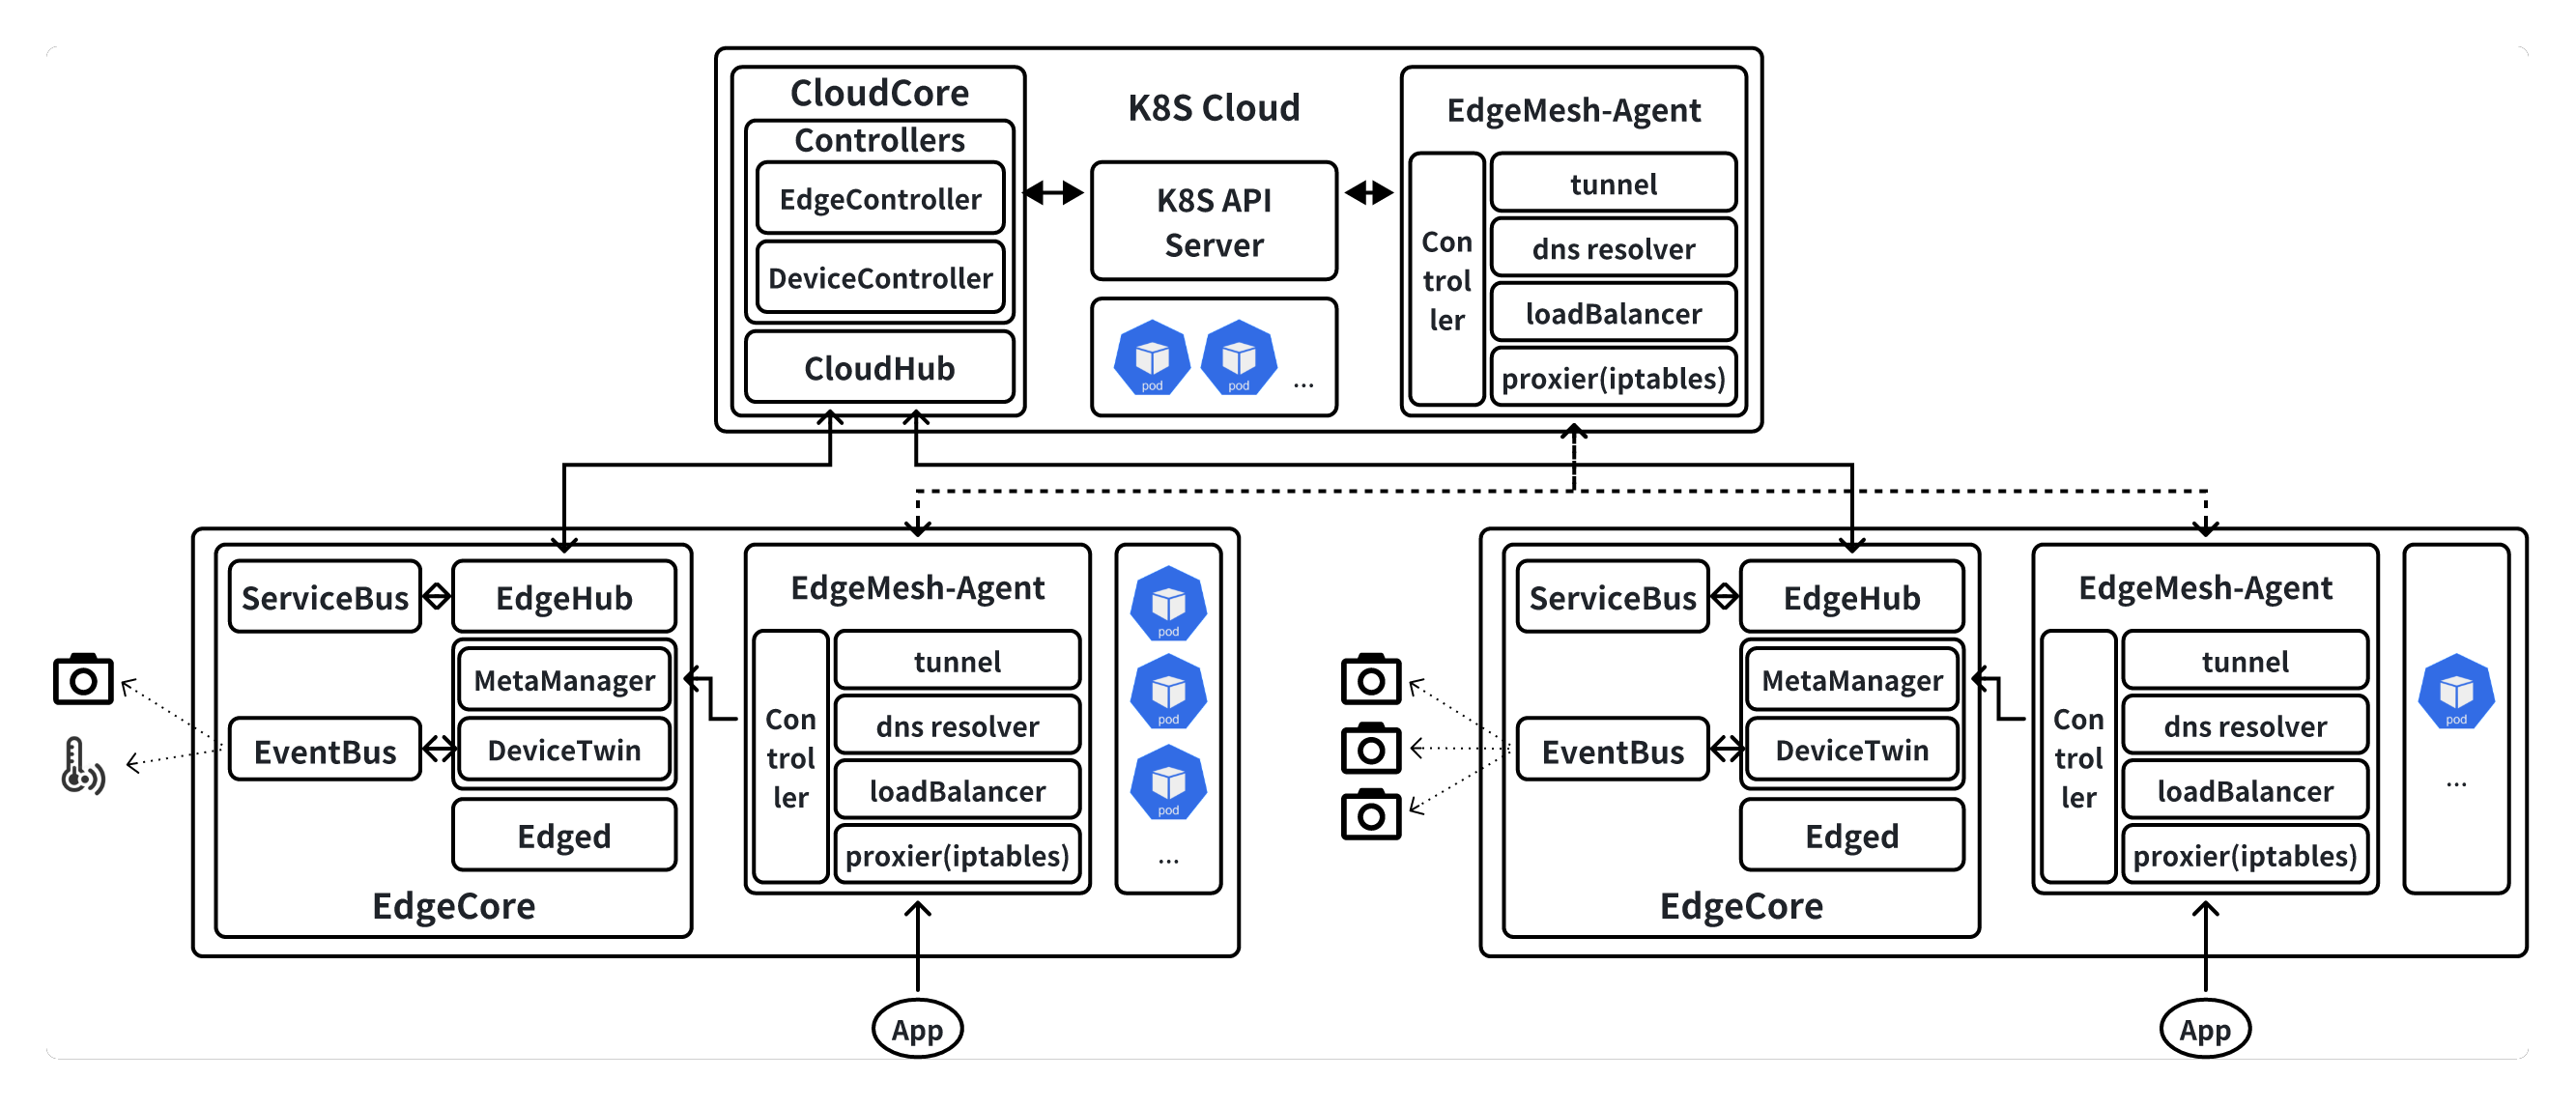
\includegraphics[width=\linewidth]{pics/2-2kubeedge.png}
  \caption{kubeedge的基础架构}
  \label{fig:2-3kubeedge}
\end{figure}

云端核心由控制器(Controller)和 CloudHub 两个组件组成,其中控制器分为边缘控制器(Edge Controller)和设备控制器(Device Controller):边缘控制器负责 Kubernetes API Server 和边缘核心之间的事件同步,而设备控制器专注于物联网设备的管理与更新;CloudHub 则作为控制器与边缘核心之间的通信中介,负责监控云端状态变化、缓存消息,并通过 socket 实现双向通信。

边缘核心主要包括以下五个组件:EdgeD 负责运行和管理基于容器的应用,支持 pod 管理、生命周期事件生成、机密管理、容器运行时支持以及工作负载部署;EdgeHub 负责边缘与云端之间的通信,通过 socket 连接实现资源同步、设备状态更新及消息转发;EventBus 提供 MQTT 客户端交互功能,支持发布/订阅机制;DeviceTwin 用于存储设备状态并同步到云端,同时为应用提供查询接口;MetaManager 作为 EdgeD 和 EdgeHub 之间的消息处理器,负责元数据的存储与检索。

EdgeMesh 是 KubeEdge 集群的数据平面组件,主要提供高可用支持、服务发现和流量代理功能。它利用 LibP2P 技术在边缘节点之间搭建通信网络:对于局域网内的节点,直接访问即可完成数据交互;在跨局域网场景下,则通过打洞隧道技术或中继流量实现数据传输。此外,EdgeMesh 借助 EdgeHub - CloudHub 隧道分发元数据,从而无需直接访问云端,并通过在节点层面部署的 DNS 服务器提升服务搜索的可靠性。在负载均衡方面,EdgeMesh 采用 Istio 的目标规则(DestinationRule),提供轮询和随机等方案,以确保流量在各 Pod 间高效分配,如图 \ref{fig:2-3edgemesh} 所示。

\begin{figure}[ht]
  \centering
  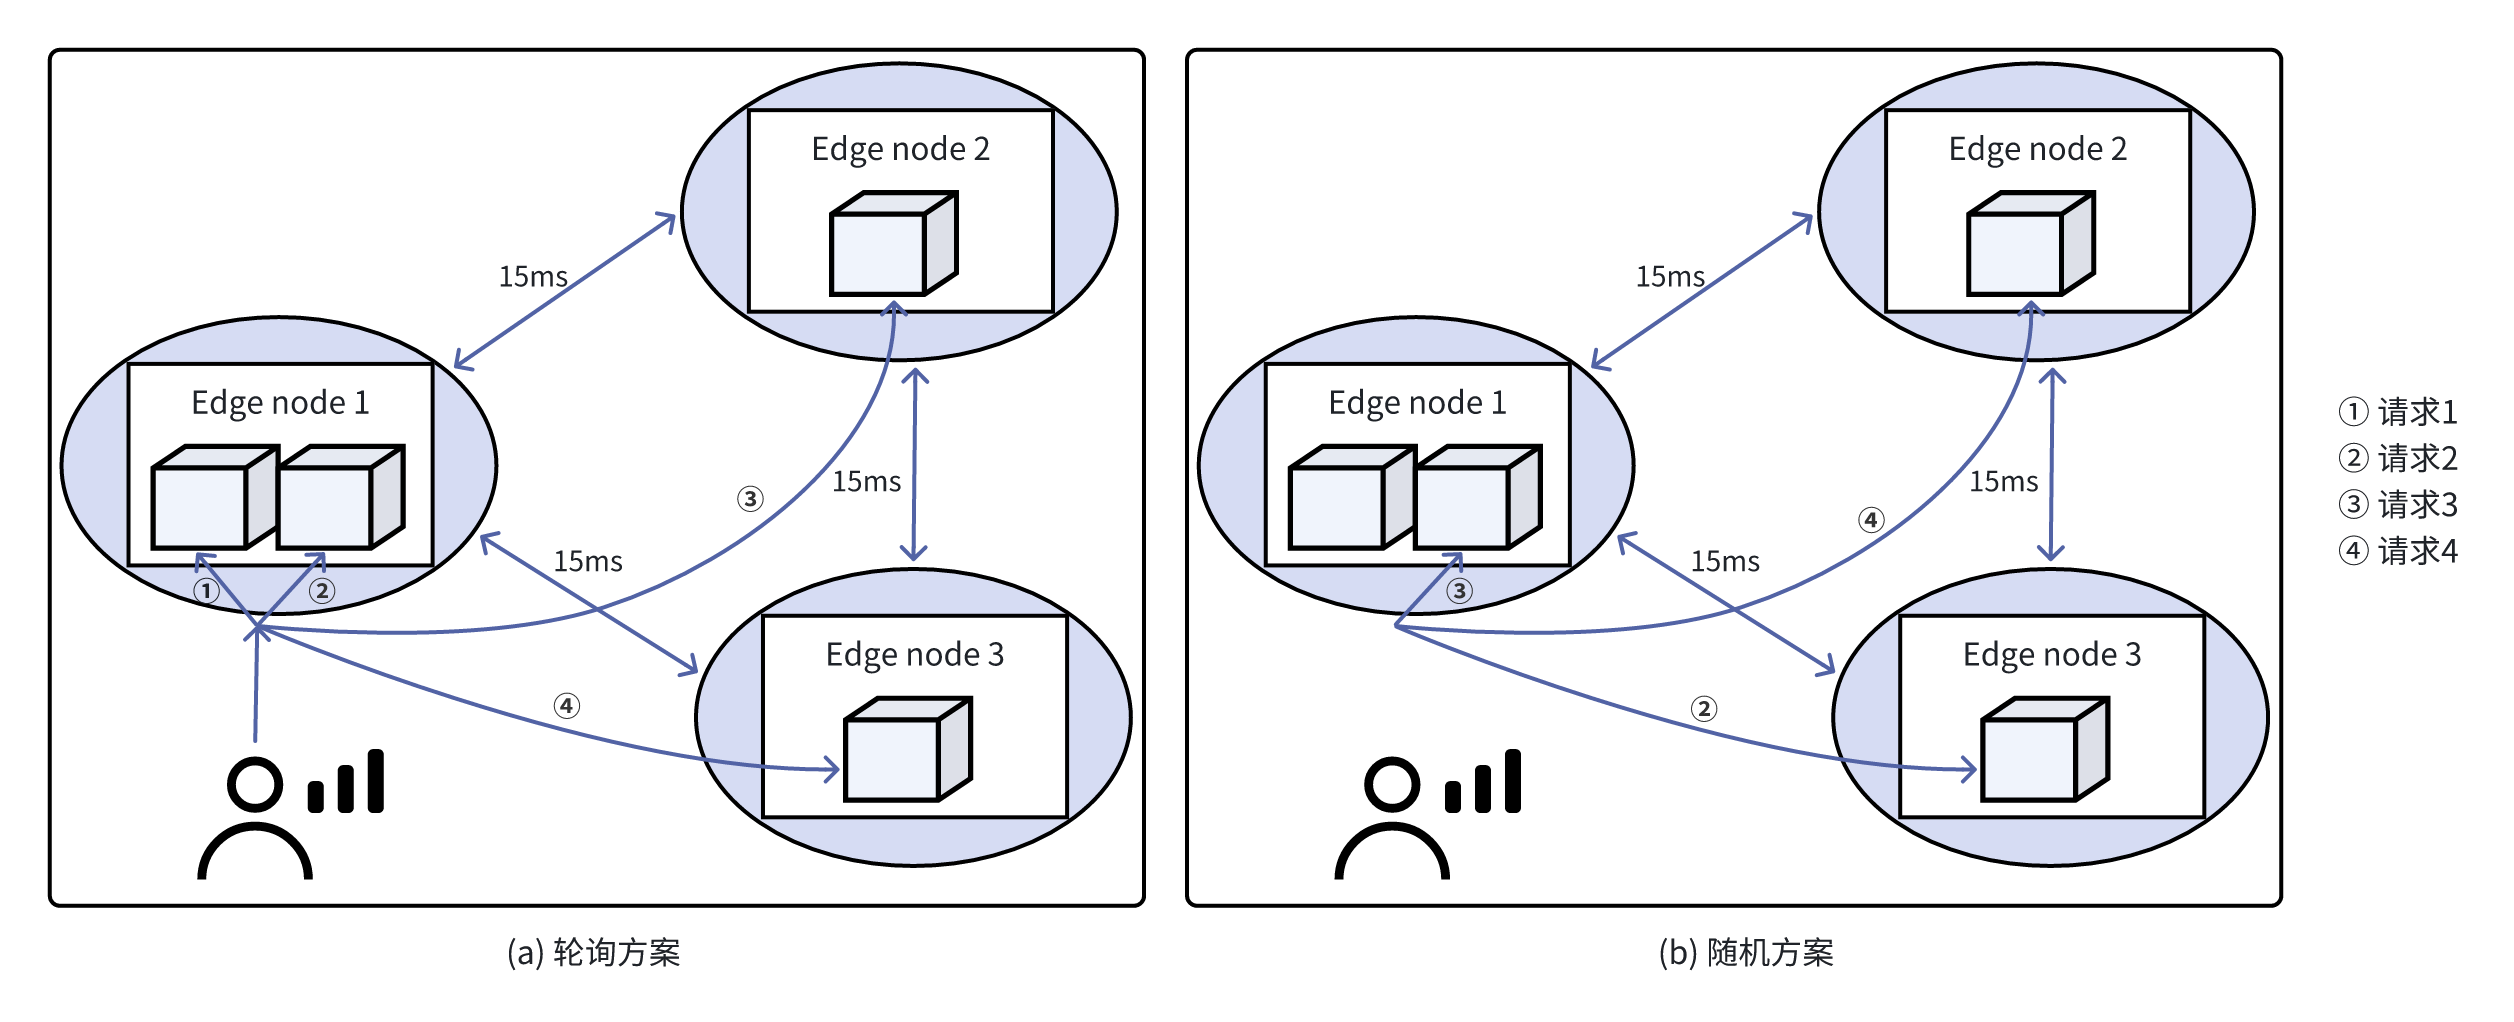
\includegraphics[width=\linewidth]{pics/2-3edgemesh.png}
  \caption{KubeEdge 中的负载均衡方案}
  \label{fig:2-3edgemesh}
\end{figure}

然而,EdgeMesh 并未考虑边缘节点间转发请求所带来的额外延迟。由于边缘计算环境中节点通常地理位置分散,跨节点间的流量转发会显著增加网络时延,降低集群整体吞吐量。针对此问题,Kim 等人\cite{kim2023local}提出了本地调度方案:当边缘节点收到用户请求后,将其平均分配给同一节点上的 Pod,而非转发给远程节点。这样不仅避免了跨节点流量转发导致的高延迟,还能在本地边缘节点即时处理用户请求,从而提升系统的整体吞吐量。然而,本地调度方案也存在不足之处。由于边缘端基础设施通常故障率较高且维护成本较高,当某节点掉线时,部分请求可能无法满足服务质量需求。为解决这些问题,Haja 等人\cite{haja2019sharpening} 提出了 Pod 占位符机制。该机制通过调度算法为每个 Pod 分配一个具有反亲和性(Anti-Affinity)的占位符。当 Pod 所在的主机节点发生故障时,占位符可以迅速在符合延迟约束的其他节点上重新启动 Pod,从而确保服务的连续性。但是,该方法主要关注单节点的可靠性,未能充分利用分布式边缘节点之间的协同能力,限制了系统在高负载场景下的扩展性和整体可靠性。

KubeEdge 的负载 Pod 调度过程依赖于云端 Kubernetes 的调度机制,如图 \ref{fig:2-4k8sschedule} 所示。云端的 Kubernetes 调度器(kube-scheduler)通过监听未分配节点的 Pod,采用两步法选择最佳节点:首先,通过过滤(Filtering)策略(如资源需求、亲和性、反亲和性等),排除不符合条件的节点,生成可行节点列表;接着,通过打分(Scoring)策略(如资源平衡、数据本地性等),对可行节点进行评分,并选择得分最高的节点。如果存在多个得分相同的节点,则随机选择一个进行绑定。

\begin{figure}[ht]
  \centering
  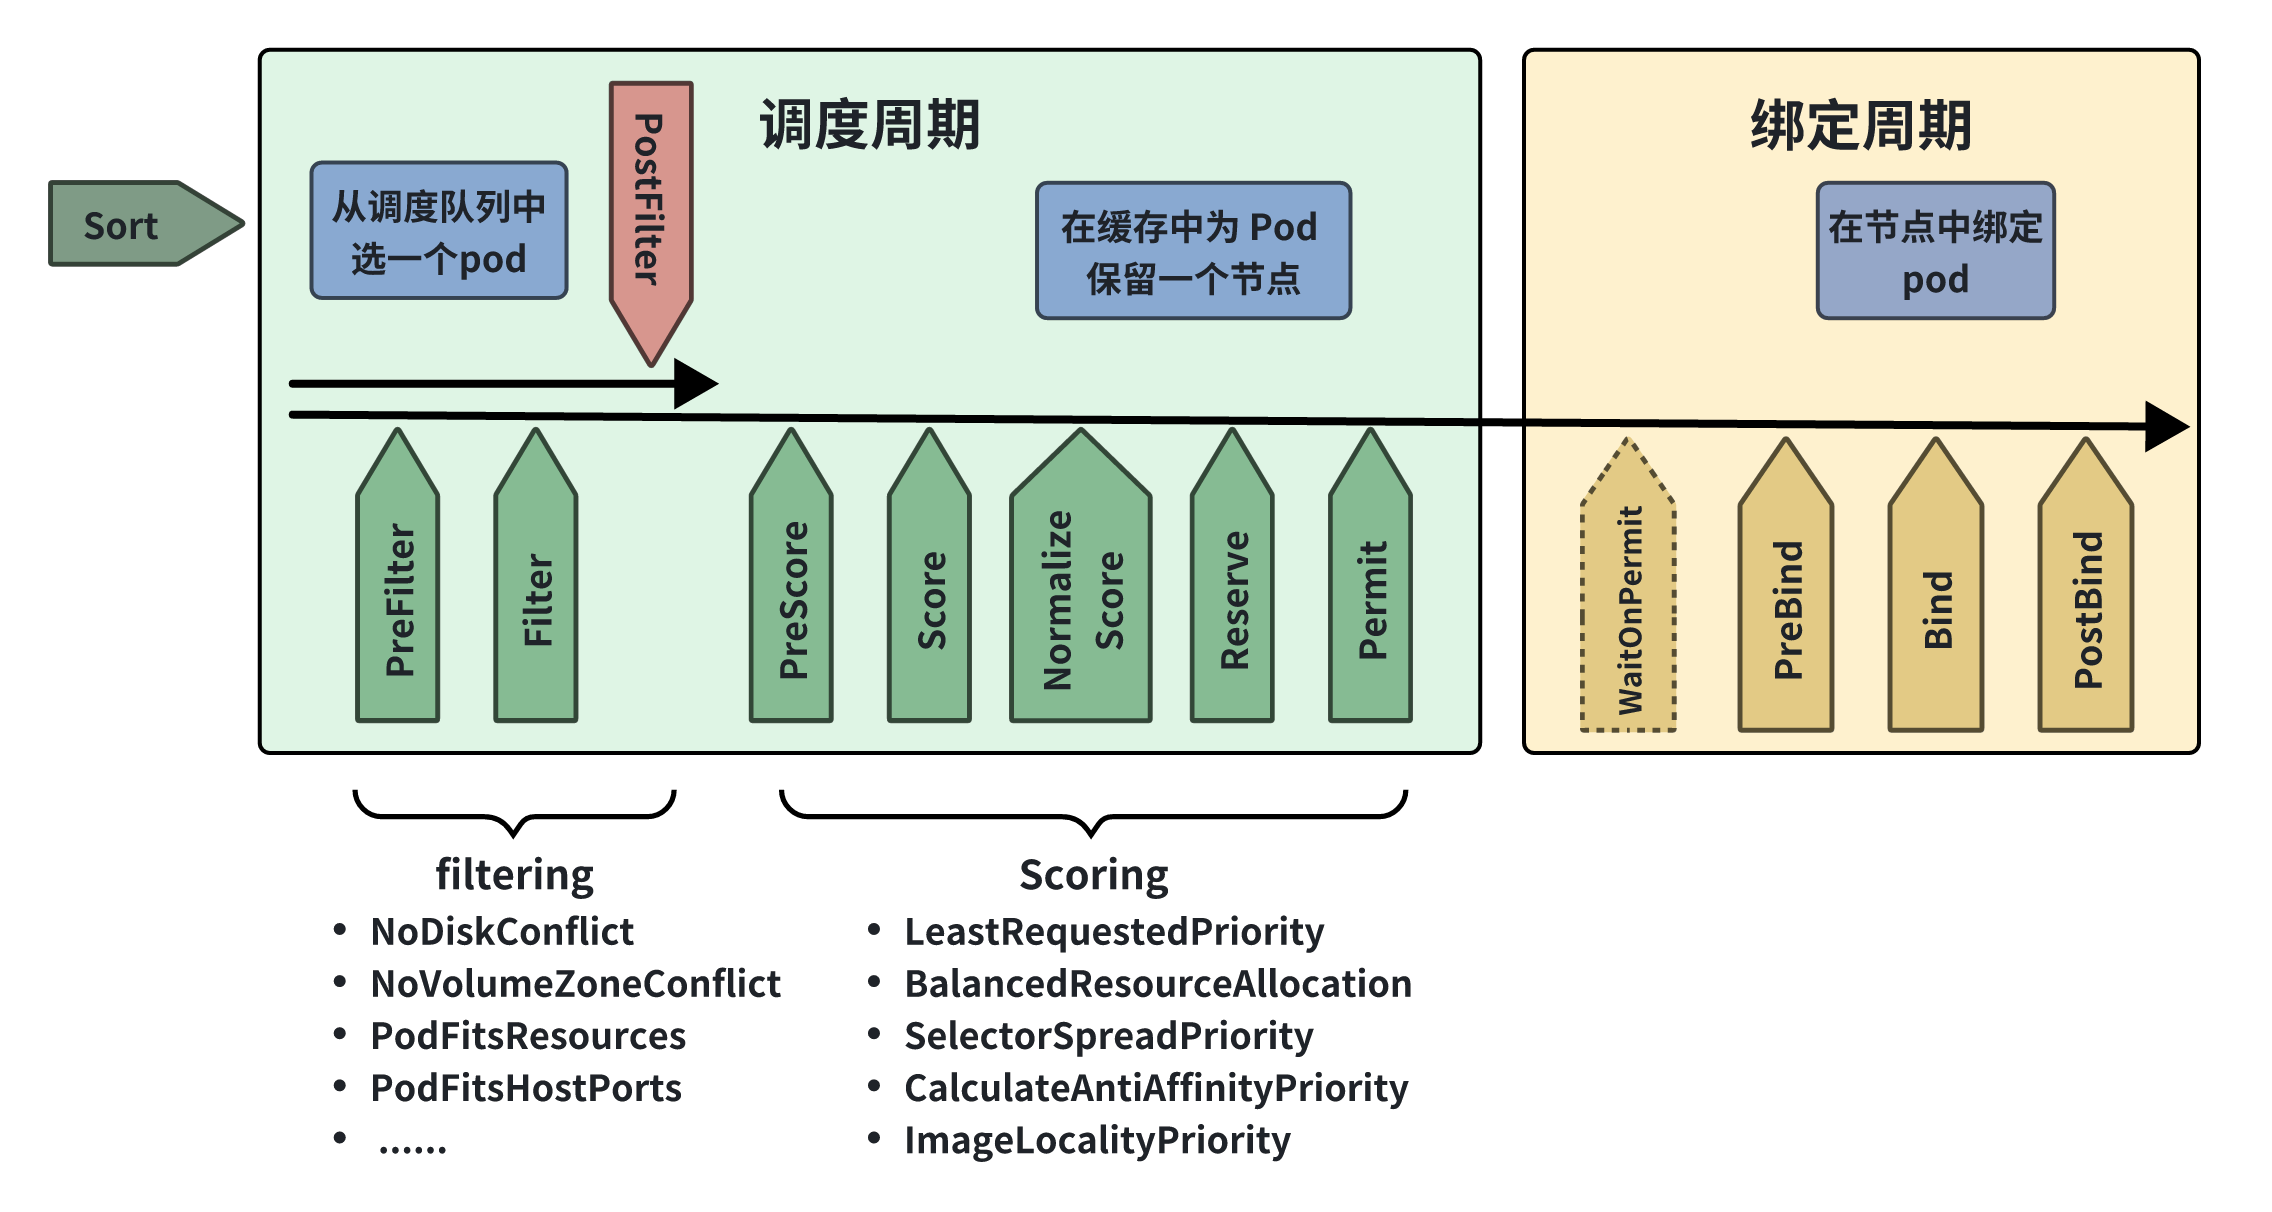
\includegraphics[width=\linewidth]{pics/2-4k8sschedule.png}
  \caption{Kubernetes 中的负载调度方案}
  \label{fig:2-4k8sschedule}
\end{figure}

然而,Kubernetes 的调度逻辑主要针对云端高性能节点设计,在边缘环境中存在适配性不足的问题,面临资源协调与应用协作管理的双重挑战。在资源协调方面,云边网络具有松散耦合的结构和较高的通信时延,导致云端调度器难以及时掌握边缘资源的实时利用率,从而无法在最佳时机完成任务的优化调度。在应用协作方面,现有云端调度机制对用户服务质量的感知和支持不足,难以有效应对云边协同应用中任务的垂直卸载和水平迁移需求,这进一步增加了应用协作管理的复杂性。

为了解决上述问题,Lingayya 等人\cite{lingayya2024dynamic} 提出了一种创新的资源管理与任务调度方案,旨在提高边缘计算环境的适应性和运行效率。该方案在边缘节点部署高效的监测模块,实时采集设备资源状态(包括计算能力、内存使用、网络带宽等)和任务队列信息,同时利用多智能体协同强化学习方法,通过多个智能体在共享环境中协作,综合各自的目标和能力,优化整体系统性能。此外,Shan 等人\cite{shan2024kces} 提出了一种资源分配算法。当资源评估结果显示当前节点无法满足任务需求时,该算法通过动态调整任务的资源分配方案,使节点能够容纳更多任务,同时确保任务的最小资源需求,从而最大化资源利用率。如果调整后资源仍无法满足需求,则通过任务水平迁移,将任务分配到其他边缘节点。此外,该方案结合设备的监控模式,对任务进行合理卸载,选择合适的边缘节点或云节点执行,从而实现云边协同的垂直卸载。然而,上述方案主要面向通用负载,对深度学习模型的适配能力较低,难以以低成本高效地获取负载的运行时延,仍存在一定的改进空间。

\section{边缘端节点监测技术}

边缘端通常由多种类型的节点组成,包括硬件配置各异的设备和具有不同网络带宽与延迟特性的连接\cite{cooke2020model,varghese2021survey,barbalace2020edge}。例如,这些节点可能配备低功耗的 CPU、高并行处理能力的多核 GPU,或专用的 AI 加速器(如 VPU)等硬件资源。这种硬件和网络特性的异构性导致节点在计算能力、存储容量和能耗限制上存在显著差异,从而显著增加了资源分配与利用优化的复杂性。

\subsection{边缘端节点推理能力监测技术}

对于深度学习推理来说,模型的计算需求必须适配目标设备的硬件特性,但异构环境下的适配和模型迁移需要对任务进行细粒度划分和动态调整,从而大幅增加了调度的复杂性。在边缘端,评估深度学习推理性能的关键指标是推理时延。传统的基于测量的方法需要复杂的部署过程,尤其在多样化的边缘设备和推理框架场景下,难以应对设备数量的快速增长。现有的基于FLOPs的方法在预测准确性上存在不足,无法满足实际需求。

为了解决这一问题,Zhang 等人\cite{zhang2021nn} 提出了 nn-Meter 工具,如图 \ref{fig:2-5nnmeter} 所示。该工具通过设计测试用例,自动检测模型在不同边缘设备上的推理执行单元(内核),并基于检测到的融合规则,递归地将模型划分为内核,从而有效捕获不同设备上的算子融合行为,大幅提高了预测的准确性。nn-Meter 的核心技术包括以下几个方面:首先,根据模型设计和硬件延迟特性对内核配置进行剪枝;其次,通过迭代采样过程自动选择最优配置进行检测,而非采用随机选择策略;最后,利用机器学习回归器学习采样数据的非线性关系,构建高效的内核级延迟预测器。这一方法显著降低了数据采样成本,同时大幅提高了预测准确性。在 nn-Meter 工具的基础上,本文进一步对其进行了改进,使其适配云原生环境,能够在不同资源隔离策略下进行推理时延预测。通过这些改进,系统不仅能够满足多样化边缘设备的性能评估需求,还能够更好地支持云边协同环境下的推理任务优化。

\begin{figure}[ht]
  \centering
  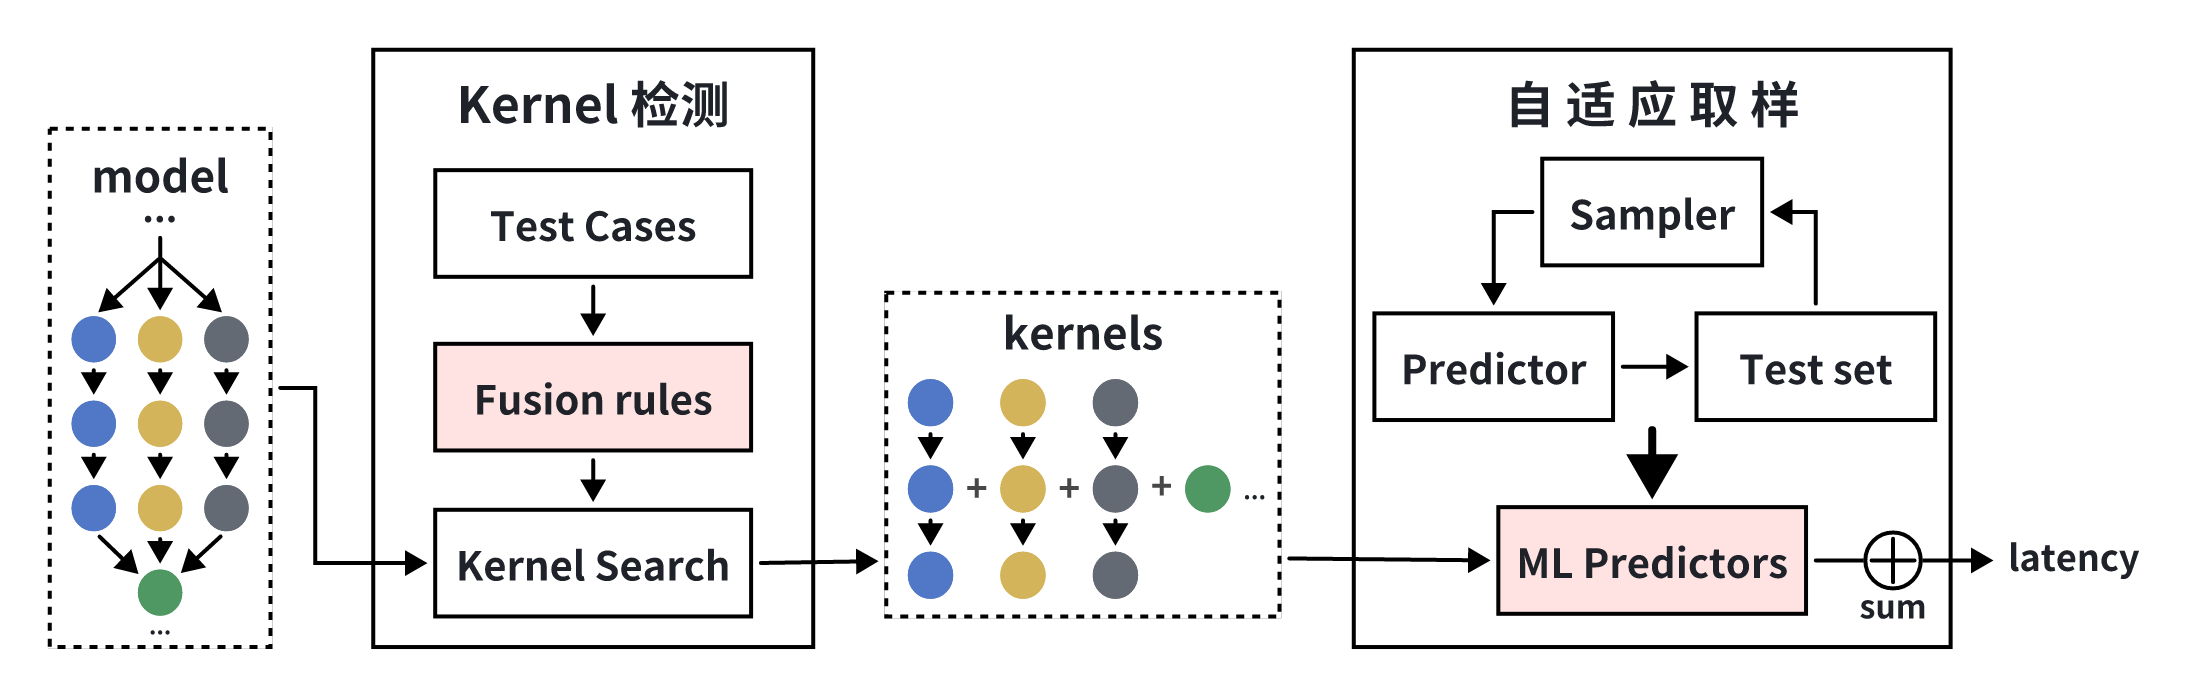
\includegraphics[width=\linewidth]{pics/2-5nnmeter.png}
  \caption{nn-Meter工具的架构}
  \label{fig:2-5nnmeter}
\end{figure}

\subsection{边缘端节点间通信监测技术}

边缘端节点通常分布在异构网络环境中,其通信性能容易受到网络带宽、延迟、丢包率以及通信协议开销等多种因素的影响。为了解决这一问题,Haja 等人\cite{haja2019sharpening} 提出了一种实时监测边缘节点间传输时延的方法。该方法在每个节点上部署测量 Pod,这些 Pod 定期发送 ping 包并记录往返时间,从而生成延迟数据,如图 \ref{fig:2-6ping} 所示。此设计能够提供实时的通信性能评估,为动态优化和调度策略的制定提供数据支持。

\begin{figure}[ht]
  \centering
  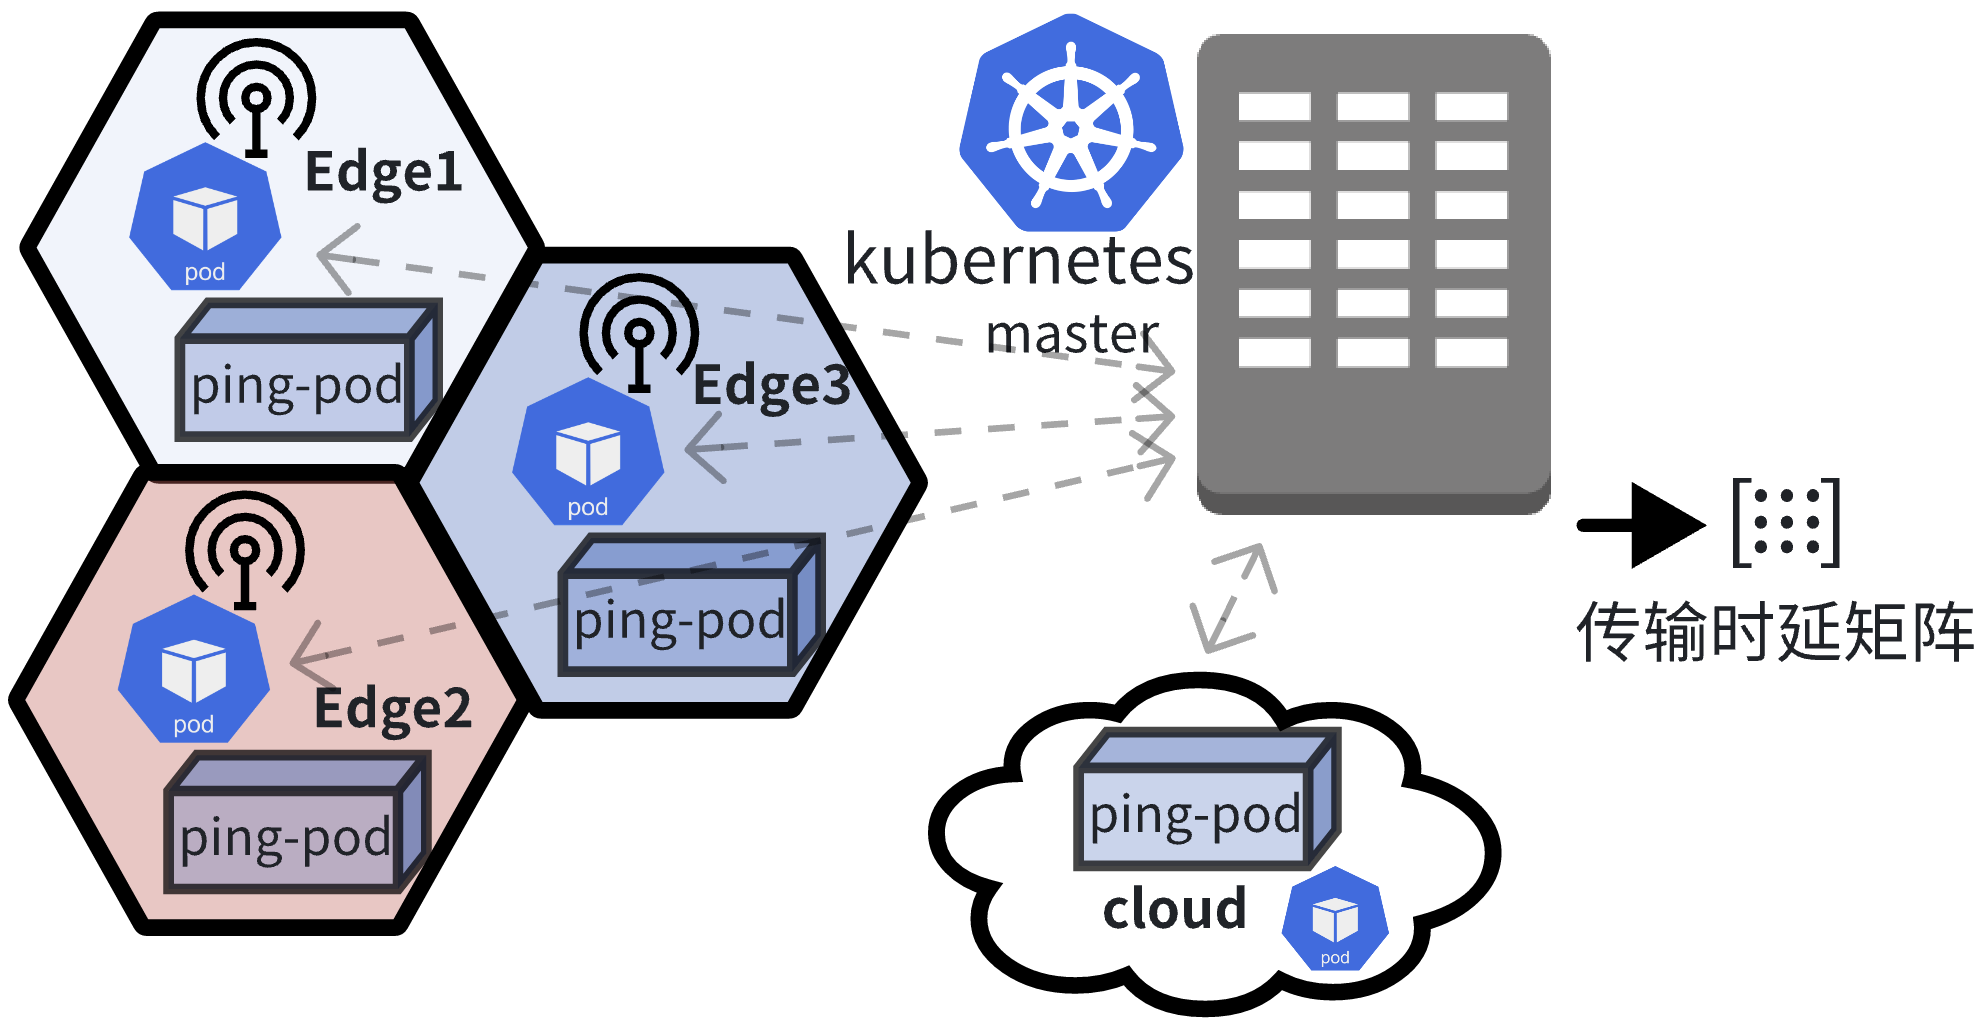
\includegraphics[width=0.7\linewidth]{pics/2-6ping.png}
  \caption{测量并记录传输时延矩阵的过程}
  \label{fig:2-6ping}
\end{figure}

在边缘节点间通信监测中,Ping、iperf3 和 Prometheus + Blackbox Exporter 是三种常用的技术方案,各有其特点和适用场景。Ping 是一种轻量级工具,通过发送 ICMP 请求快速检测网络连通性和往返延迟(RTT),适用于实时性要求高的基础连通性监测,但其功能较为单一,无法提供带宽等深入的性能数据。相比之下,iperf3 提供更详尽的网络性能指标,包括带宽、抖动和丢包率,支持 TCP 和 UDP 协议,适合需要深入分析网络质量的场景。然而,iperf3 的部署较为复杂,且因其占用较多网络资源,不适合实时或生产环境的持续监测。Prometheus + Blackbox Exporter 专注于大规模分布式系统的长期监控,通过周期性探测提供延迟和可用性等性能数据,同时支持多种协议的探测和丰富的数据分析功能,但其配置复杂且在实时性要求较高的场景中可能存在一定延迟。

\section{本章小结}

本章首先系统性地阐述了云边协同的基本概念及其分层架构,并聚焦于云边协同中深度学习推理服务的供应问题,回顾了现有的云端和边缘端推理服务解决方案。随后,详细介绍了本文原型系统所依托的 KubeEdge 架构及其主要服务功能。最后,针对边缘端节点的异构性和复杂性,系统梳理了推理能力监测与通信性能监测技术的最新进展。通过对以上内容的总结,本章不仅为后续研究提供了必要的背景知识和技术支撑,还明确了云边协同在深度学习推理服务中的关键挑战及其潜在解决路径。




\chapter{云边协同下深度学习推理服务的调度方法}

\section{推理服务网络模型}

\subsection{模型定义}

\subsection*{1. 节点定义}

\subsubsection*{1.1 云端节点}
设云端节点集合为 \( C = \{c_1, c_2, \dots, c_m\} \)。每个云端节点 \( c_i \) 定义如下:
\begin{itemize}
    \item \(\text{CPU}(c_i)\):云端节点 \( c_i \) 的 CPU 容量。
    \item \(\text{MEM}(c_i)\):云端节点 \( c_i \) 的内存容量。
    \item \(\text{GPU}(c_i)\):云端节点 \( c_i \) 的 GPU 容量。
    \item \(\text{BW}(c_i)\):云端节点 \( c_i \) 的带宽容量(单位:数据大小/时间)。
\end{itemize}

\subsubsection*{1.2 边端节点}
设边端节点集合为 \( E = \{e_1, e_2, \dots, e_n\} \)。每个边端节点 \( e_j \) 定义如下:
\begin{itemize}
    \item \(\text{CPU}(e_j)\):边端节点 \( e_j \) 的 CPU 容量。
    \item \(\text{MEM}(e_j)\):边端节点 \( e_j \) 的内存容量。
    \item \(\text{BW}(e_j)\):边端节点 \( e_j \) 的带宽容量。
    \item \(\text{GPU}(e_j) = 0\):边端节点没有 GPU 资源。
\end{itemize}

\subsection*{2. 用户请求定义}
设用户请求集合为 \( R = \{r_1, r_2, \dots, r_k\} \)。每个用户请求 \( r_i \) 定义如下:
\begin{itemize}
    \item \(\text{ID}(r_i)\):请求的唯一标识符。
    \item \(\text{Type}(r_i)\):请求的类型,表示需要处理的 AI 任务类型。
    \item \(\text{Duration}(r_i)\):请求的运行周期时长(单位:时间)。
    \item \(\text{DataCount}(r_i)\):请求包含的数据数量。
    \item \(\text{DataSize}(r_i)\):请求的数据总大小(单位:数据大小)。
    \item \(\text{Accuracy}(r_i)\):请求要求的最低准确率。
    \item \(\text{Source}(r_i)\):请求的节点来源(可以是某个边端节点 \( e_j \))。
\end{itemize}

\subsection*{3. AI 负载定义}
设 AI 负载集合为 \( A = \{a_1, a_2, \dots, a_p\} \)。每个 AI 负载 \( a_i \) 定义如下:
\begin{itemize}
    \item \(\text{ID}(a_i)\):AI 负载的唯一标识符。
    \item \(\text{Name}(a_i)\):AI 负载的名称。
    \item \(\text{SupportedTypes}(a_i)\):能够响应的请求类型集合。
    \item \(\text{Latency\_GPU}(a_i, y)\):在 GPU 环境下,节点 \( y \) 上运行该负载的单次推理时延(单位:时间)。
    \item \(\text{Latency\_NoGPU}(a_i, y)\):在非 GPU 环境下,节点 \( y \) 上运行该负载的单次推理时延(单位:时间)。
    \item \(\text{Throughput}(a_i)\):单次推理的吞吐量(每次推理能处理的图片数量)。
    \item \(\text{Resources}(a_i) = (\text{CPU}(a_i), \text{MEM}(a_i), \text{GPU}(a_i))\):运行所需的资源量。
\end{itemize}

\subsection*{4. 调度目标与约束}

\subsubsection*{4.1 调度决策变量}
定义调度变量:
\begin{itemize}
    \item \( x_{ij} \geq 0 \):表示请求 \( r_i \) 中由 AI 负载 \( a_j \) 处理的数据比例(\(0 \leq x_{ij} \leq 1\),所有负载的比例之和为 1)。
    \item \( y_{ij} \in C \cup E \):表示请求 \( r_i \) 中分配给 AI 负载 \( a_j \) 的任务被分配到的节点(云端节点或边端节点)。
\end{itemize}

约束:
\begin{itemize}
    \item 数据分配总量约束:请求 \( r_i \) 中,分配给所有 AI 负载的数据比例之和等于 1,即:
    \[
    \sum_{j} x_{ij} = 1, \quad \forall r_i \in R
    \]
    其中,\( x_{ij} \) 表示负载 \( a_j \) 处理的比例。
\end{itemize}

\subsubsection*{4.2 约束条件}

\paragraph*{1. 运行时长约束}


\paragraph*{1. 运行时长约束}

请求 \( r_i \) 在运行周期内必须完成其所有数据的处理,约束如下:

\[
\sum_{j} \left( \frac{x_{ij} \cdot \text{DataCount}(r_i)}{\text{Throughput}(a_j)} \cdot \text{Latency}(a_j, y_{ij}) \right) + \frac{\text{DataSize}(r_i)}{\text{BW}(y_{ij})} \leq \text{Duration}(r_i), \quad \forall r_i \in R
\]

其中:
\begin{itemize}
    \item \( x_{ij} \cdot \text{DataCount}(r_i) \):表示负载 \( a_j \) 处理的具体数据量。
    \item \( \text{Throughput}(a_j) \):AI 负载 \( a_j \) 的单次推理吞吐量。
    \item \( \text{Latency}(a_j, y_{ij}) \):AI 负载 \( a_j \) 在节点 \( y_{ij} \) 上的单次推理时延。
    \item \( \frac{\text{DataSize}(r_i)}{\text{BW}(y_{ij})} \):数据传输时延,取决于请求的数据大小和节点 \( y_{ij} \) 的带宽。
    \item \( \text{Duration}(r_i) \):请求的运行周期时长。
    \item \[
            \text{Latency}(a_j, y_i) =
            \begin{cases} 
            \text{Latency\_GPU}(a_j), & \text{if } \text{GPU}(y_i) > 0 \\
            \text{Latency\_NoGPU}(a_j), & \text{if } \text{GPU}(y_i) = 0
            \end{cases}
        \]
\end{itemize}

该约束确保所有分配给负载的任务在请求时长内能够完成。

\paragraph*{2. 准确率约束}

请求的处理结果需满足其准确率要求,考虑数据分配比例后,约束如下:
\[
\sum_{j} x_{ij} \cdot \text{Accuracy}(a_j) \geq \text{Accuracy}(r_i), \quad \forall r_i \in R
\]
其中:
\begin{itemize}
    \item \( x_{ij} \cdot \text{Accuracy}(a_j) \):表示负载 \( a_j \) 处理的比例对应的贡献准确率。
    \item \(\text{Accuracy}(r_i)\):请求 \( r_i \) 对整体任务的最低准确率要求。
\end{itemize}

\paragraph*{3. 资源容量约束}
每个节点的资源总使用量不能超过其可用容量:
\[
\sum_{r_i \in R} x_{ij} \times \text{Resources}(a_j) \leq \text{AvailableResources}(y_i), \quad \forall y_i \in C \cup E
\]

\subsubsection*{4.3 优化目标}

优化目标分为两级优先级:

\paragraph*{1. 一级优化目标:最大化成功响应的请求数量}

目标是优先最大化成功响应的请求数量。定义一个二进制变量:
\[
z_i = 
\begin{cases} 
1, & \text{如果请求 } r_i \text{ 被成功响应(满足所有约束)} \\
0, & \text{否则}
\end{cases}
\]
一级优化目标为:
\[
\max \sum_{r_i \in R} z_i
\]

\paragraph*{2. 二级优化目标:在满足一级目标的基础上最小化带宽利用}

在一级目标下,进一步最小化所有请求的数据传输所消耗的带宽:
\[
\min \sum_{r_i \in R} \sum_{j} \frac{x_{ij} \cdot \text{DataSize}(r_i)}{\text{BW}(y_{ij})}
\]
其中:
\begin{itemize}
    \item \( x_{ij} \cdot \text{DataSize}(r_i) \):表示负载 \( a_j \) 处理的任务对应的数据大小。
    \item \( \text{BW}(y_{ij}) \):节点 \( y_{ij} \) 的带宽。
\end{itemize}





\subsection{推理服务调度问题的形式化表述}

\section{云边协同下的推理服务调度方法}




主动探测与被动采集结合的方法

\chapter{面向模型推理的云边协同调度系统}

本章将对面向模型推理的云边协同调度系统进行介绍。首先介绍了系统的运行平台KubeEdge的相关细节,接着介绍系统架构设计以及各个组件的设计。

\section{KubeEdge及相关技术介绍}

本文提出的面向模型推理的云边协同调度具有普适性,能够适配各类云边云原生平台。为验证其有效性,需选择具有典型代表性的云边协同平台进行落地和验证。KubeEdge作为首个获得CNCF基金会认证的边缘计算框架,其架构设计深度契合云边协同的分布式计算模式,且由华为主导的活跃开源社区持续提供技术演进保障。因此,本文选择基于KubeEdge构建KEAS系统。

\subsection{KubeEdge架构设计}

KubeEdge是一种面向云边协同场景的边缘计算框架,旨在将Kubernetes的能力从云端延伸至边缘,从而实现统一的资源管理和应用部署。如图 \ref{fig:4-1kubeedge} 所示,KubeEdge通过云端和边缘组件的紧密协作,构建了一个高效且可靠的分布式架构。该架构不仅支持边缘节点的自治运行,还能在网络条件受限的情况下保持与云端的稳定通信。

\begin{figure}[ht]
  \centering
  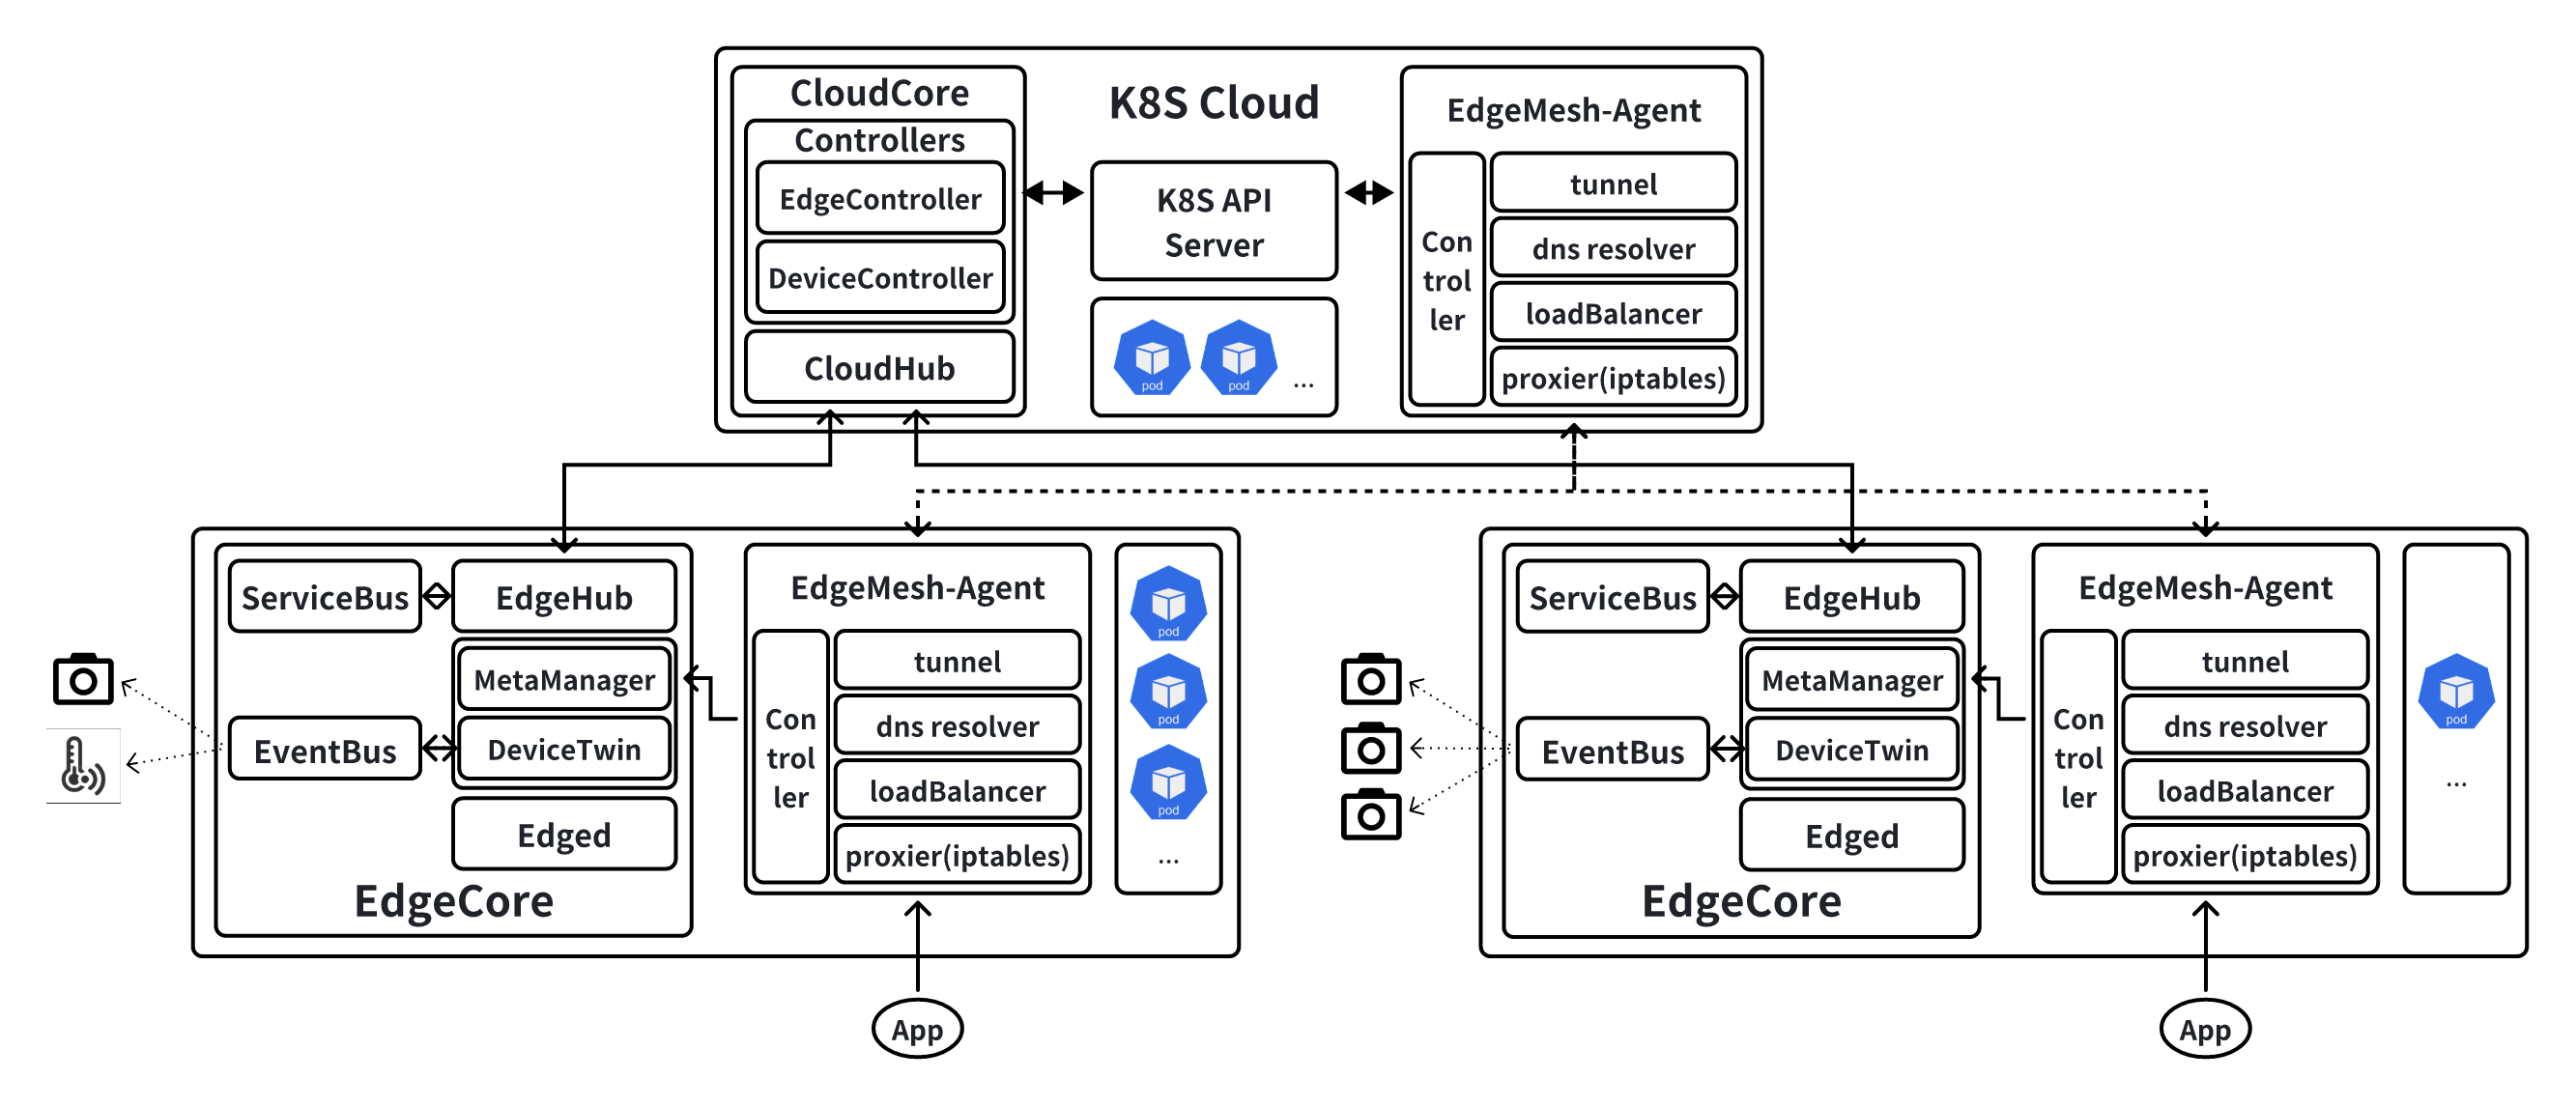
\includegraphics[width=\textwidth]{pics/4-1kubeedge.png}
  \caption{KubeEdge系统架构\cite{xiong2018extend}}
  \label{fig:4-1kubeedge}
\end{figure}

% \begin{figure}[ht]
%   \centering
%   \begin{adjustbox}{center, max width=1.2\textwidth}
%     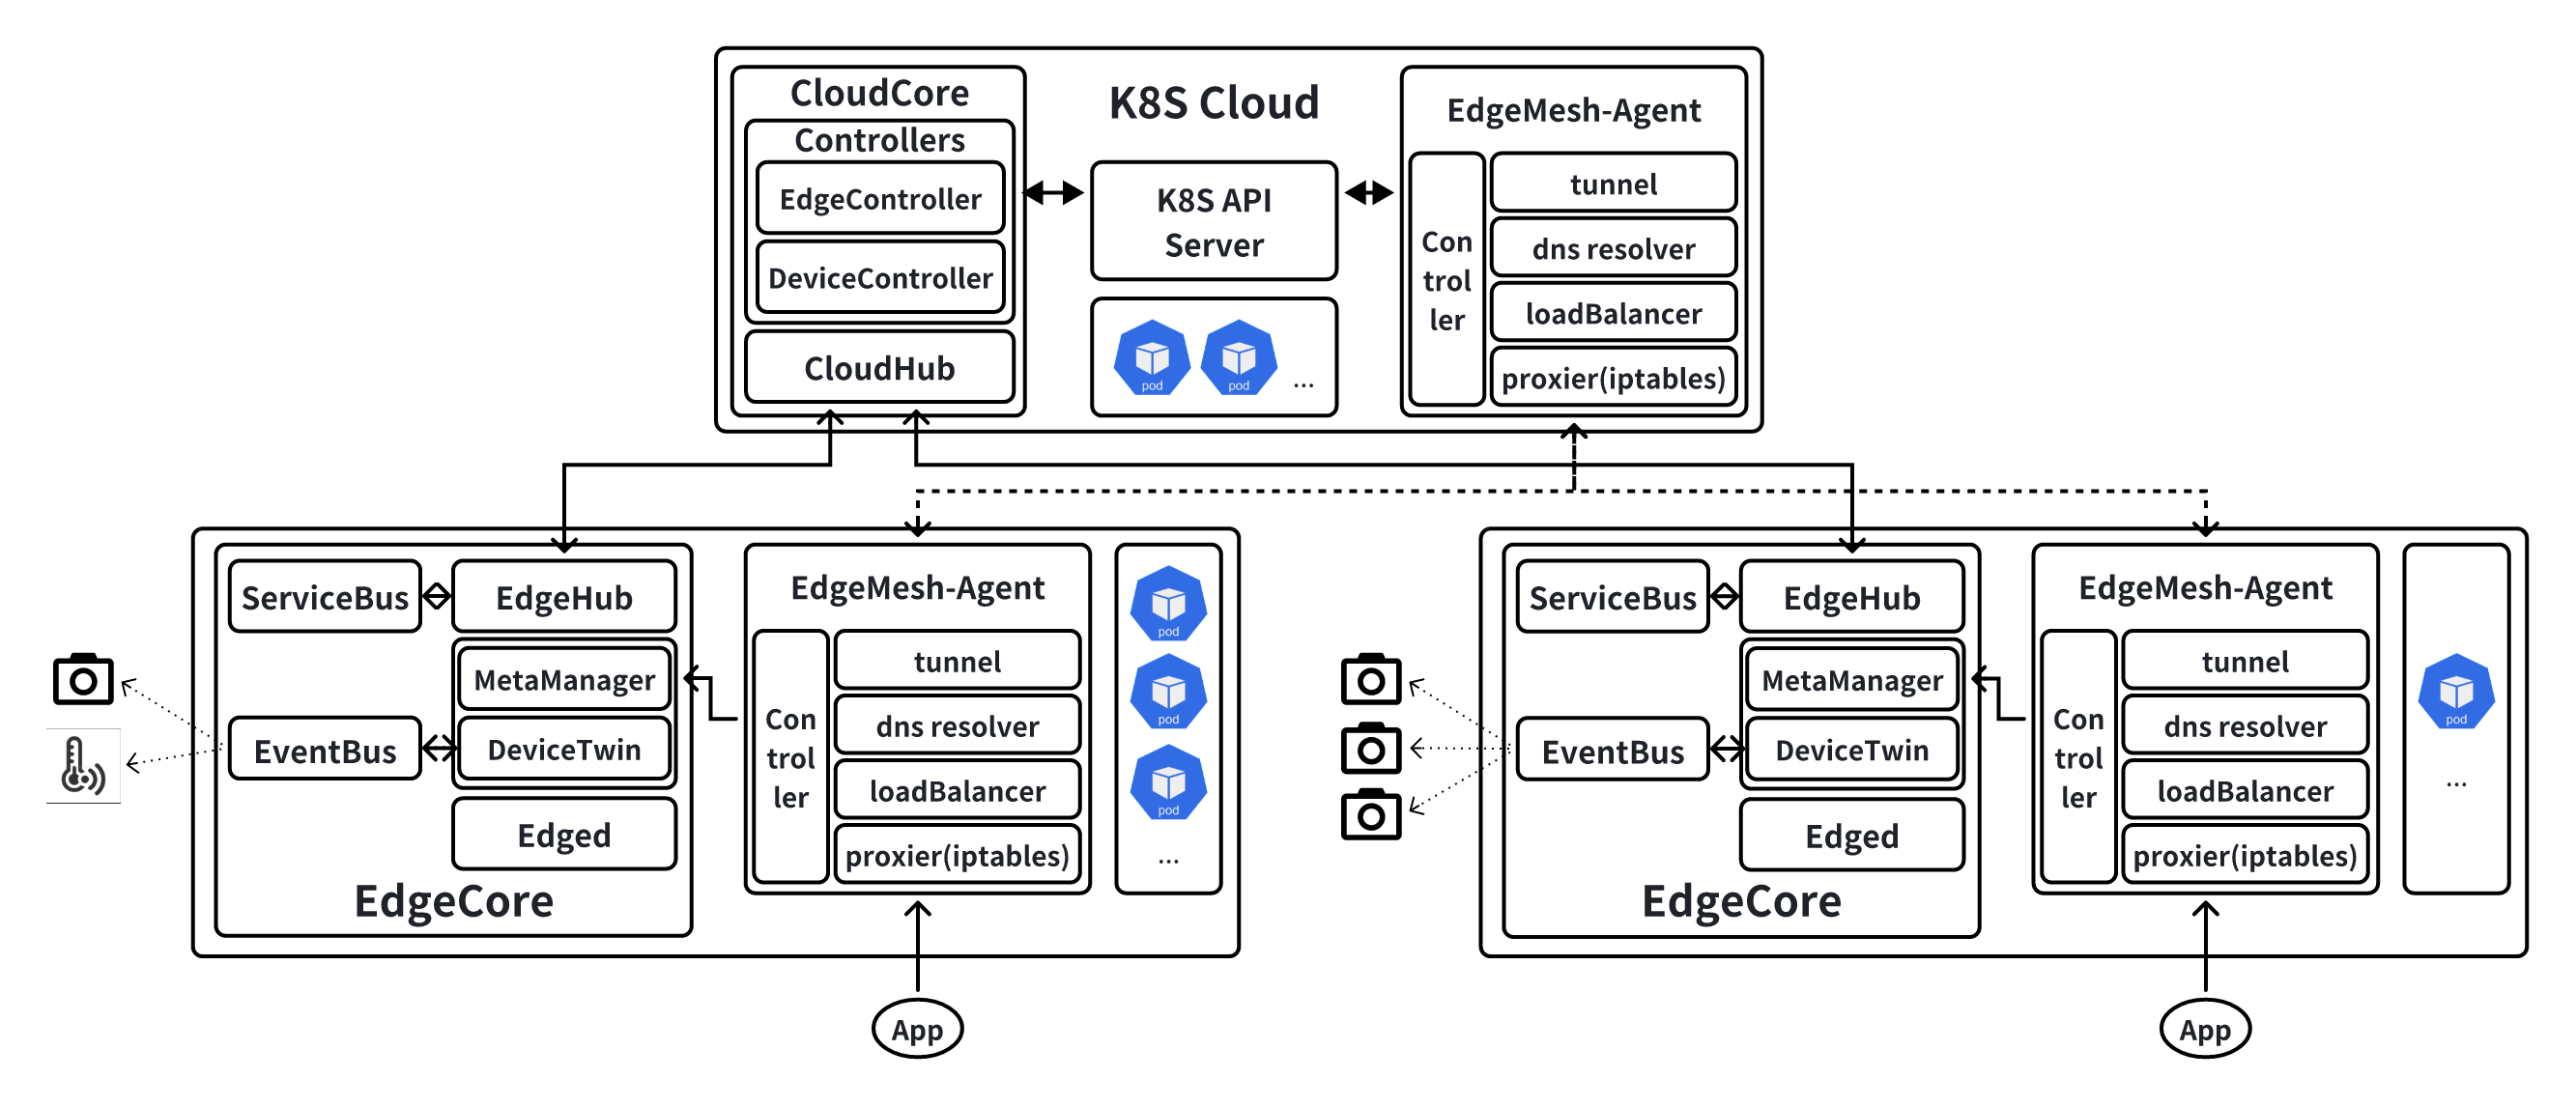
\includegraphics{pics/4-1kubeedge.png}
%   \end{adjustbox}
%   \caption{KubeEdge系统架构\cite{xiong2018extend}}
%   \label{fig:4-1kubeedge}
% \end{figure}


KubeEdge的核心功能依赖于云端和边缘组件的协同工作。云端的边缘控制器(Edge Controller)与边缘侧的EdgeHub组件共同实现了基于事件驱动的双向同步机制。这一机制通过 Kubernetes API Server 与 EdgeCore 的交互,确保了云边节点的状态一致性,同时支持边缘节点注册、服务部署及资源状态的实时更新。此外,CloudHub 和 EdgeHub 组件通过双向 WebSocket 连接构建了分布式消息总机,采用消息缓存与断点续传技术,有效应对网络波动带来的挑战,从而保证通信的可靠性。

在边缘端,KubeEdge通过EdgeD和MetaManager共同支撑轻量化的计算基础设施。EdgeD作为核心执行引擎,深度集成容器运行时接口(CRI),实现了对Pod工作负载的全生命周期管理,涵盖资源调度、机密注入及健康监测等关键功能。MetaManager则作为EdgeD的辅助模块,负责元数据的存储与检索。两者通过分层缓存策略优化了存储效率与访问性能:高频访问的元数据存储在内存数据库中,低频数据则持久化至SQLite。这种设计使得KubeEdge能够在资源受限的边缘环境中高效运行,同时保持与云原生生态的无缝对接。

KubeEdge的设备管理和服务通信能力是其另外两项重要特性,将在后续章节中详细阐述。

\subsection{设备管理模块}

KubeEdge的设备管理模块通过数字孪生技术实现物理设备与虚拟对象的双向映射。如图\ref{fig:4-2mapper}所示,设备控制器(Device Controller)基于Kubernetes CRD机制定义设备抽象模型(Device CRDs),通过声明式API实现设备状态的云端声明与边缘同步。该模块与边缘组件DeviceTwin形成闭环:Mapper框架负责设备数据的采集与协议转换,DeviceTwin将采集数据映射为数字孪生体的状态属性并存储于本地数据库,EdgeHub则通过WebSocket通道将设备状态更新同步至云端。

\begin{figure}[ht]
  \centering
  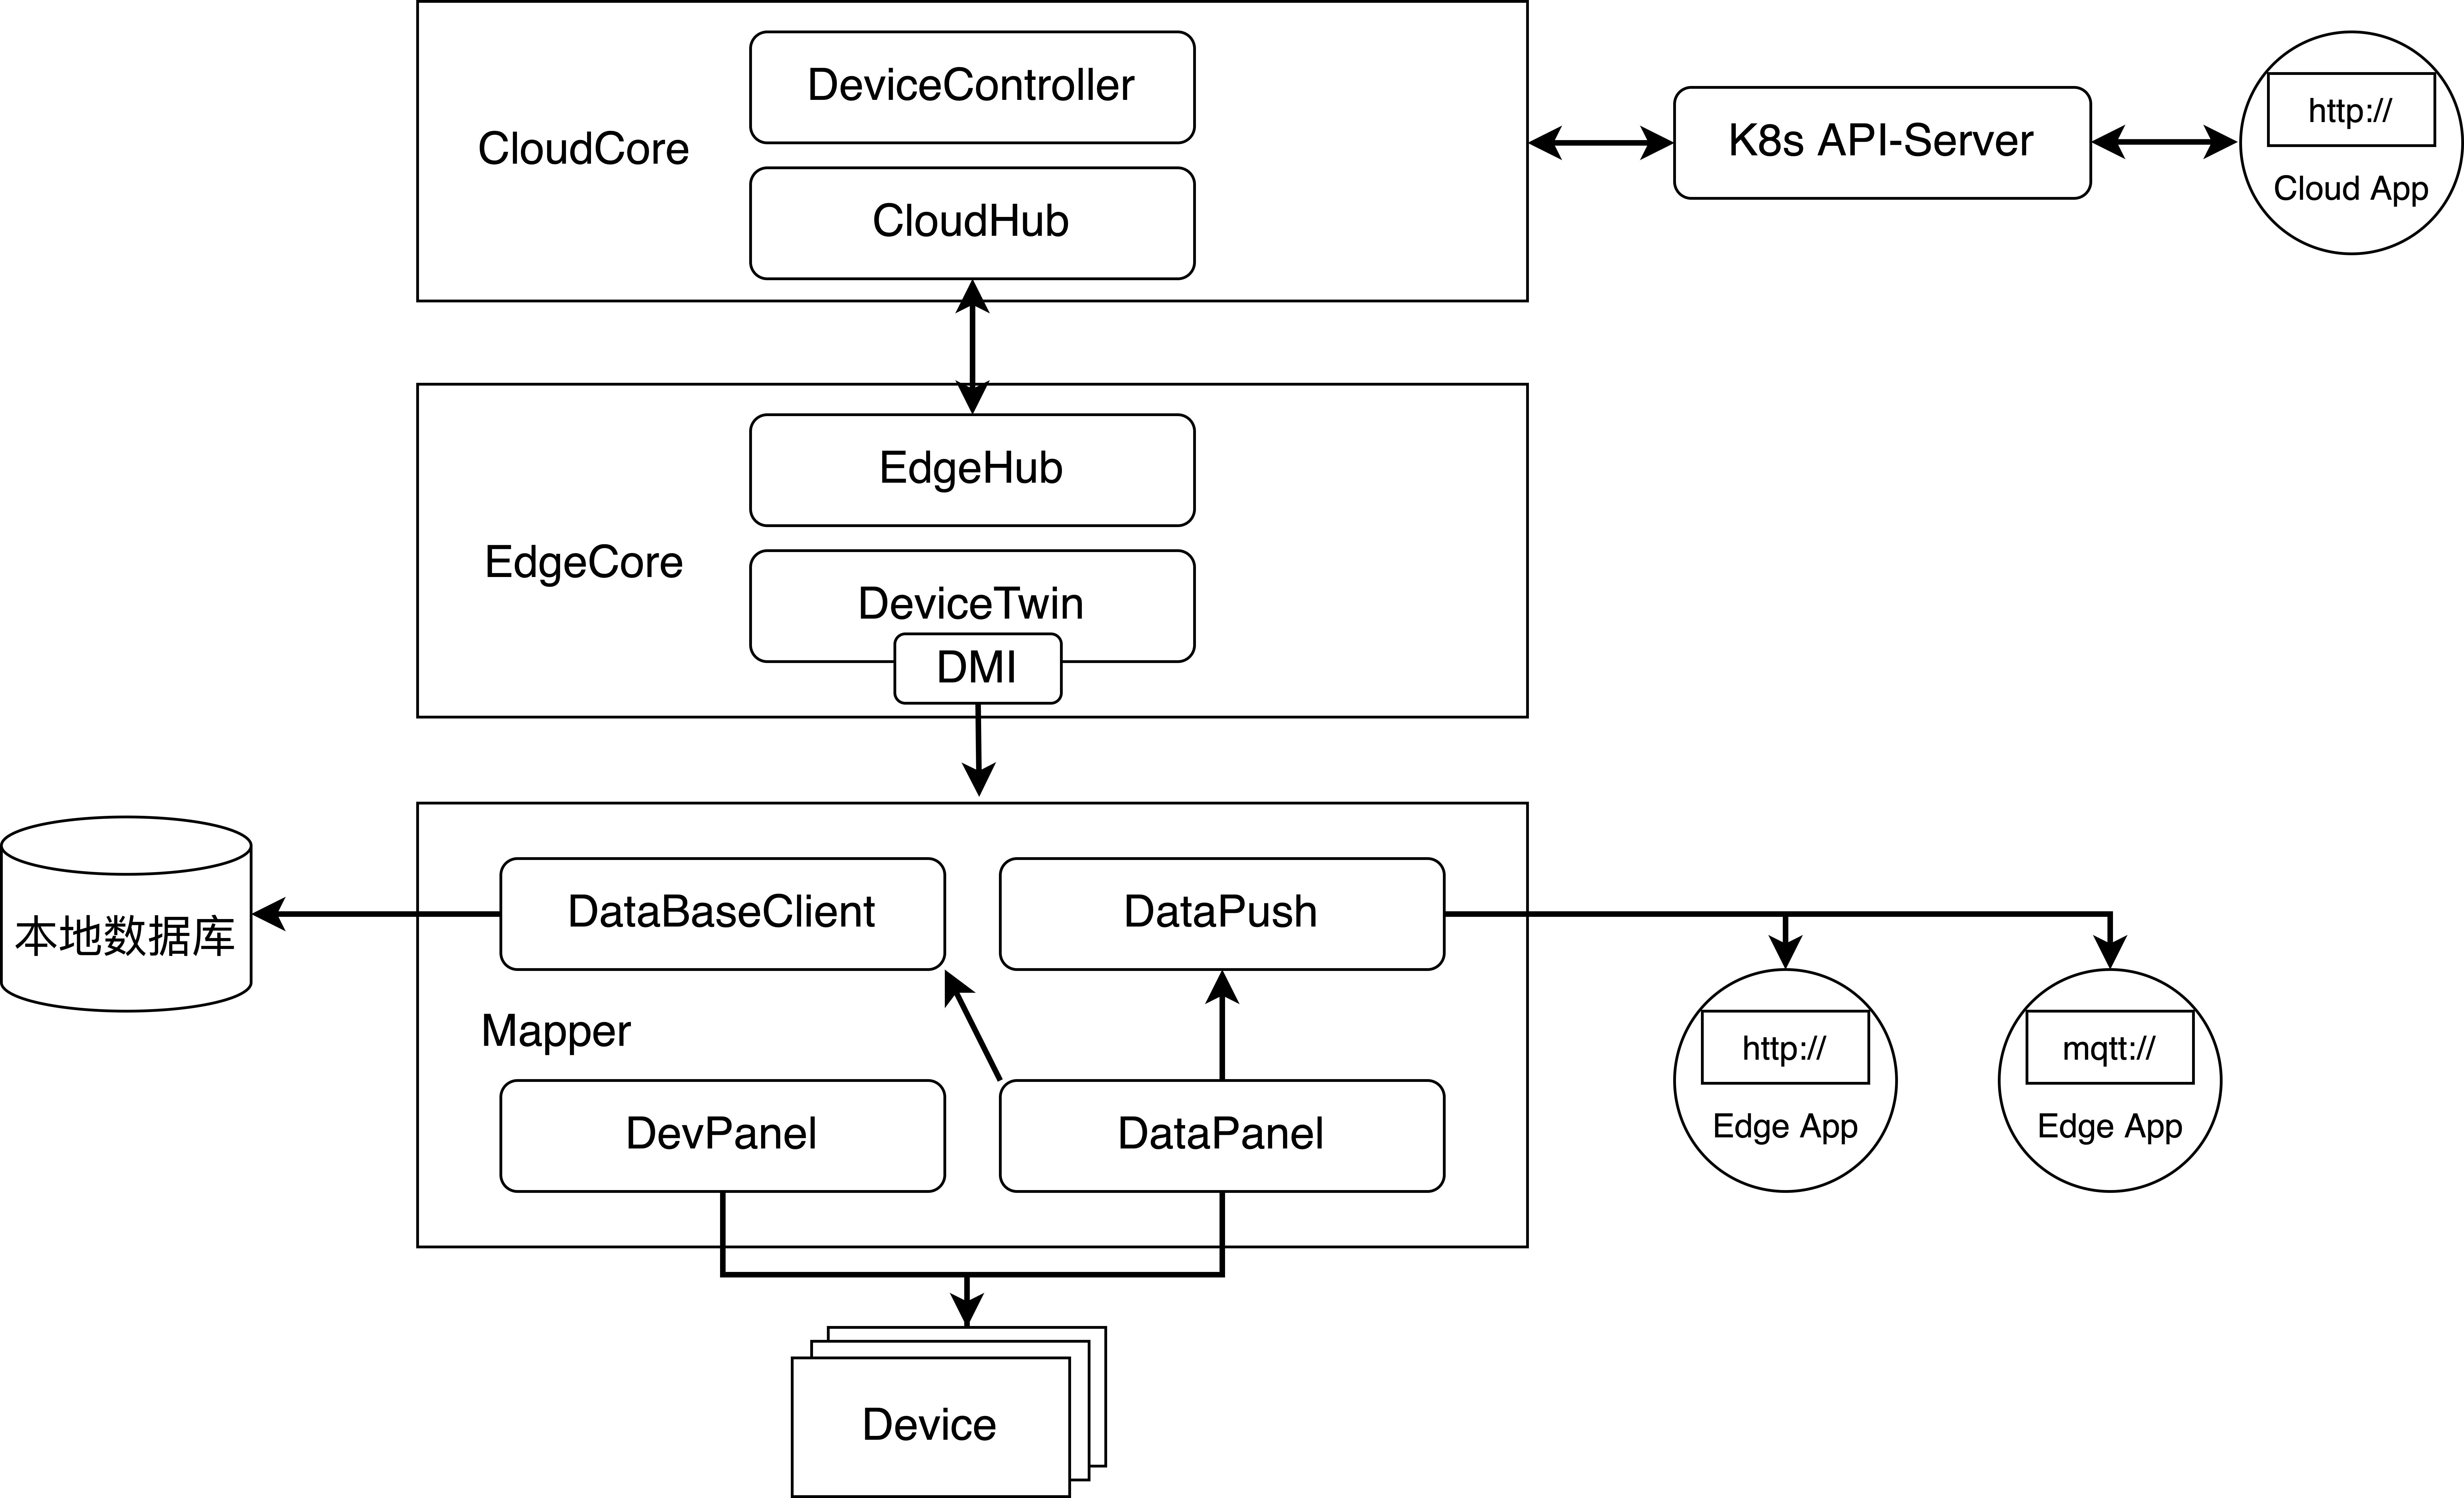
\includegraphics[width=\linewidth]{pics/4-2mapper.png}
  \caption{KubeEdge设备管理架构\cite{xiong2018extend}}
  \label{fig:4-2mapper}
\end{figure}

在 KubeEdge 的设计中,Mapper 框架不仅支持设备平面(DevPanel)的设备运行管理,提供设备数据的采集与协议转换功能,还在数据平面(DataPanel)上提供了灵活的数据推送能力。采集到的设备数据可以通过 MQTT 协议实时推送到消息队列中,以满足实时数据分析的需求;同时,Mapper 还支持将数据推送到时序数据库(如 InfluxDB)中,以便进行高效的时序数据分析与长期存储。这种设计使得KubeEdge能够高效地应对高频率、多源异构的设备数据流,并根据任务需求动态调整数据处理路径,从而实现云边协同中的资源优化与性能提升。

本文利用 KubeEdge 提供的 Device CRDs 和 Mapper 框架模块来管理终端设备。具体而言,Device CRDs 用于描述设备的静态属性和能力,这些属性包括设备的功能特性、通信协议以及数据格式等信息。Mapper 框架则负责实现设备的动态数据采集逻辑,支持根据预定义的采集策略或外部事件触发机制动态调整数据采集行为。

\subsection{基于EdgeMesh的服务通信}

EdgeMesh 是 KubeEdge 集群中用于实现服务发现和跨节点通信的核心组件,其设计目标是解决边缘计算场景下节点间通信的复杂性和不稳定性问题。在边缘计算环境中,网络条件通常受限,尤其是弱网环境下的跨局域网通信需求更为突出。为应对这一挑战,EdgeMesh 基于 LibP2P 技术构建了一套去中心化的通信网络。该网络能够动态适应网络拓扑的变化,从而在边缘节点之间建立高效、可靠的数据传输通道。

在局域网内,EdgeMesh 支持直接访问的方式完成节点间的数据交互;而在跨局域网场景下,EdgeMesh 通过 NAT 打洞技术或中继流量的方式实现节点间的通信。此外,EdgeMesh 借助 EdgeHub - CloudHub 隧道分发元数据,避免了对云端的直接访问,从而显著降低了云端的负载压力。为了进一步提升服务发现的可靠性,EdgeMesh 在每个节点上部署了轻量级的 DNS 服务器。这种设计确保了服务搜索的高效性和准确性,同时支持动态更新和分布式管理。

本文利用 EdgeMesh 的服务发现功能和跨节点通信能力,实现了节点之间调度模块的高效通信。具体而言,EdgeMesh 的去中心化通信网络为跨节点的调度决策提供了低延迟、高可靠的数据传输通道。此外,EdgeMesh 的服务发现机制通过轻量级 DNS 服务器的支持,为流式数据的转发提供了支撑,使其在边缘节点间的高效传递。

\begin{figure}[ht]
  \centering
  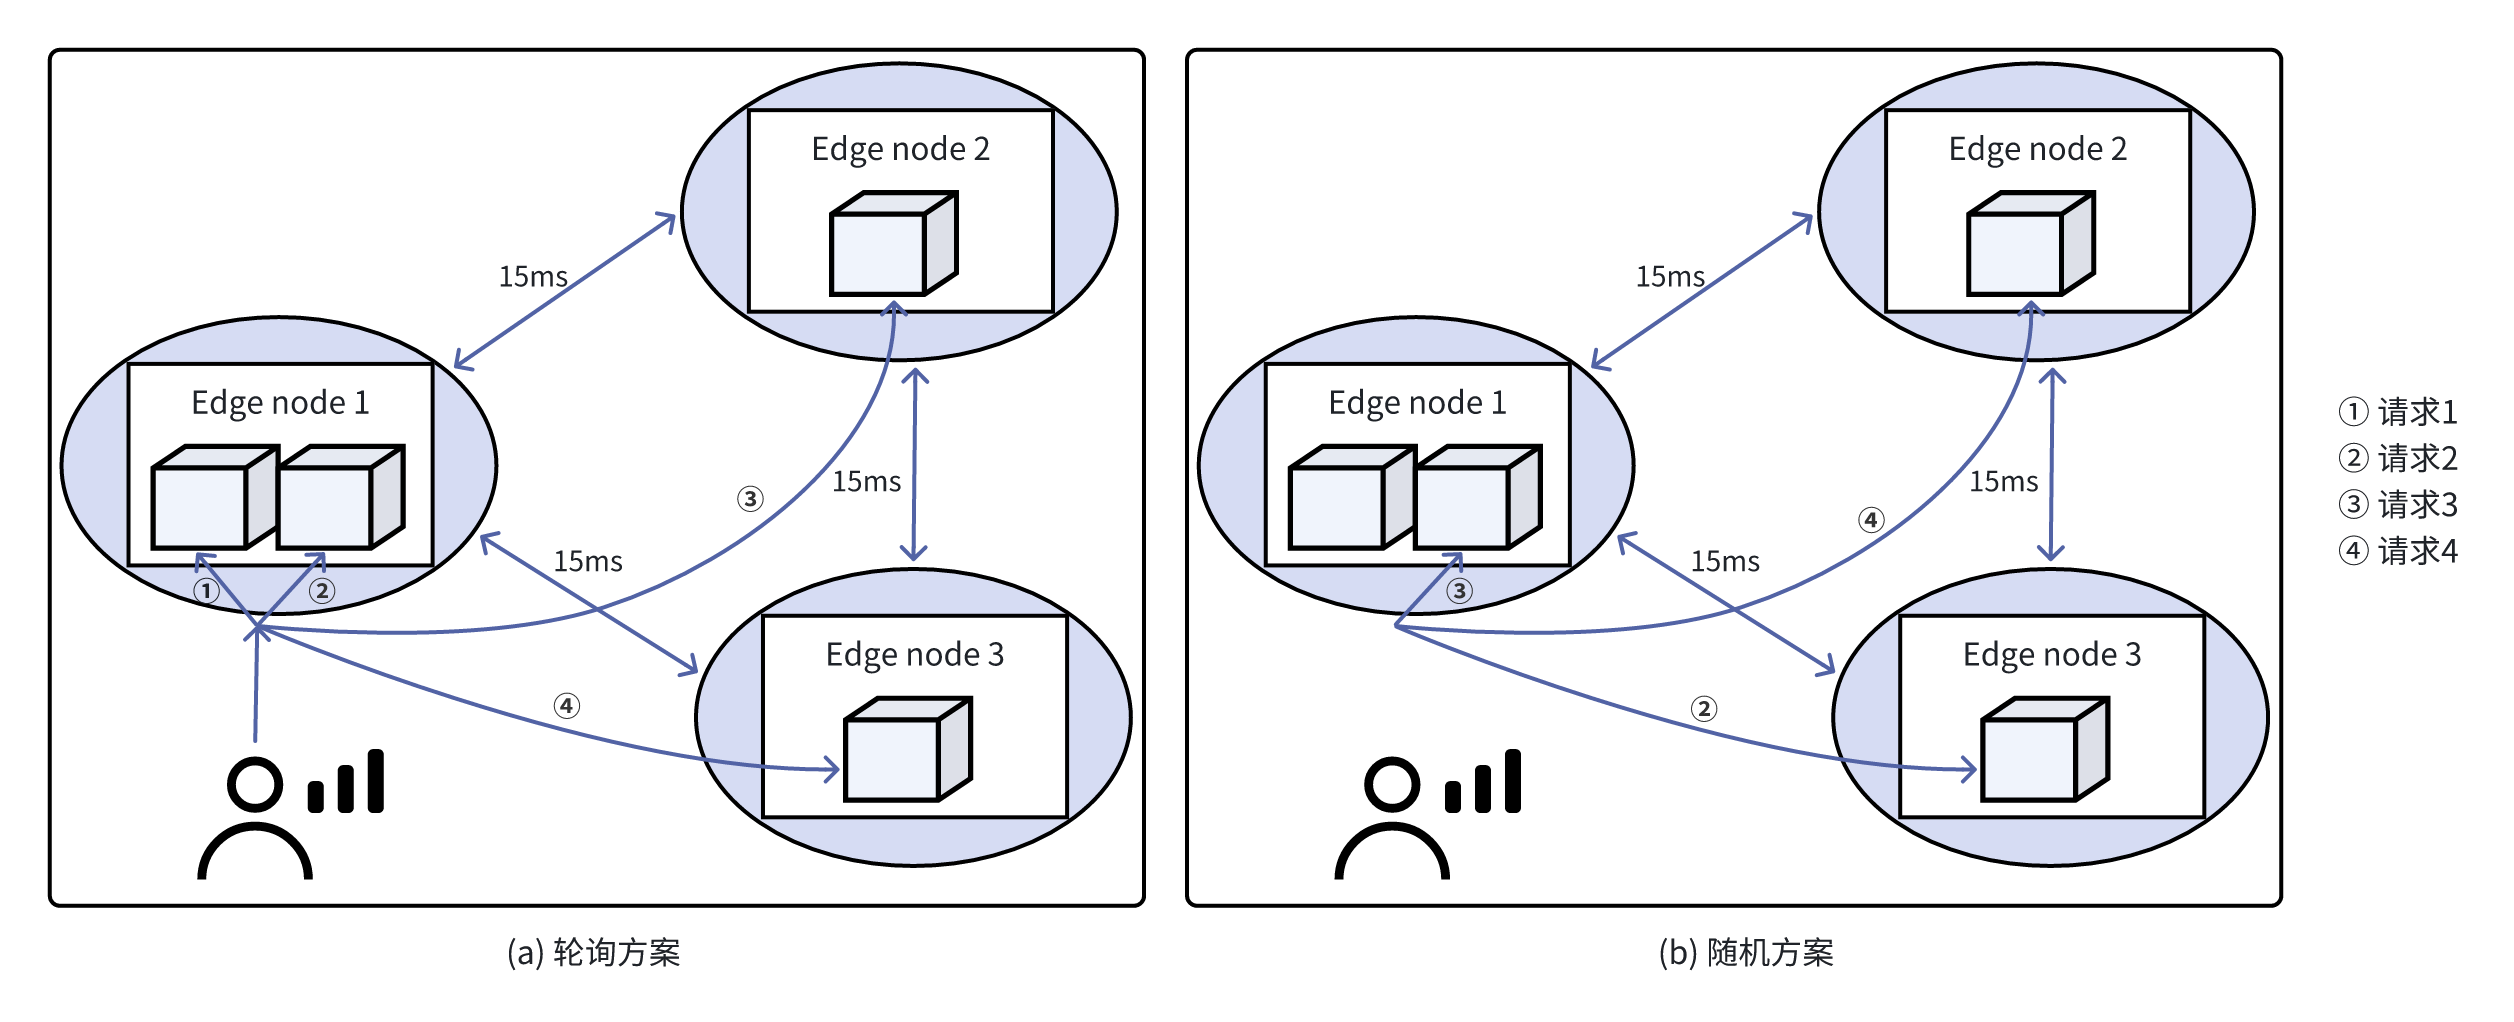
\includegraphics[width=\linewidth]{pics/4-3edgemesh.png}
  \caption{KubeEdge 中的负载均衡方案}
  \label{fig:4-3edgemesh}
\end{figure}

在负载均衡方面,EdgeMesh 目前采用 Istio 的目标规则(DestinationRule),并支持轮询和随机分配等基础策略,以实现流量在各 Pod 间的高效分发,如图 \ref{fig:4-3edgemesh} 所示。然而,在云边协同 AI 推理场景中,边缘节点分布广、网络异构性高,这种传统的负载均衡方式因未考虑节点实时负载、网络质量差异及资源异构性,可能导致任务分配不均或资源利用率低下。

\section{系统架构设计}

在第三章的基础上,本文提出了一种基于 KubeEdge 的原型系统 KEAS。该系统的核心在于实现了分层的调度机制。为支持这一复杂的调度机制,KEAS 在 KubeEdge 平台上构建了一个 Akka 集群,并在物理的三层拓扑上构建了分层的逻辑拓扑,以实现高效的调度管理。同时,利用 Akka Actor 模型实现设备数据流请求的高效转发与模块间通信。Actor 模型通过异步消息传递机制避免了传统多线程编程中的锁竞争问题,从而显著提升了系统的并发性能和可靠性。此外,其异步通信特性能够有效应对云边协同场景中网络延迟和不稳定的问题,确保消息传递的可靠性和低延迟。为实现 Akka 集群与 KubeEdge 的深度集成,本文设计了监听协调模块。该模块通过 Kubernetes 的 Informer 机制实时监控集群状态,并调用 Kubernetes API 动态部署和管理关键负载。

\begin{figure}[ht]
  \centering
  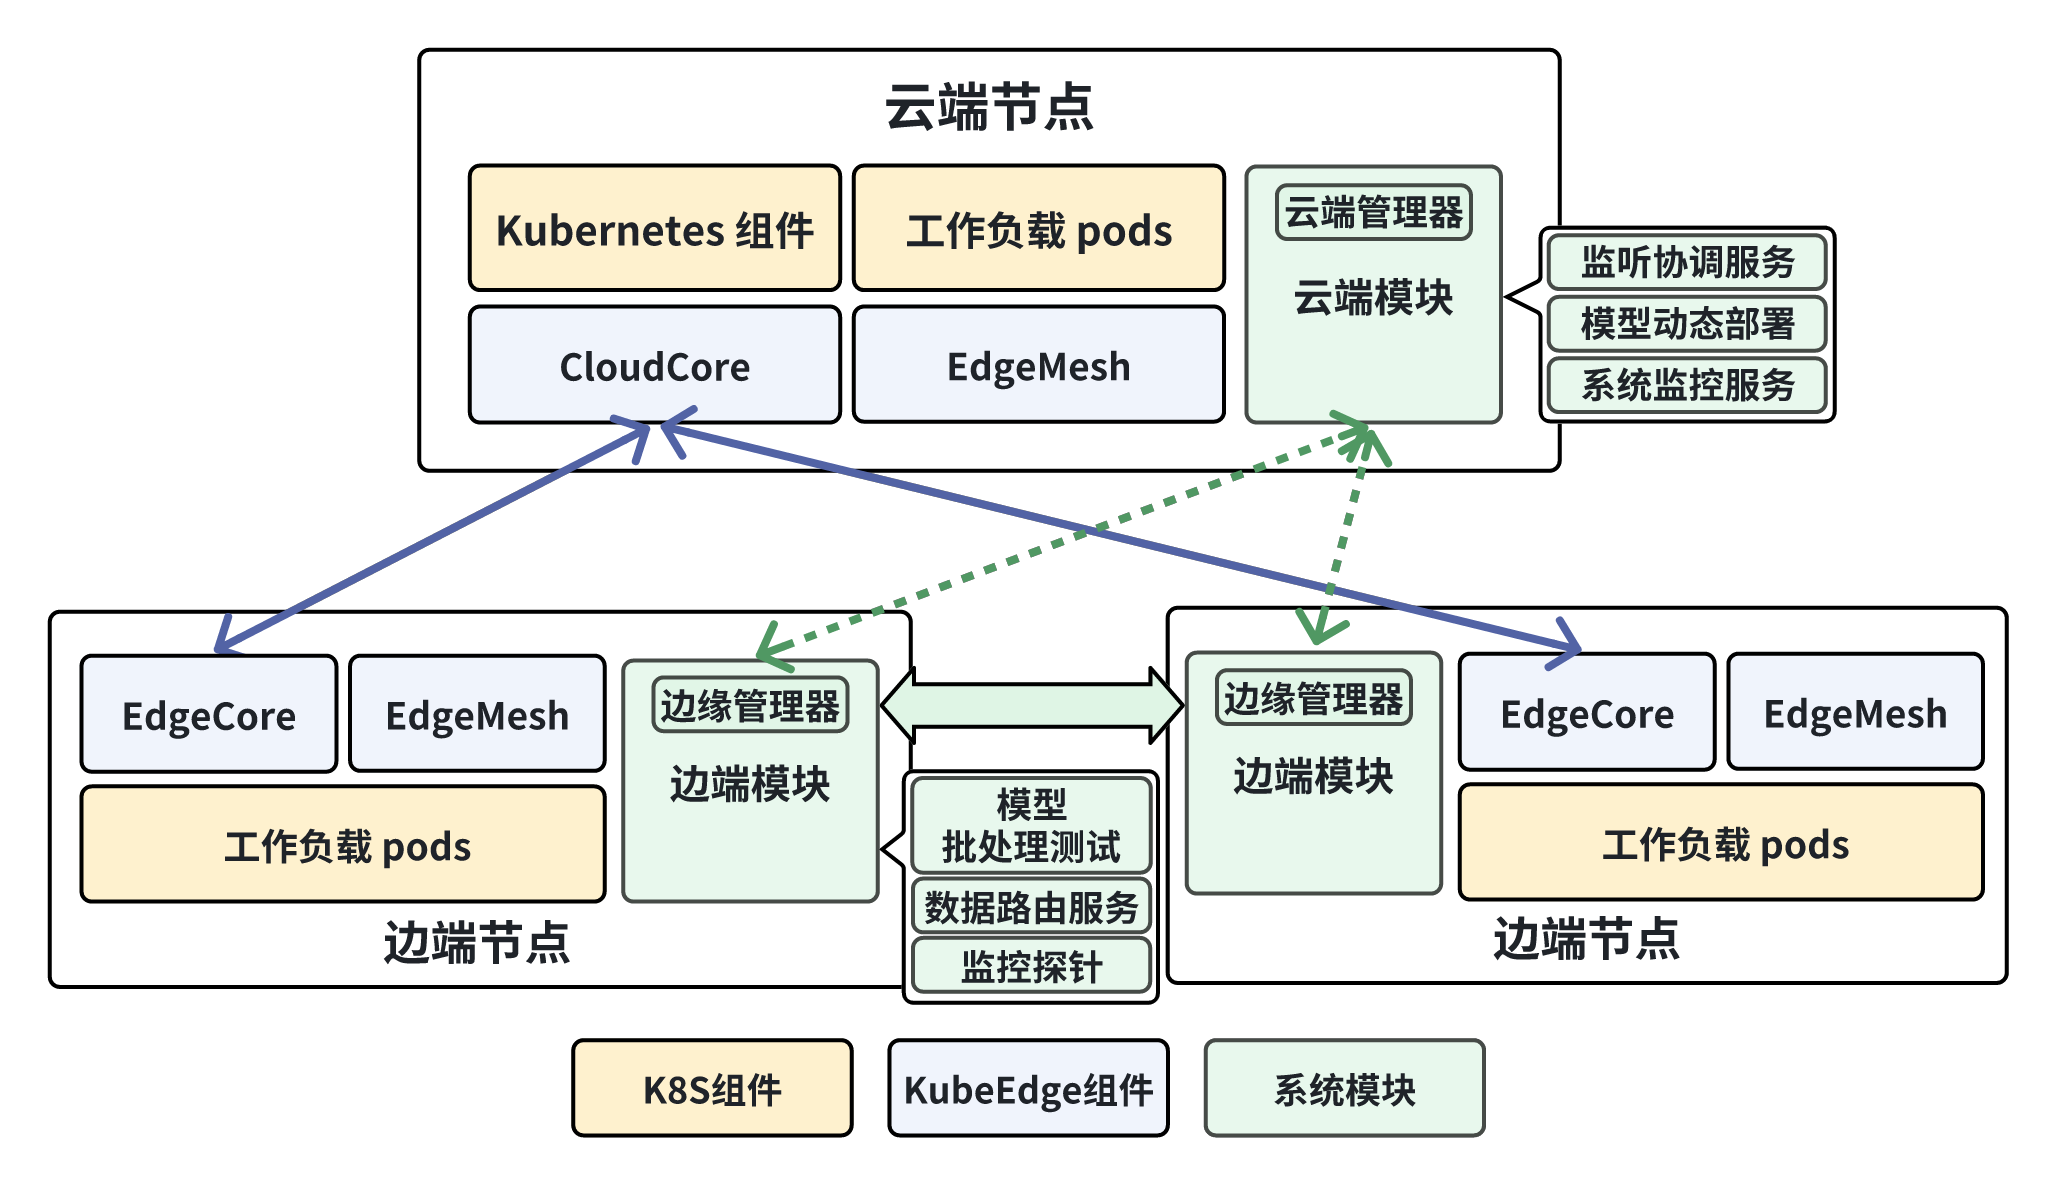
\includegraphics[width=\linewidth]{pics/4-4系统架构.png}
  \caption{KEAS 系统架构}
  \label{fig:4-4arch}
\end{figure}

系统的整体架构如图 \ref{fig:4-4arch} 所示。KEAS 系统首先需要在异构化节点上部署 AI 模型,并针对不同节点的计算能力优化模型运行参数。为此,本文引入了一个AI模型批处理测试模块,在 AI 模型部署阶段对节点进行性能评估。该模块通过测试不同批处理大小下的AI模型推理性能,记录每个节点在处理特定负载时的最优批处理大小及对应的运行时间。这些数据为后续调度策略的制定提供了重要依据。同时,系统通过监控探针实时采集集群节点之间的网络状况和节点运行状态。在云端,系统监控模块汇总并展示每个节点的运行状态以及节点间的网络通信情况,为调度决策提供全面的数据支持。基于上述数据采集与分析,KEAS 系统实现了分层调度策略的关键数据输入。针对调度结果,边端模块进一步实现了数据流转发路由功能,将设备流式数据高效地转发至相关节点进行处理。

具体而言,系统中的关键组件包括:

\begin{itemize}
    \item \textbf{基于 Akka 的调度服务:} 该服务基于Akka Cluster构建的核心调度模块,由云端管理器(Master)和边缘管理器(Manager)组成,支持云端全局调度和边缘节点的分层调度。云端管理器负责执行全局调度策略和动态部署模型推理实例,同时维护节点运行状态与全局网络信息,为系统提供统一的调度视图和全局资源管理能力。边缘管理器则部署在边缘节点上,主要职责是高效调度本地任务;此外,边缘管理器还能根据用户需求动态组建分层结构,实现边缘节点间的协同管理和资源优化利用。
    \item \textbf{监听协调服务:} 该服务的核心功能是实现 Kubernetes 集群中的资源感知与动态部署。该服务利用 Kubernetes 的 Informer 机制,实时捕获设备状态和集群原生资源的变更信息,并根据这些信息触发相应的记录或调度操作。例如,在节点加入集群时,系统会记录其架构信息;当设备状态发生更新时,可能触发调度流程以适应新的资源环境。此外,核心资源部署机制通过预置的标准化部署模板,自动化完成负载实例的创建、配置与管理,从而显著简化了云边协同环境中复杂的资源调度与部署任务。
    \item \textbf{模型推理服务:} 该服务聚焦于推理部署环节,有效解决了模型跨框架兼容性、硬件异构性以及动态部署等关键问题。具体而言,通过预先为不同硬件架构打包适配的推理服务镜像,并结合 Kubernetes 的节点标签机制,确保镜像与目标节点的兼容性。同时,设计了模型转换模块,支持不同框架之间的模型相互转换。在完成模型实例的动态部署后,系统通过批处理测试对推理性能进行优化,并记录批处理大小和单次运行时间等相关数据,为后续调度服务提供可靠的数据支持。
    \item \textbf{数据路由服务:} 该服务是实现高效数据分发与处理的核心组件,通过订阅 MQTT 消息代理获取设备数据,并依据调度服务生成的路由规则确定数据流向。数据会被传递至本地模型推理实例以完成后续处理,或者在需要时转发至其他节点的 MQTT 消息代理,从而实现跨节点的数据流转。
    \item \textbf{系统监控服务:} 该服务提供全面的监控功能,包括网络监控和队列监控,实时采集节点间的网络状况和节点运行状态,为调度决策提供数据支持。监控服务通过可视化界面展示集群的运行状态,帮助相关人员快速定位问题并优化资源配置。
\end{itemize}

\section{系统组件设计}

\subsection{基于 Akka 的调度服务}

在本系统中,终端设备的数据采集任务已由 KubeEdge 平台完成。为了实现分布式节点之间的状态同步以及高效的任务分发,本文在 KubeEdge 平台上构建了一个基于 Akka Cluster 的分布式调度服务。该调度服务不仅作为系统的核心调度组件,还承担了运行时状态管理与消息传递等关键职责,是整个系统的基础架构。

\begin{figure}[ht]
  \centering
  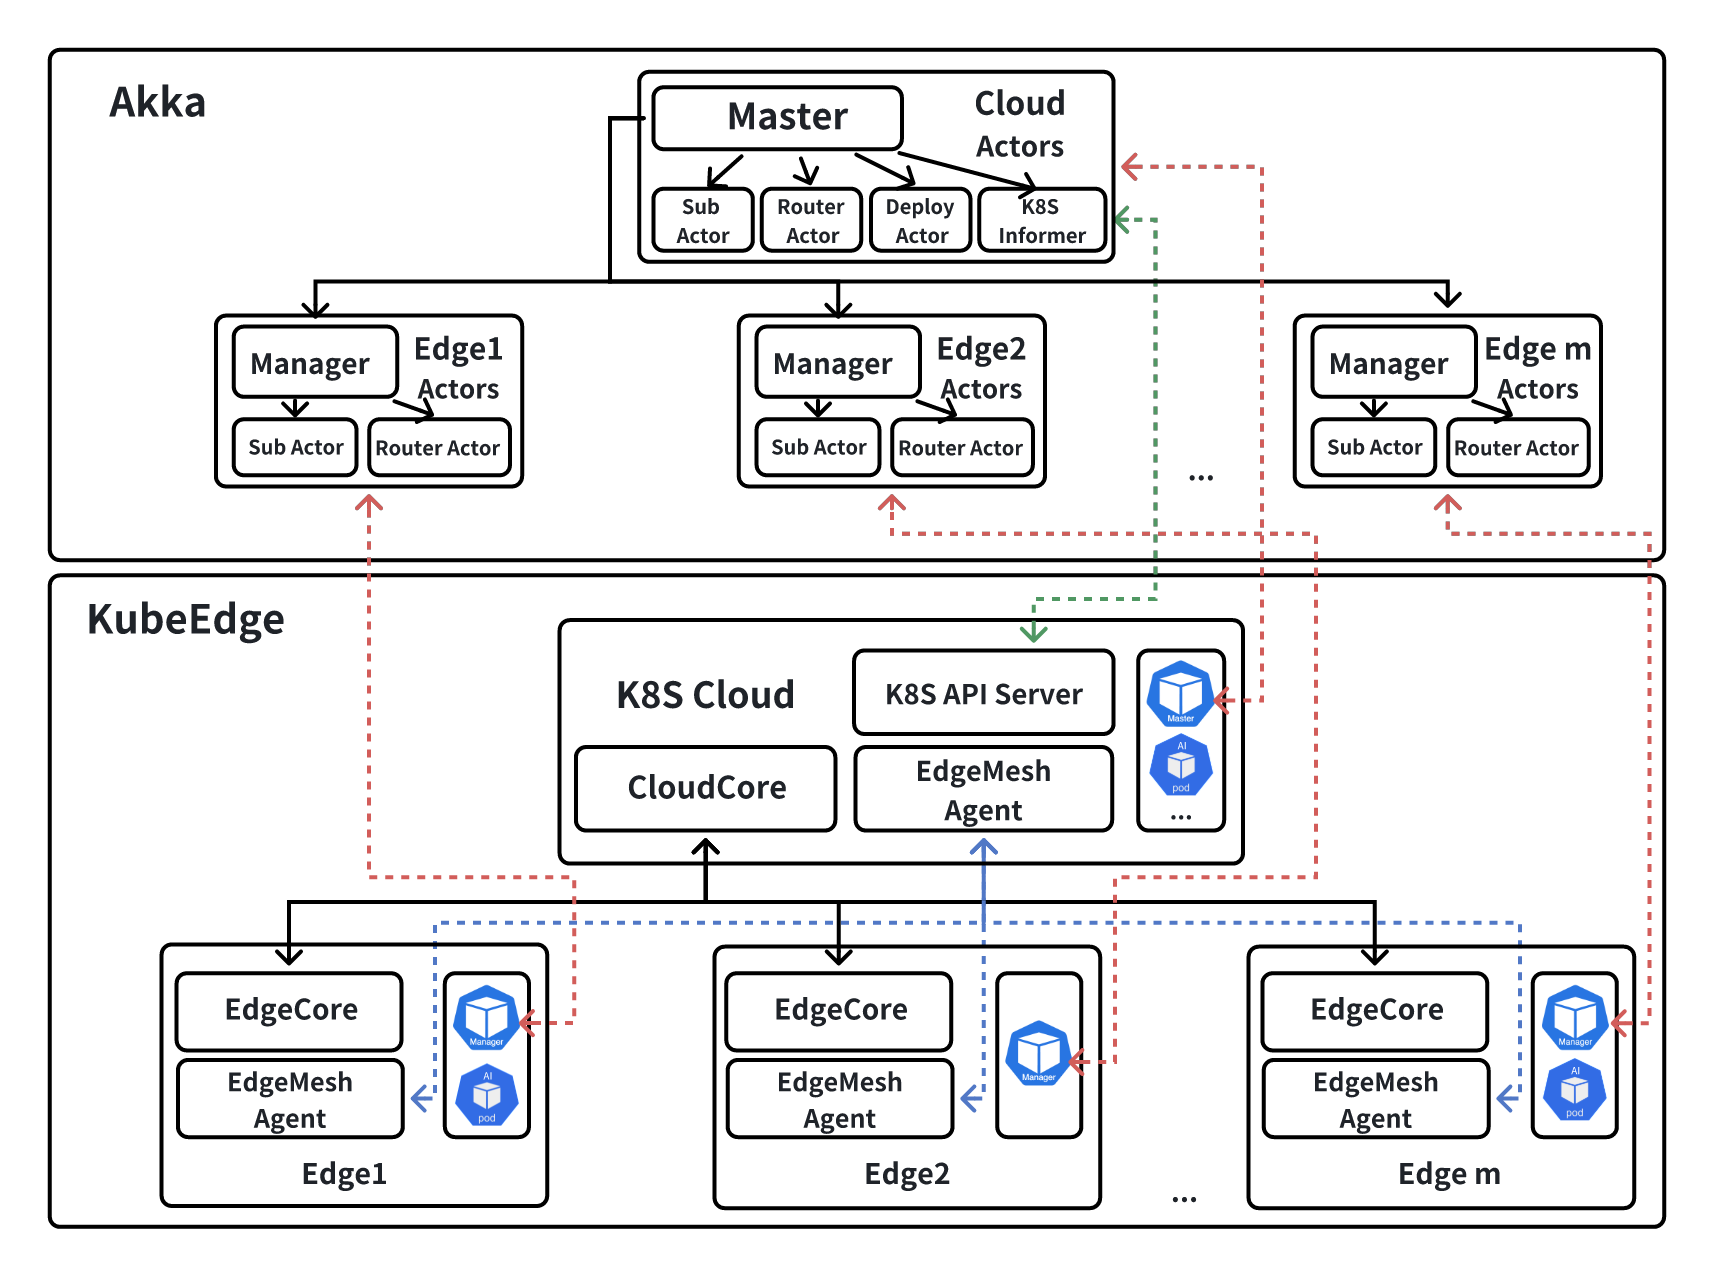
\includegraphics[width=\linewidth]{pics/4-5akka.png}
  \caption{基于 Akka 的调度服务架构}
  \label{fig:4-5akka}
\end{figure}

如图 \ref{fig:4-5akka} 所示,Akka 集群架构主要由云端管理器(Master)和边缘管理器(Manager)组成,两者通过 Akka Cluster 连接。云端管理器部署于云端节点,承担全局调度策略的执行职责。它不仅需要维护各节点上模型推理实例的运行状态,还需掌握全局网络信息。具体而言,运行状态涵盖批处理大小、单次运行时长及队列长度等关键指标。这些数据为第三章所述调度算法在云端层次的应用提供了基础支持。此外,云端管理器还负责动态部署模型推理实例,该过程将在后续章节关于监听协调服务与模型推理实例动态部署的部分中进一步探讨。

\begin{figure}[ht]
  \centering
  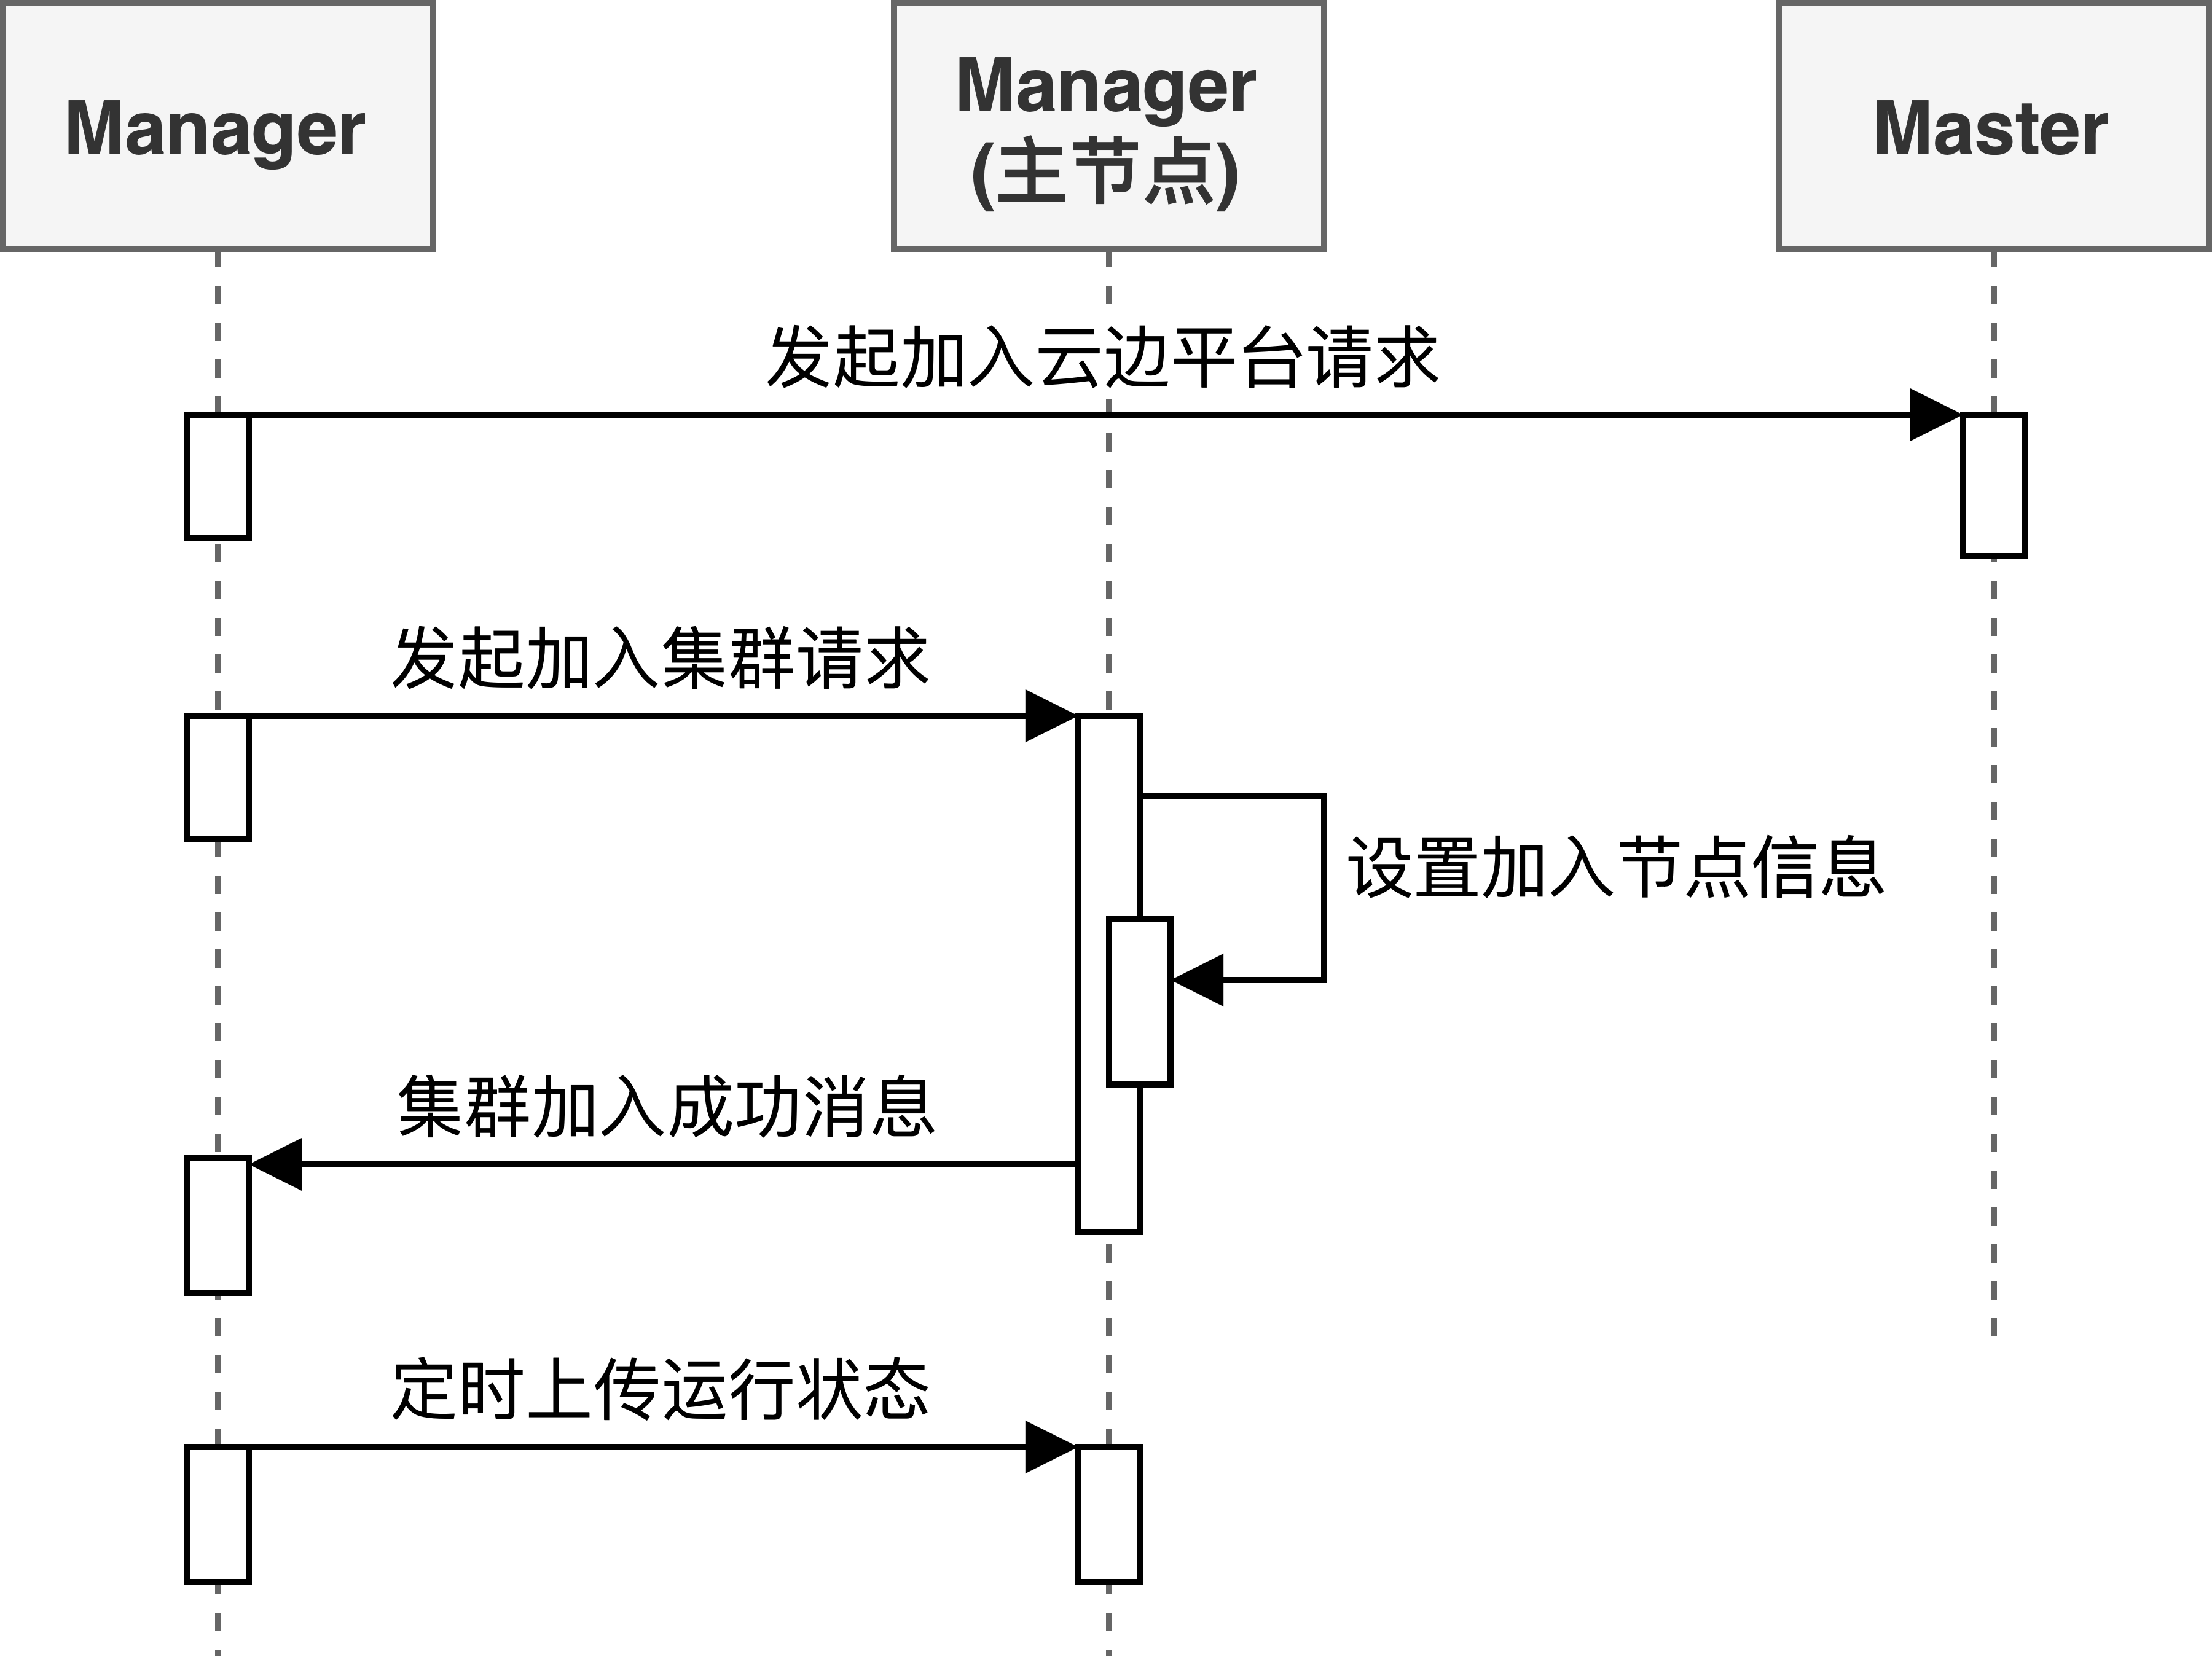
\includegraphics[width=0.7\linewidth]{pics/4-6集群加入.png}
  \caption{新节点加入边缘集群的时序图}
  \label{fig:4-6join}
\end{figure}

边缘管理器(Manager)部署在边缘节点上,主要负责本地任务的调度与资源管理。多个边缘管理器可以组成树状逻辑拓扑结构,每个子树可视为一个边缘集群,其中根节点即为该集群的主节点,承担整个集群的任务调度职责。当有新的边缘节点需要加入集群时,用户需根据实际场景指定一个已属于目标集群的节点作为初始接入点。例如,在实际部署中,用户可以选择与新节点处于同一局域网或同一地理区域的任意一个集群节点作为接入点。如图 \ref{fig:4-6join} 所示,新节点首先通过 Akka Cluster 机制向云端管理器发送加入云边平台的请求。如果用户指定了加入的目标边缘节点,则新节点会向该指定节点发送加入集群的请求消息。这个指定的节点将成为新节点的主节点,并负责配置新节点的相关信息。一旦主节点完成配置,它会返回集群加入成功的消息给新节点。此时,新节点也会设置主节点的信息,并开始定时上报自身的运行状态。

\begin{figure}[ht]
  \centering
  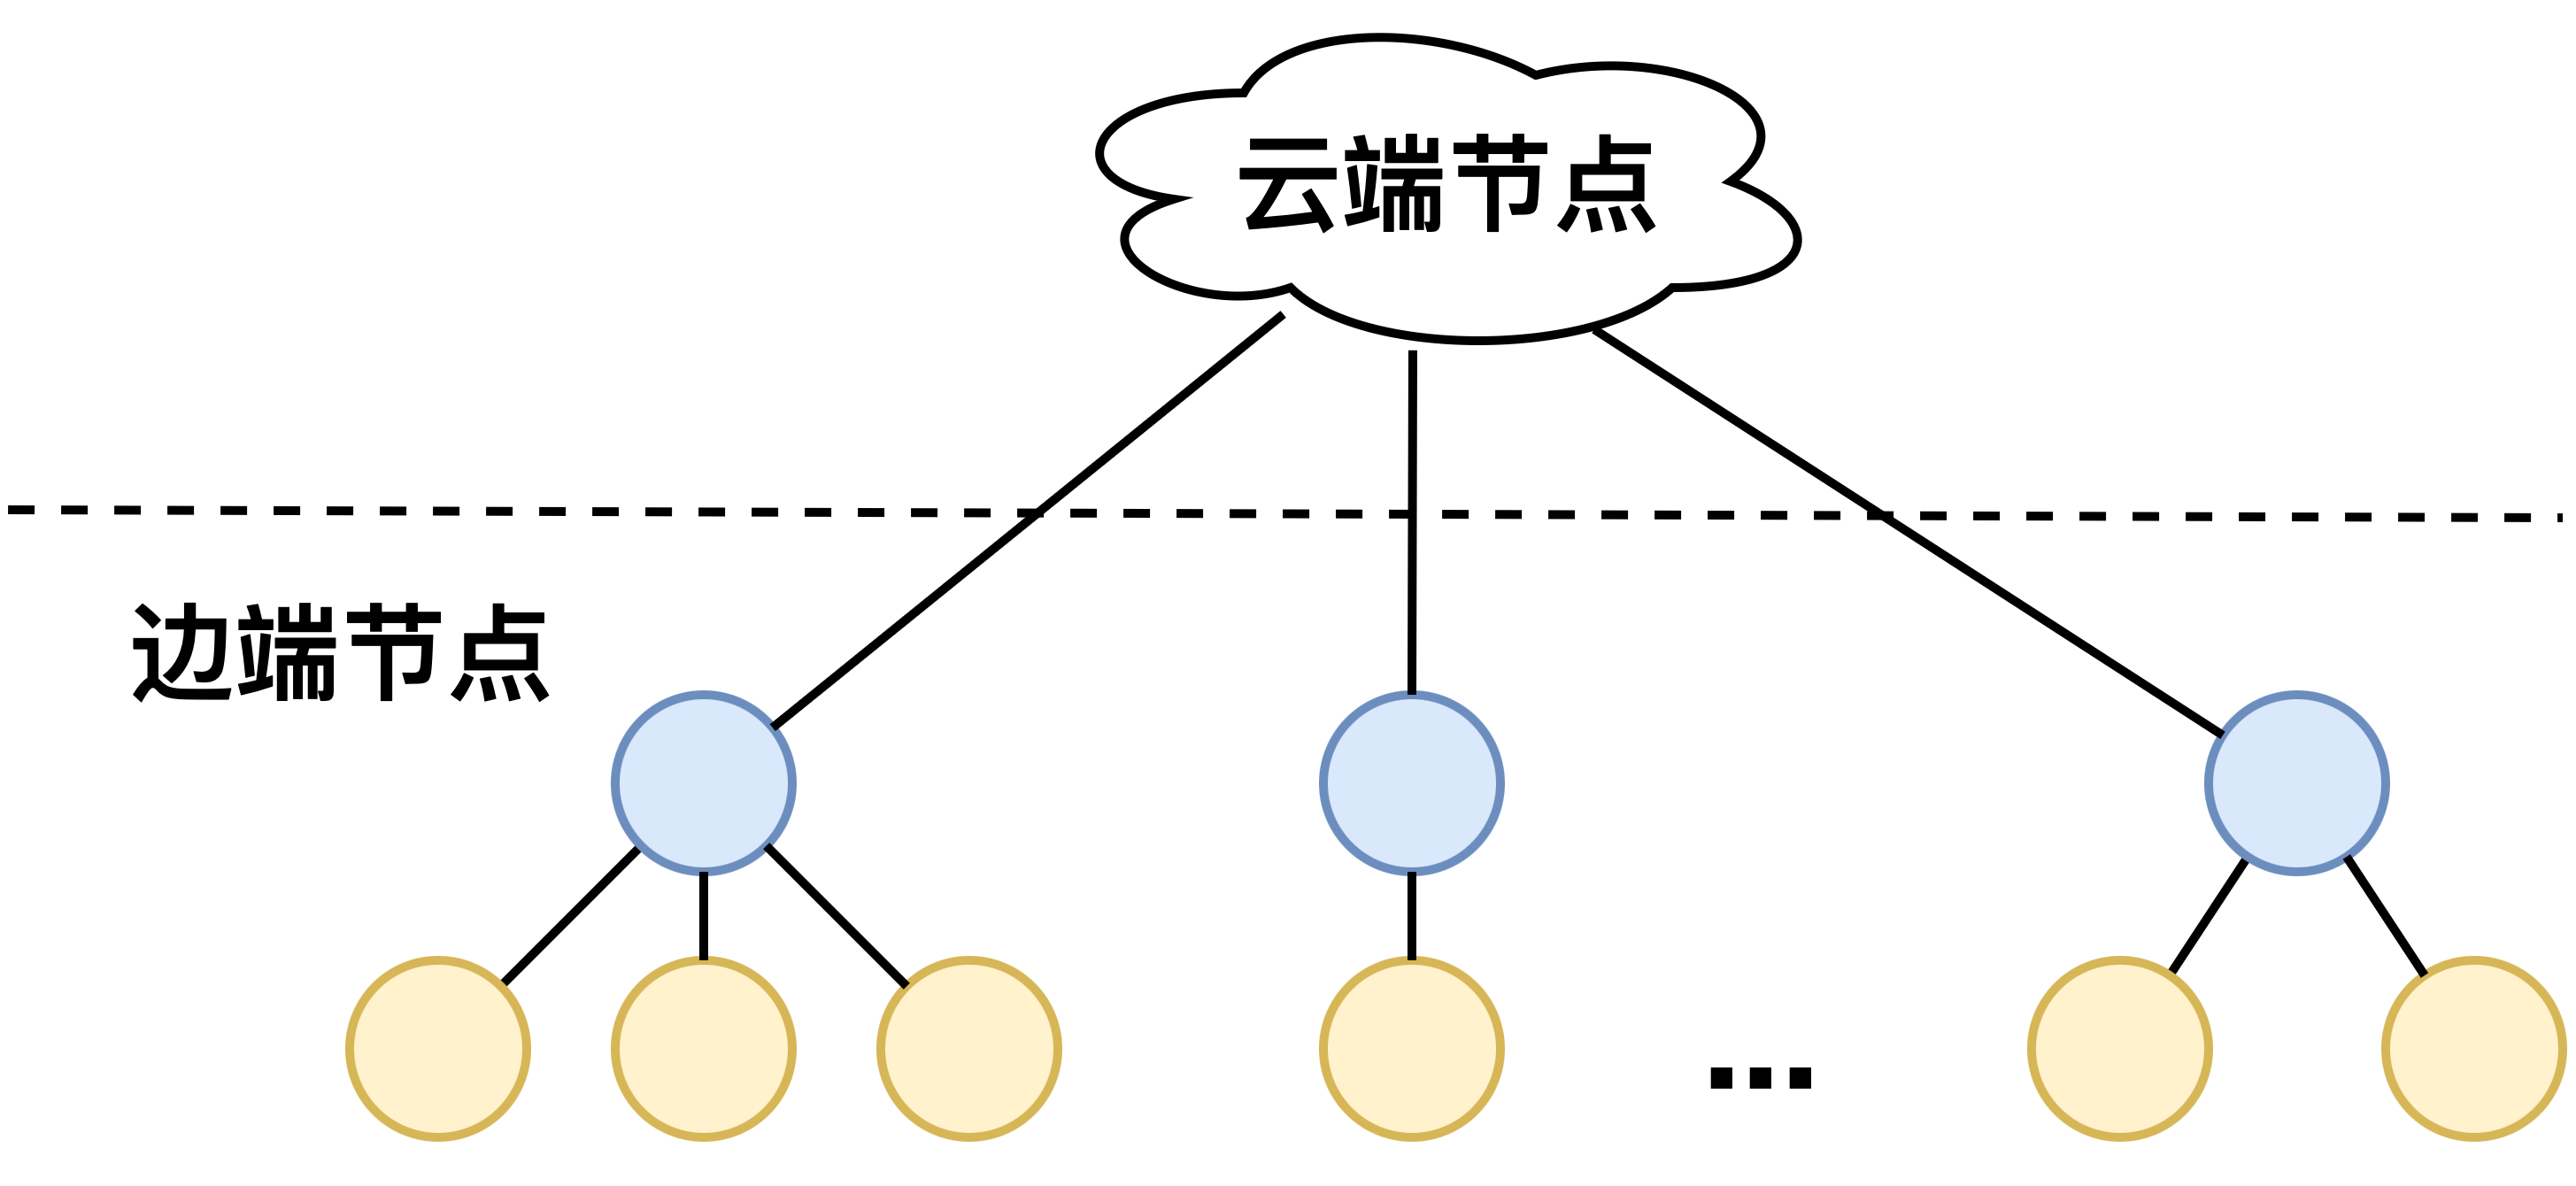
\includegraphics[width=0.6\linewidth]{pics/4-5arc.png}
  \caption{云边拓扑结构}
  \label{fig:4-5arc}
\end{figure}

通过这种方式,本文实现了边缘节点之间的树状逻辑拓扑结构。为了简化论述,本文假设边端节点配置为两层结构,即直接连接设备的节点和集群的主节点,如图 \ref{fig:4-5arc} 所示。这种两层结构不仅便于理解,而且可以轻松扩展到多层结构,当某一层的调度失败时,任务可以自动向上一层进行调度,从而实现高效的资源利用和任务处理。

\subsection{监听协调服务}

本节详细阐述监听协调服务的两大核心功能模块:设备状态监控机制与资源动态部署机制,二者共同构建了云边协同环境下的资源监听与部署能力基础。

\subsubsection{Kubernetes 资源监听机制}

为实现对 Kubernetes 资源的统一监控,监听协调服务通过 Kubernetes 的 Informer 机制与集群通信,实时获取集群的状态信息。对于 Kubernetes 原生资源(如 Pods、Services 等),可直接利用 Kubernetes 提供的内置 Informer 机制完成监控;而对于自定义资源(Custom CRDs),则需独立设计并实现相应的监听模块。为此,本文针对 KubeEdge 的 Device CRDs 设计并实现了专门的监听模块,主要包括两个核心部分:DeviceModel 和 Device,分别用于描述设备的抽象模型与具体实例。

\begin{figure}[ht]
  \centering
  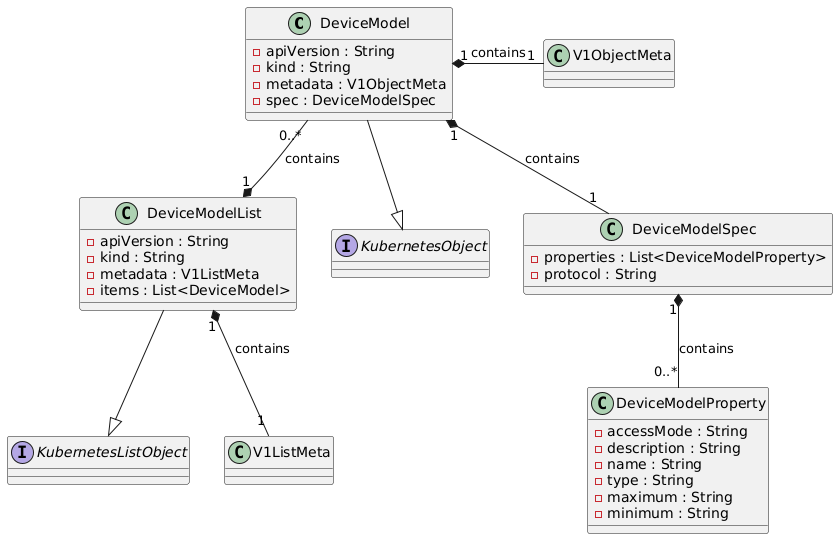
\includegraphics[width=0.95\linewidth]{pics/4-9devicemodel类图.png}
  \caption{DeviceModel 领域层的类图}
  \label{fig:4-9devicemodel}
\end{figure}

图 \ref{fig:4-9devicemodel} 展示了 DeviceModel 领域层的类图。在 KubeEdge 的 Device CRDs 中,DeviceModel 是用于描述设备模型的核心抽象,其设计旨在定义设备的静态属性和协议规范。具体而言,DeviceModel 包含以下关键属性:协议(Protocol)描述设备支持的通信协议及其相关参数;设备模型属性(DeviceModelProperty)表示设备的具体特性,包括属性类型、取值范围以及默认值;属性元数据(Metadata)提供关于设备属性的额外信息,例如访问权限以及更新频率等。

\begin{figure}[ht]
  \centering
  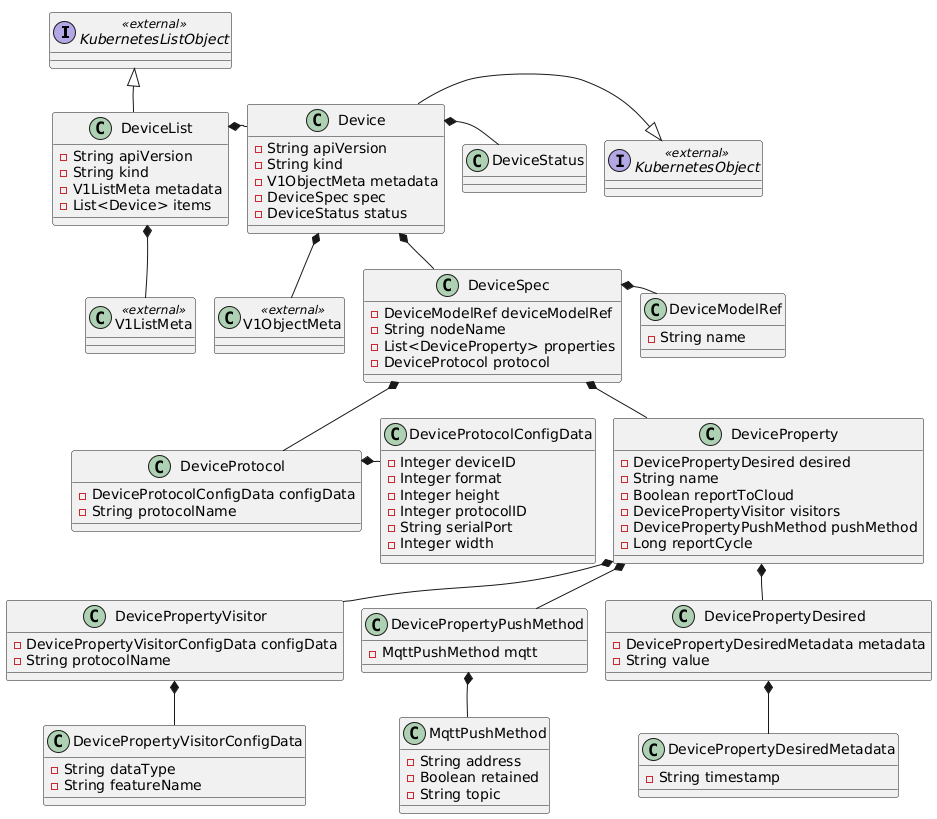
\includegraphics[width=\linewidth]{pics/4-8device类图.png}
  \caption{Device 领域层的类图}
  \label{fig:4-8device}
\end{figure}

图 \ref{fig:4-8device} 展示了 Device 领域层的类图,Device 是用于描述具体设备实例的核心抽象,其设计旨在将物理设备与对应的设备模型关联起来,从而实现从抽象到具体的映射。Device 的核心定义可以分为以下几个部分:设备规格(Spec)通过 deviceModelRef 关联设备元模型,继承设备模型中定义的静态属性和协议规范,同时允许在实例级别通过 properties 属性覆盖设备模型中的默认配置,以满足具体设备的个性化需求;通信协议配置(Protocol)进一步细化了物理设备的通信参数,确保设备与云边协同系统的无缝对接;设备状态(Status)模块则实现了数字孪生体的状态同步,实时记录设备的运行数据与健康状态,为上层应用提供可靠的监控能力。此外,扩展功能模块集成了基于 MQTT 的数据推送策略,通过 reportCycle 字段控制设备数据的上报频率,从而优化网络资源的使用效率。这一设计不仅有效实现了 DeviceModel 中定义的抽象模型,还为实际物理设备的接入与管理提供了灵活且高效的解决方案。

\begin{figure}[ht]
  \centering
  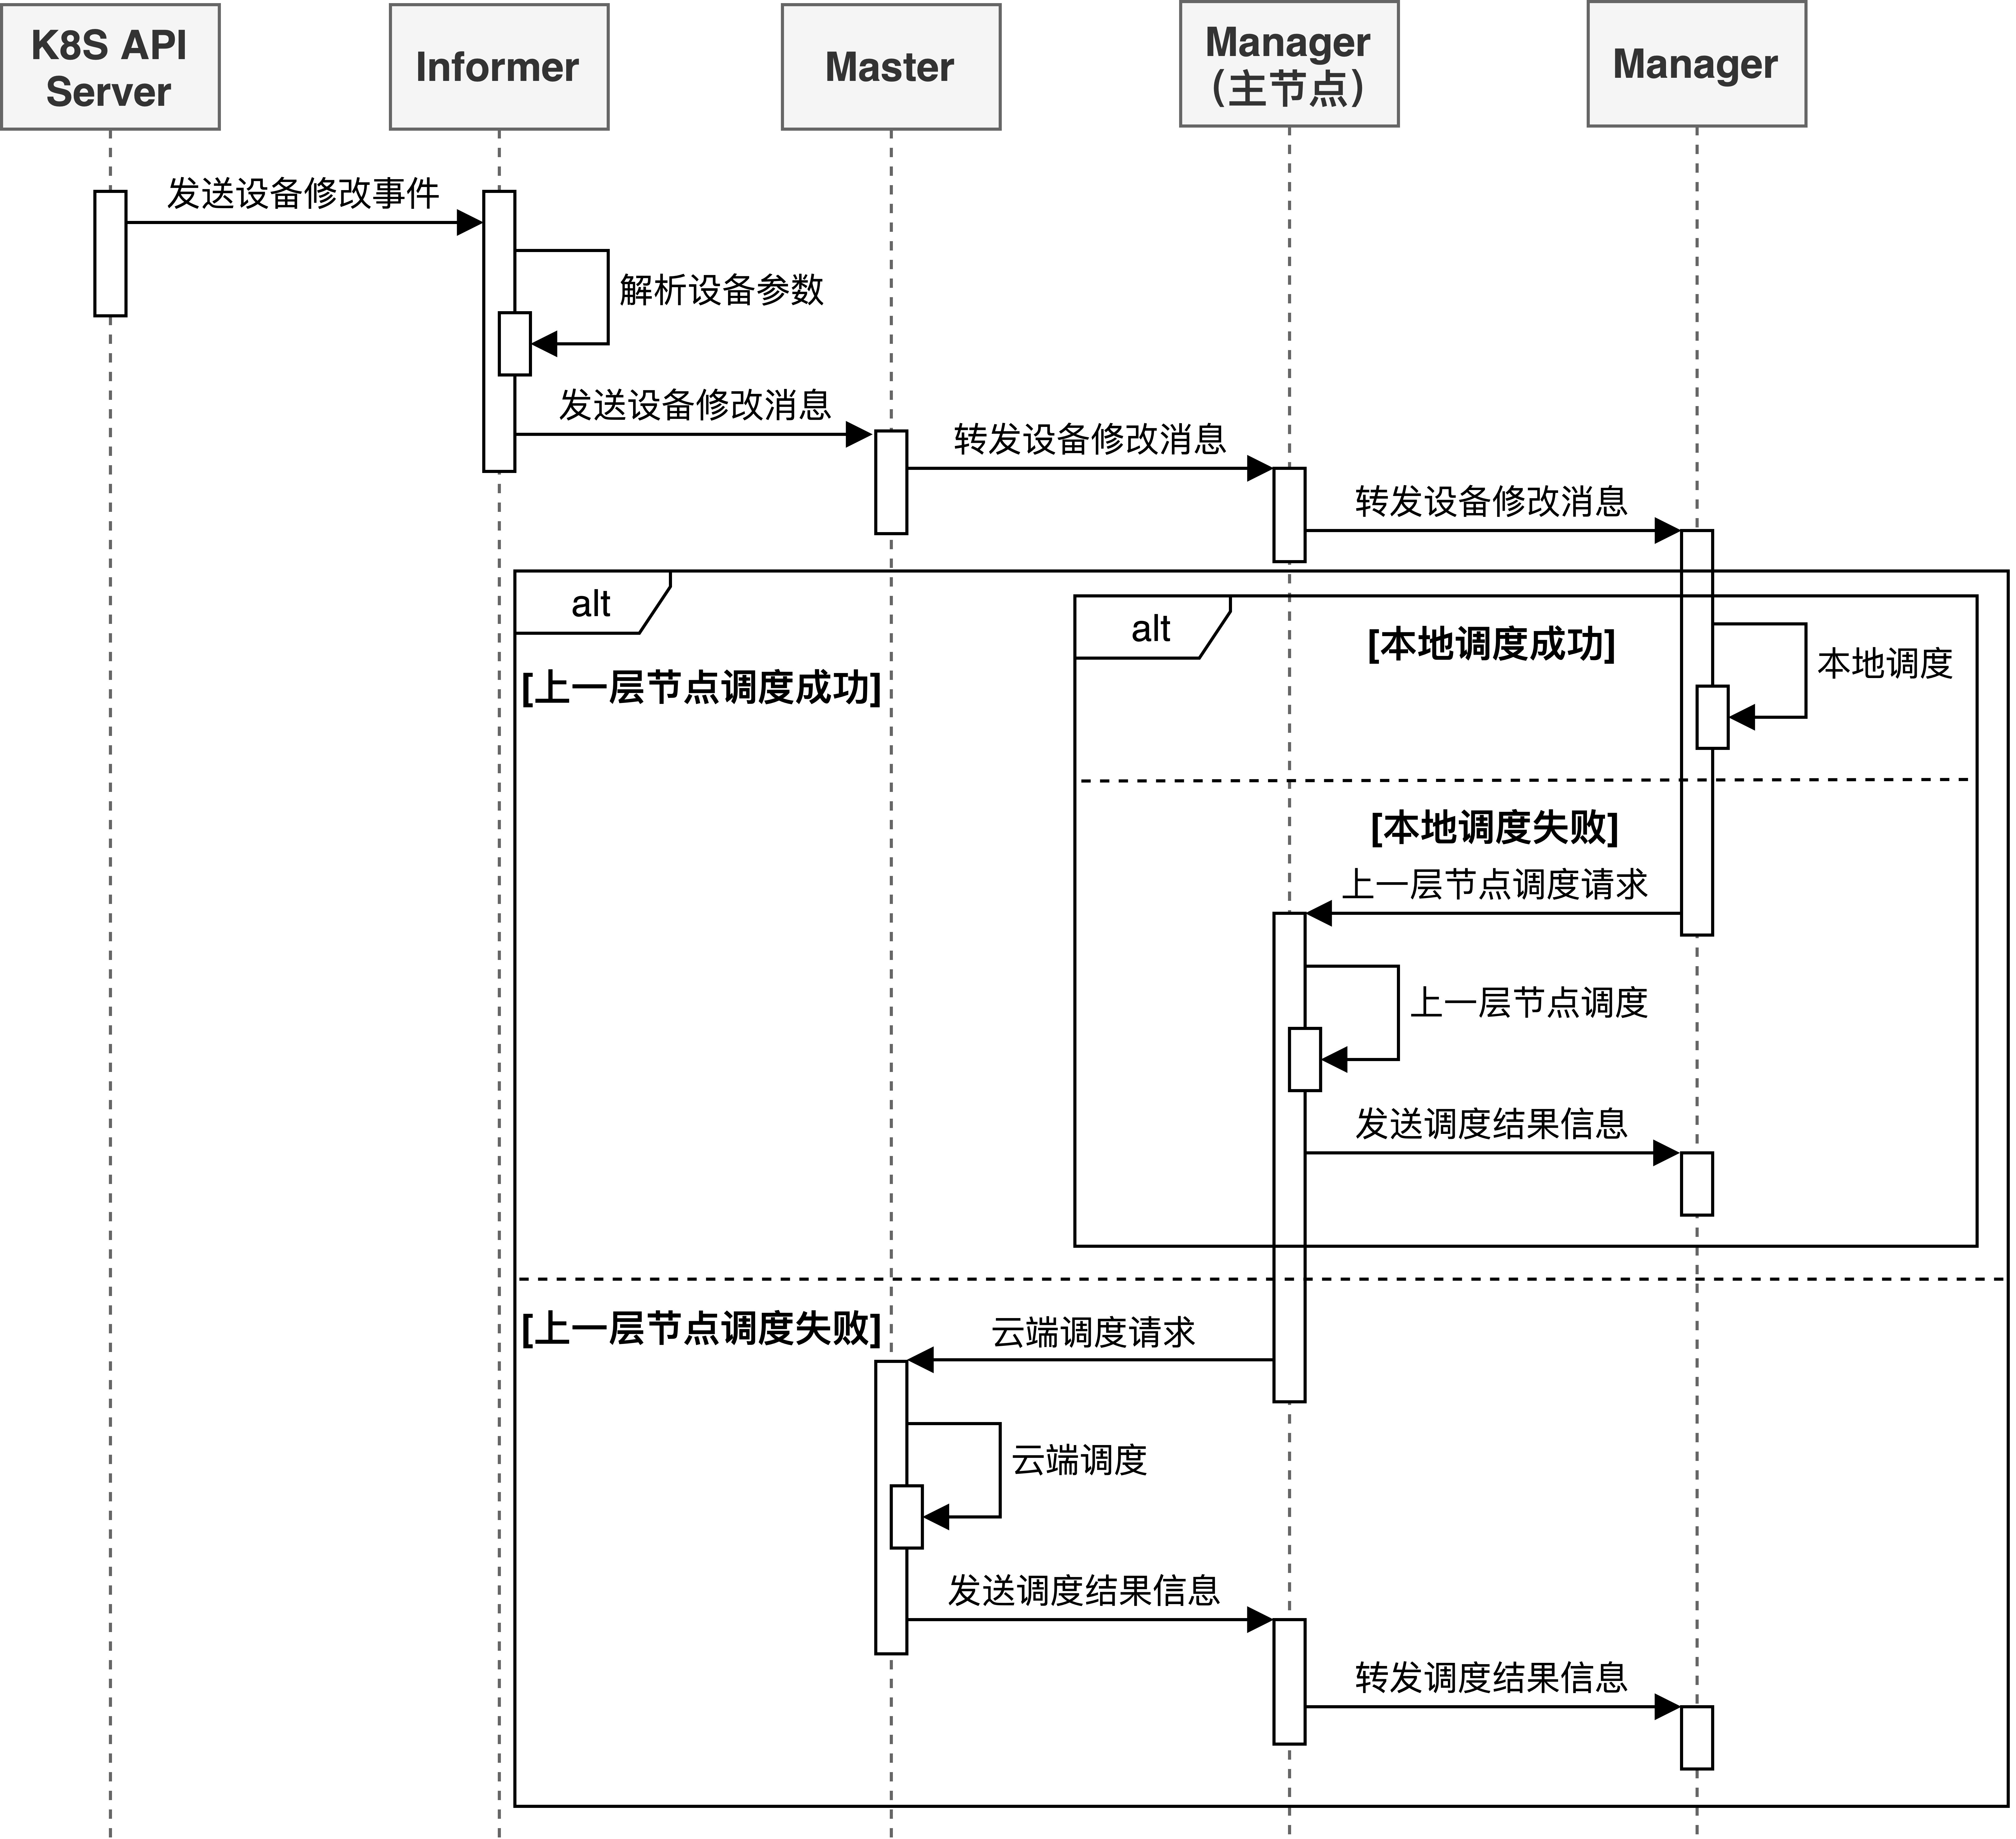
\includegraphics[width=\linewidth]{pics/4-10informer时序.png}
  \caption{基于 Informer 的设备状态监听与调度流程的时序图}
  \label{fig:4-10informer}
\end{figure}

在上述设计的基础上,本文通过 Kubernetes 的 ListAndWatch 方法实现了对设备状态的动态监听。如图\ref{fig:4-10informer}所示,Informer 组件会通过 API Server 提供的长连接机制,实时接收设备信息的变更事件。当设备信息发生变更时,API Server 会主动向客户端推送修改事件,Informer 组件则根据设备的静态信息提取出单次数据采集量和采集频率等关键的变更,并将这些信息封装为 Akka 消息(Message)发送至云端调度器 Master。Master 接收到消息后,将其转发至边缘树状集群主节点 Manager,再由 Manager 将消息分发至设备直连节点的边端管理器,从而触发云边协同环境下的多层次调度机制。设备直连节点的边端管理器会根据设备的变更情况尝试进行本地调度。若本地资源无法满足设备流式数据的需求,则将无法处理的请求转发至上一层节点的边端管理器,触发上一层调度。如果边缘树状集群的资源仍然不足,则进一步将请求转发至云端管理器 Master,由云端完成全局调度。这一多层次的调度机制不仅充分利用了边缘计算的本地化优势,还通过云端的全局视角确保了系统的整体性能与可靠性。

\subsubsection{资源动态部署机制}
\label{sec:deploy-resource}

为满足云边协同系统运行时部署AI模型推理实例等核心负载的需求,本文设计了基于Kubernetes原生资源的资源动态部署机制。该机制通过预置标准化的部署模板,实现了对负载实例的自动化部署。

\begin{figure}[ht]
  \centering
  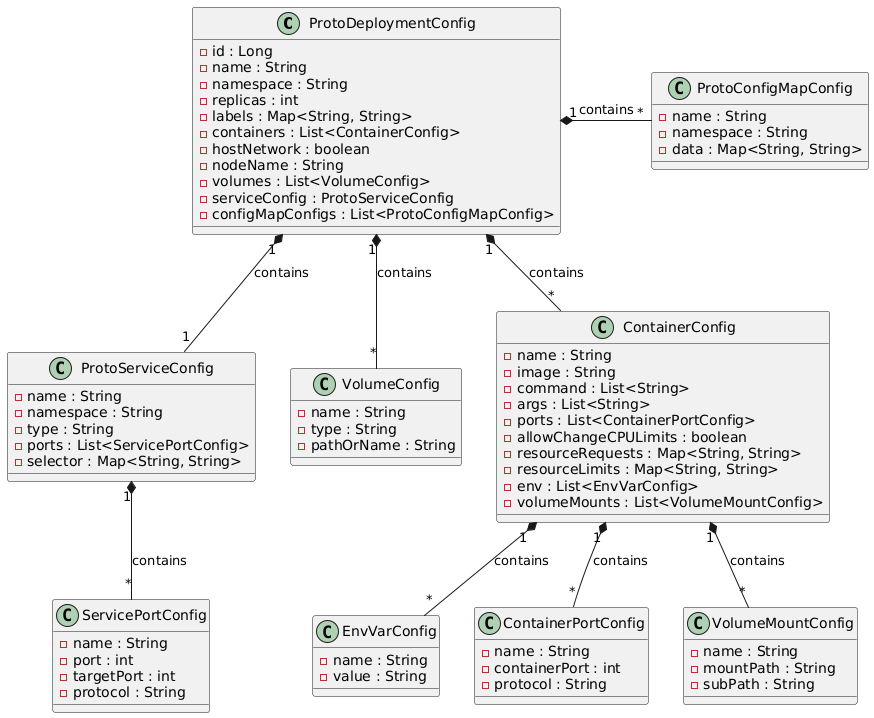
\includegraphics[width=\linewidth]{pics/4-11proto.png}
  \caption{资源动态部署机制的领域层类图}
  \label{fig:4-11proto}
\end{figure}

图 \ref{fig:4-11proto} 展示了资源动态部署机制的领域层类图,核心组件ProtoDeploymentConfig作为配置模板的核心载体,通过组合ProtoServiceConfig和ProtoConfigMapConfig,构建了完整的负载部署配置拓扑。具体而言,ProtoDeploymentConfig以对象图形式封装了Kubernetes Deployment的全部配置参数,包括容器镜像、资源配额、存储卷挂载等运行时属性,并通过ContainerConfig实现对容器启动参数的细粒度控制。当系统调用Kubernetes API时,该配置对象会自动转化为Deployment资源的创建请求,通过API Server完成Pod实例的编排。同时,嵌套的ProtoServiceConfig将通过标签选择器(selector)与Deployment形成语义绑定,确保服务发现机制能够精准路由流量至对应的Pod实例;而ProtoConfigMapConfig则将配置数据以键值对形式注入到Pod中,实现了配置参数的动态更新能力。此外,本设计通过hostNetwork、nodeName等属性实现了对节点亲和性调度的显式控制,并支持HostPath、PersistentVolume等多类型存储卷的挂载配置,使得系统能够灵活适配云边环境中的异构资源约束。这一核心负载原型设计通过领域对象到 Kubernetes 资源的自动化映射机制,将复杂的配置过程封装为标准化接口,使开发人员能够专注于深度学习模型的设计与开发,而无需关心底层部署细节,从而显著降低了云边协同系统的集成复杂度。

\subsection{模型推理服务}

本文的AI模型推理服务专注于推理部署环节。用户需将训练完成的AI模型(包含模型结构与权重)预先上传至对象存储服务,支持MinIO或阿里云等第三方存储方案。本文采用MinIO作为默认存储后端,并通过RESTful API实现模型文件的上传和下载。

\subsubsection{模型推理实例镜像打包}

在工业化的 AI 模型推理领域,现有的成熟框架(如 TensorFlow Serving 和 TorchServe)已经能够通过配置文件挂载预训练模型,实现高效部署推理服务。然而,在云边协同环境中,由于计算节点的异构性问题,这些框架在实际应用中面临诸多挑战。例如,计算节点可能基于不同的硬件架构(如 AMD64、ARMv7 或 ARMv8),并且即使在同一架构下(如 AMD64),也可能存在指令集加速支持的差异(如 AVX2)。为了屏蔽底层硬件差异并减少重复工作,本文为不同架构打包了适配的镜像,如表\ref{tab:multi-arch-images} 所示。具体而言,本文利用 QEMU 模拟多种硬件架构,并结合 Bazel 工具链编译了适配不同架构的 TensorFlow 和 TensorFlow Serving。随后,将编译结果封装为多架构 Docker 镜像,以满足云边协同环境中的多样化需求。在模型部署阶段,系统通过 Kubernetes 的节点标签(Node Labels)机制,根据节点的硬件架构信息动态选择与之匹配的镜像版本,从而确保镜像与目标节点的兼容性。

\begin{table}[ht]
    \renewcommand{\arraystretch}{1.5}
    \centering
    \caption{不同架构的 TensorFlow Serving 镜像}
    \label{tab:multi-arch-images}
    \begin{tabular}{lll}
        \toprule
        \textbf{架构类型} & \textbf{镜像名称} & \textbf{特性说明} \\
        \midrule
        ARM32 (32-bit) & tensorflow-serving:latest-arm32 & 无SIMD加速 \\
        ARM64 (64-bit) & tensorflow-serving:latest-arm64 & NEON指令集优化 \\
        AMD64 & tensorflow-serving:latest-amd64 & 默认支持AVX2加速 \\
        AMD64 (no-AVX2) & tensorflow-serving:noavx2-amd64 & 不依赖AVX2指令集 \\
        \bottomrule
    \end{tabular}
\end{table}

\subsubsection{模型推理实例转换}

尽管 TensorFlow Serving 提供了高效的推理能力,但不同框架训练的模型可能存在兼容性问题。例如,使用 PyTorch 或 Keras 训练的模型无法直接部署到 TensorFlow Serving 中。为此,本文设计了一个微服务模块,用于自动化完成模型的转换与封装。该模块通过解析原始模型文件,将其转换为 ONNX 格式,并生成适配目标推理框架的配置文件,从而简化了跨框架部署的复杂性。该模块的生命周期如图\ref{fig:4-12trans}所示,主要包括创建状态、下载状态、模型转换状态、上传模型状态、失败状态和结束状态,各状态间的转换遵循严格的工作流控制机制,具体如下:

\begin{figure}[ht]
  \centering
  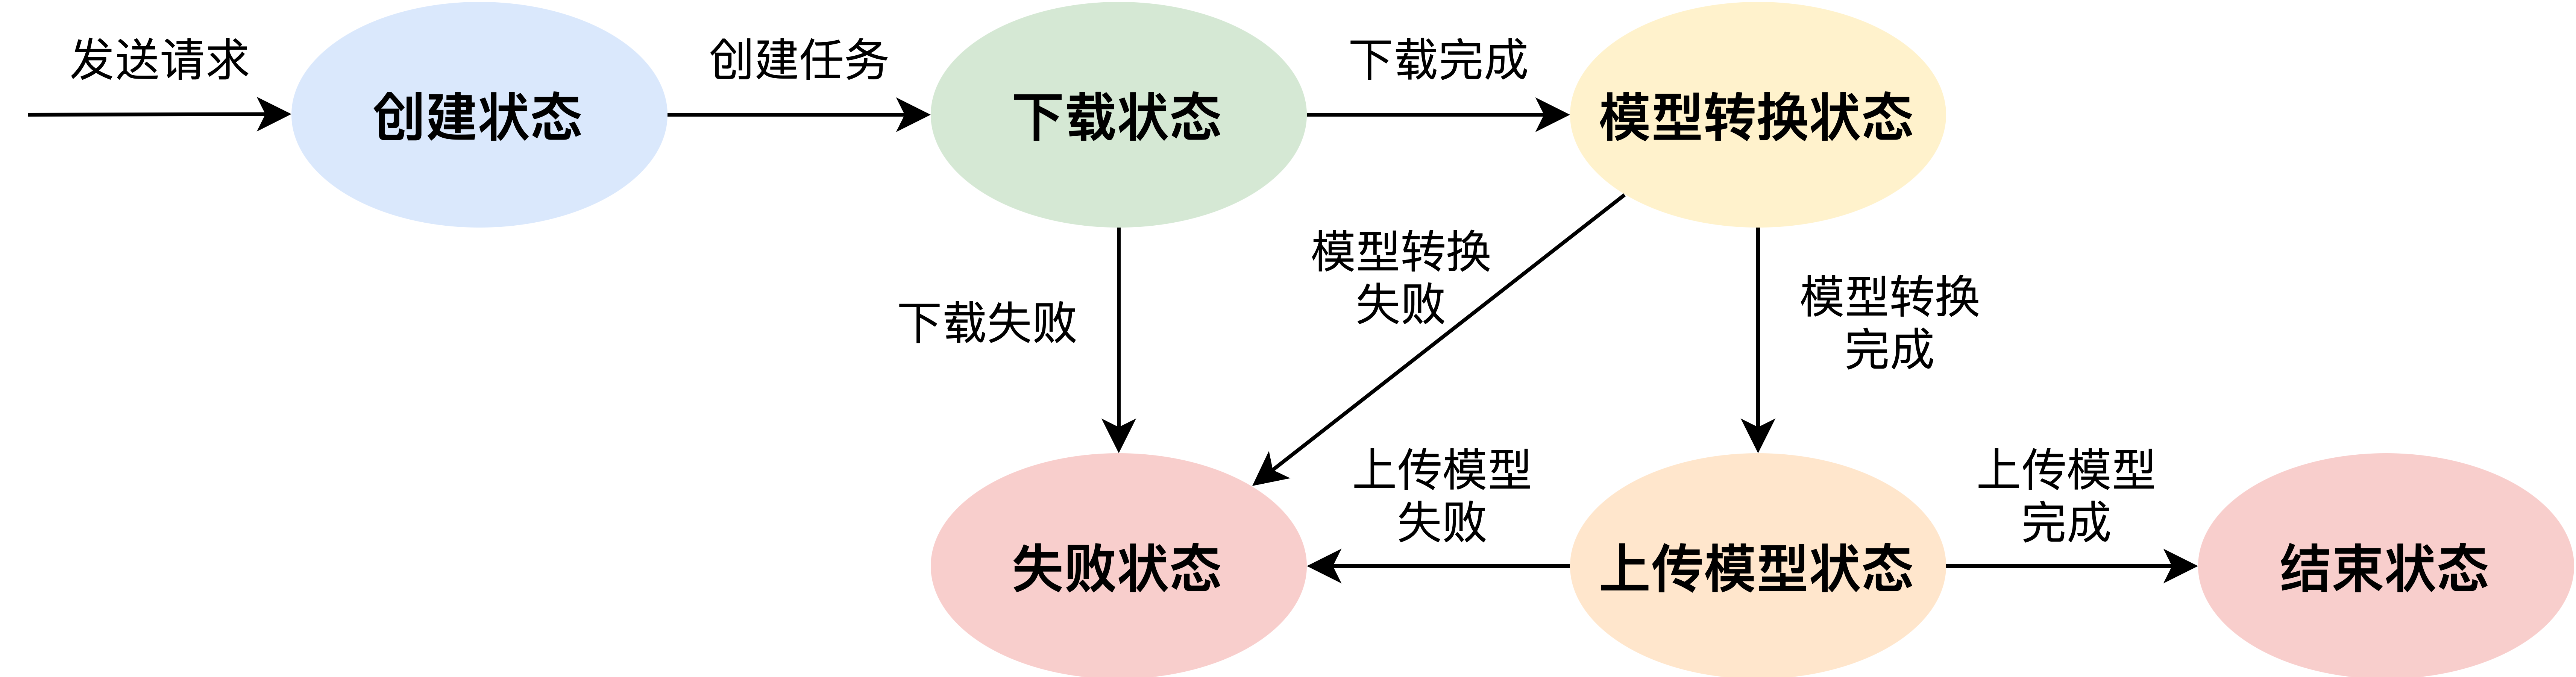
\includegraphics[width=\linewidth]{pics/4-12模型转换.png}
  \caption{AI模型转换模块的生命周期}
  \label{fig:4-12trans}
\end{figure}

\begin{itemize}
    \item \textbf{创建状态:} 系统接收转换请求后,首先验证输入参数的有效性,包括源模型路径、目标格式兼容性以及 MinIO 存储连接状态。验证通过后,系统生成唯一任务标识符并创建任务记录,并客户端返回任务 ID,同时启动异步模型转换流程。
    \item \textbf{下载状态:} 进入异步下载处理后,系统首先在临时存储中建立隔离的工作目录结构,然后从 MinIO 对象存储获取源模型。此阶段支持多种模型存储形式,包括单文件模型、目录结构模型(如 TensorFlow SavedModel)以及压缩包模型。若源模型为压缩格式,系统会自动解压并识别其中的有效模型文件。下载过程中如遇网络故障或权限问题,任务将直接转入失败状态。
    \item \textbf{模型转换状态:} 模型下载完成后,系统根据源格式和目标格式确定转换路径。首先将源模型转换为 ONNX 中间表示,再从 ONNX 转换为目标格式。转换过程保留计算图结构、权重参数和输入输出规格,同时执行模型验证以确保转换精度达到预期要求。
    \item \textbf{上传模型状态:} 模型成功转换后,系统将结果模型打包并上传至用户指定的 MinIO 存储位置。此阶段会自动处理不同模型格式的特殊要求,例如将目录结构模型压缩为 ZIP 文件,或者将大型模型分片上传以提高传输可靠性。
    \item \textbf{失败和结束状态:} 整个生命周期中的任何阶段出现异常,均会触发失败状态转换。对于不同类型的失败,系统应用了差异化的恢复策略,例如网络故障会触发重试机制,而格式不兼容则直接标记为永久性失败。无论成功还是失败,系统最终都会清理临时资源,确保服务器资源得到有效释放。
\end{itemize}

\subsubsection{模型推理实例动态部署}

\begin{figure}[ht]
  \centering
  \includegraphics[width=\linewidth]{pics/4-13deployai.png}
  \caption{模型推理实例部署的时序图}
  \label{fig:4-13deployai}
\end{figure}

结合上述模型推理实例镜像打包、模型推理实例转换模块以及 \ref{sec:deploy-resource} 小节中描述的资源动态部署机制,可以实现模型推理实例动态部署流程。如图 \ref{fig:4-13deployai} 所示,当用户通过 HTTP 请求发起模型推理实例部署请求时,系统内置的控制器(Controller)会捕获该请求并将其转发至云端管理器(Master)。云端管理器在接收到请求后,会创建一个专门负责部署任务的 Actor(Deploy Actor),并将与部署相关的完整上下文信息传递给该 Actor,以驱动后续的部署流程。Deploy Actor 首先解析目标模型的框架类型。若检测到目标推理引擎与模型框架之间存在兼容性问题,则触发模型转换流程,调用模型转换模块完成格式适配。随后,Deploy Actor 会轮询确认模型转换的成功状态,并从 MinIO 存储中获取模型文件的存储地址。该地址通过边缘集群主节点被转发至目标部署节点,目标节点则从 MinIO 下载模型文件并完成解压等预处理操作。在此基础上,Deploy Actor 根据节点加入时由 Informer 提供的节点架构信息,结合资源动态部署机制生成适配目标节点资源环境的核心部署配置。最终,Deploy Actor 通过 Kubernetes API Server 创建相应的 Deployment 和 Service 等资源对象,从而完成整个部署流程。

\subsubsection{模型推理实例批处理测试}

当模型推理实例部署到节点后,若该模型支持批处理(batch processing),系统会触发批处理测试以评估模型在目标节点上的性能表现并确定最优的批处理规模(batch size)。如图\ref{fig:4-14batch}所示,批处理测试分为两个阶段:初始快速上升阶段和精细化搜索阶段。在快速上升阶段,系统以$2^n$次方指数增长的方式逐步增加批处理规模,直至出现资源过载(如内存溢出OOM、CPU/GPU使用率饱和等)为止。此时,系统确认查找范围并进入精细化搜索阶段,采用二分法逐步缩小批处理规模,直至找到系统可承受的最大批处理值。在此过程中,系统同时记录每个批处理规模下的平均数据处理时间,并以最小化单个数据的平均处理时间为优化目标。需要注意的是,虽然批处理通常能够显著降低单位数据的推理开销,但过大的批处理规模可能导致资源竞争加剧,反而降低整体性能。

\begin{algorithm}[ht]
\caption{批处理规模优化测试算法}
\label{alg:batch_size_optimization_simple}
\begin{algorithmic}[1]
\REQUIRE 模型 $Model$, 输入样例 $Input$, 初始批量 $B_{init}$
\ENSURE 最优批处理大小 $B_{opt}$, 最优单数据平均处理时间 $t_{avg\_opt}$

\STATE Initialize $B_{max} \leftarrow 0$, $t_{avg\_opt} \leftarrow \infty$, $B_{opt} \leftarrow 0$

\STATE $B \leftarrow B_{init}$
\WHILE{$B$ succeeds}
  \STATE $(t_{total}, t_{avg}) \leftarrow$ GetTime($B$)
  \STATE $B_{max} \leftarrow B$
  \IF{$t_{avg} < t_{avg\_opt}$}
    \STATE $t_{avg\_opt} \leftarrow t_{avg}$, $B_{opt} \leftarrow B$
  \ELSIF{$t_{avg} > t_{avg\_opt}$} 
    \STATE break \COMMENT{提前终止搜索,避免无效的更大批量}
  \ENDIF
  \STATE $B \leftarrow B \times 2$ \COMMENT{批处理大小加倍}
\ENDWHILE
\STATE $lower \leftarrow B_{max}$, $upper \leftarrow B$ \COMMENT{$B$是首次失败或性能变差的批量}
\WHILE{$lower < upper - 1$}
  \STATE $B_{mid} \leftarrow \lfloor(lower + upper) / 2\rfloor$
  \IF{$B_{mid}$ succeeds}
    \STATE $(t_{total}, t_{avg}) \leftarrow$ GetTime($B_{mid}$)
    \STATE $lower \leftarrow B_{mid}$
    \IF{$t_{avg} < t_{avg\_opt}$}
      \STATE $t_{avg\_opt} \leftarrow t_{avg}$, $B_{opt} \leftarrow B_{mid}$
    \ENDIF
  \ELSE
    \STATE $upper \leftarrow B_{mid}$
  \ENDIF
\ENDWHILE

\RETURN $B_{opt}$, $t_{avg\_opt}$
\end{algorithmic}
\end{algorithm}

具体的算法如算法\ref{alg:batch_size_optimization_simple}所示。该算法的时间复杂度主要由两部分组成:第一阶段的指数增长搜索复杂度为 $O(\log B_{max})$,其中 $B_{max}$ 是系统能承受的最大批量;第二阶段的二分查找复杂度为 $O(\log(B - B_{max}))$,因此总复杂度为 $O(\log B_{max} + \log(B - B_{max}))$,整体表现为高效的对数级复杂度。在完成批处理规模优化测试后,系统会根据算法\ref{alg:batch_size_optimization_simple}确定的最优批处理大小 $B_{opt}$ 配置 TensorFlow Serving 的批处理参数。

\begin{figure}[ht]
  \centering
  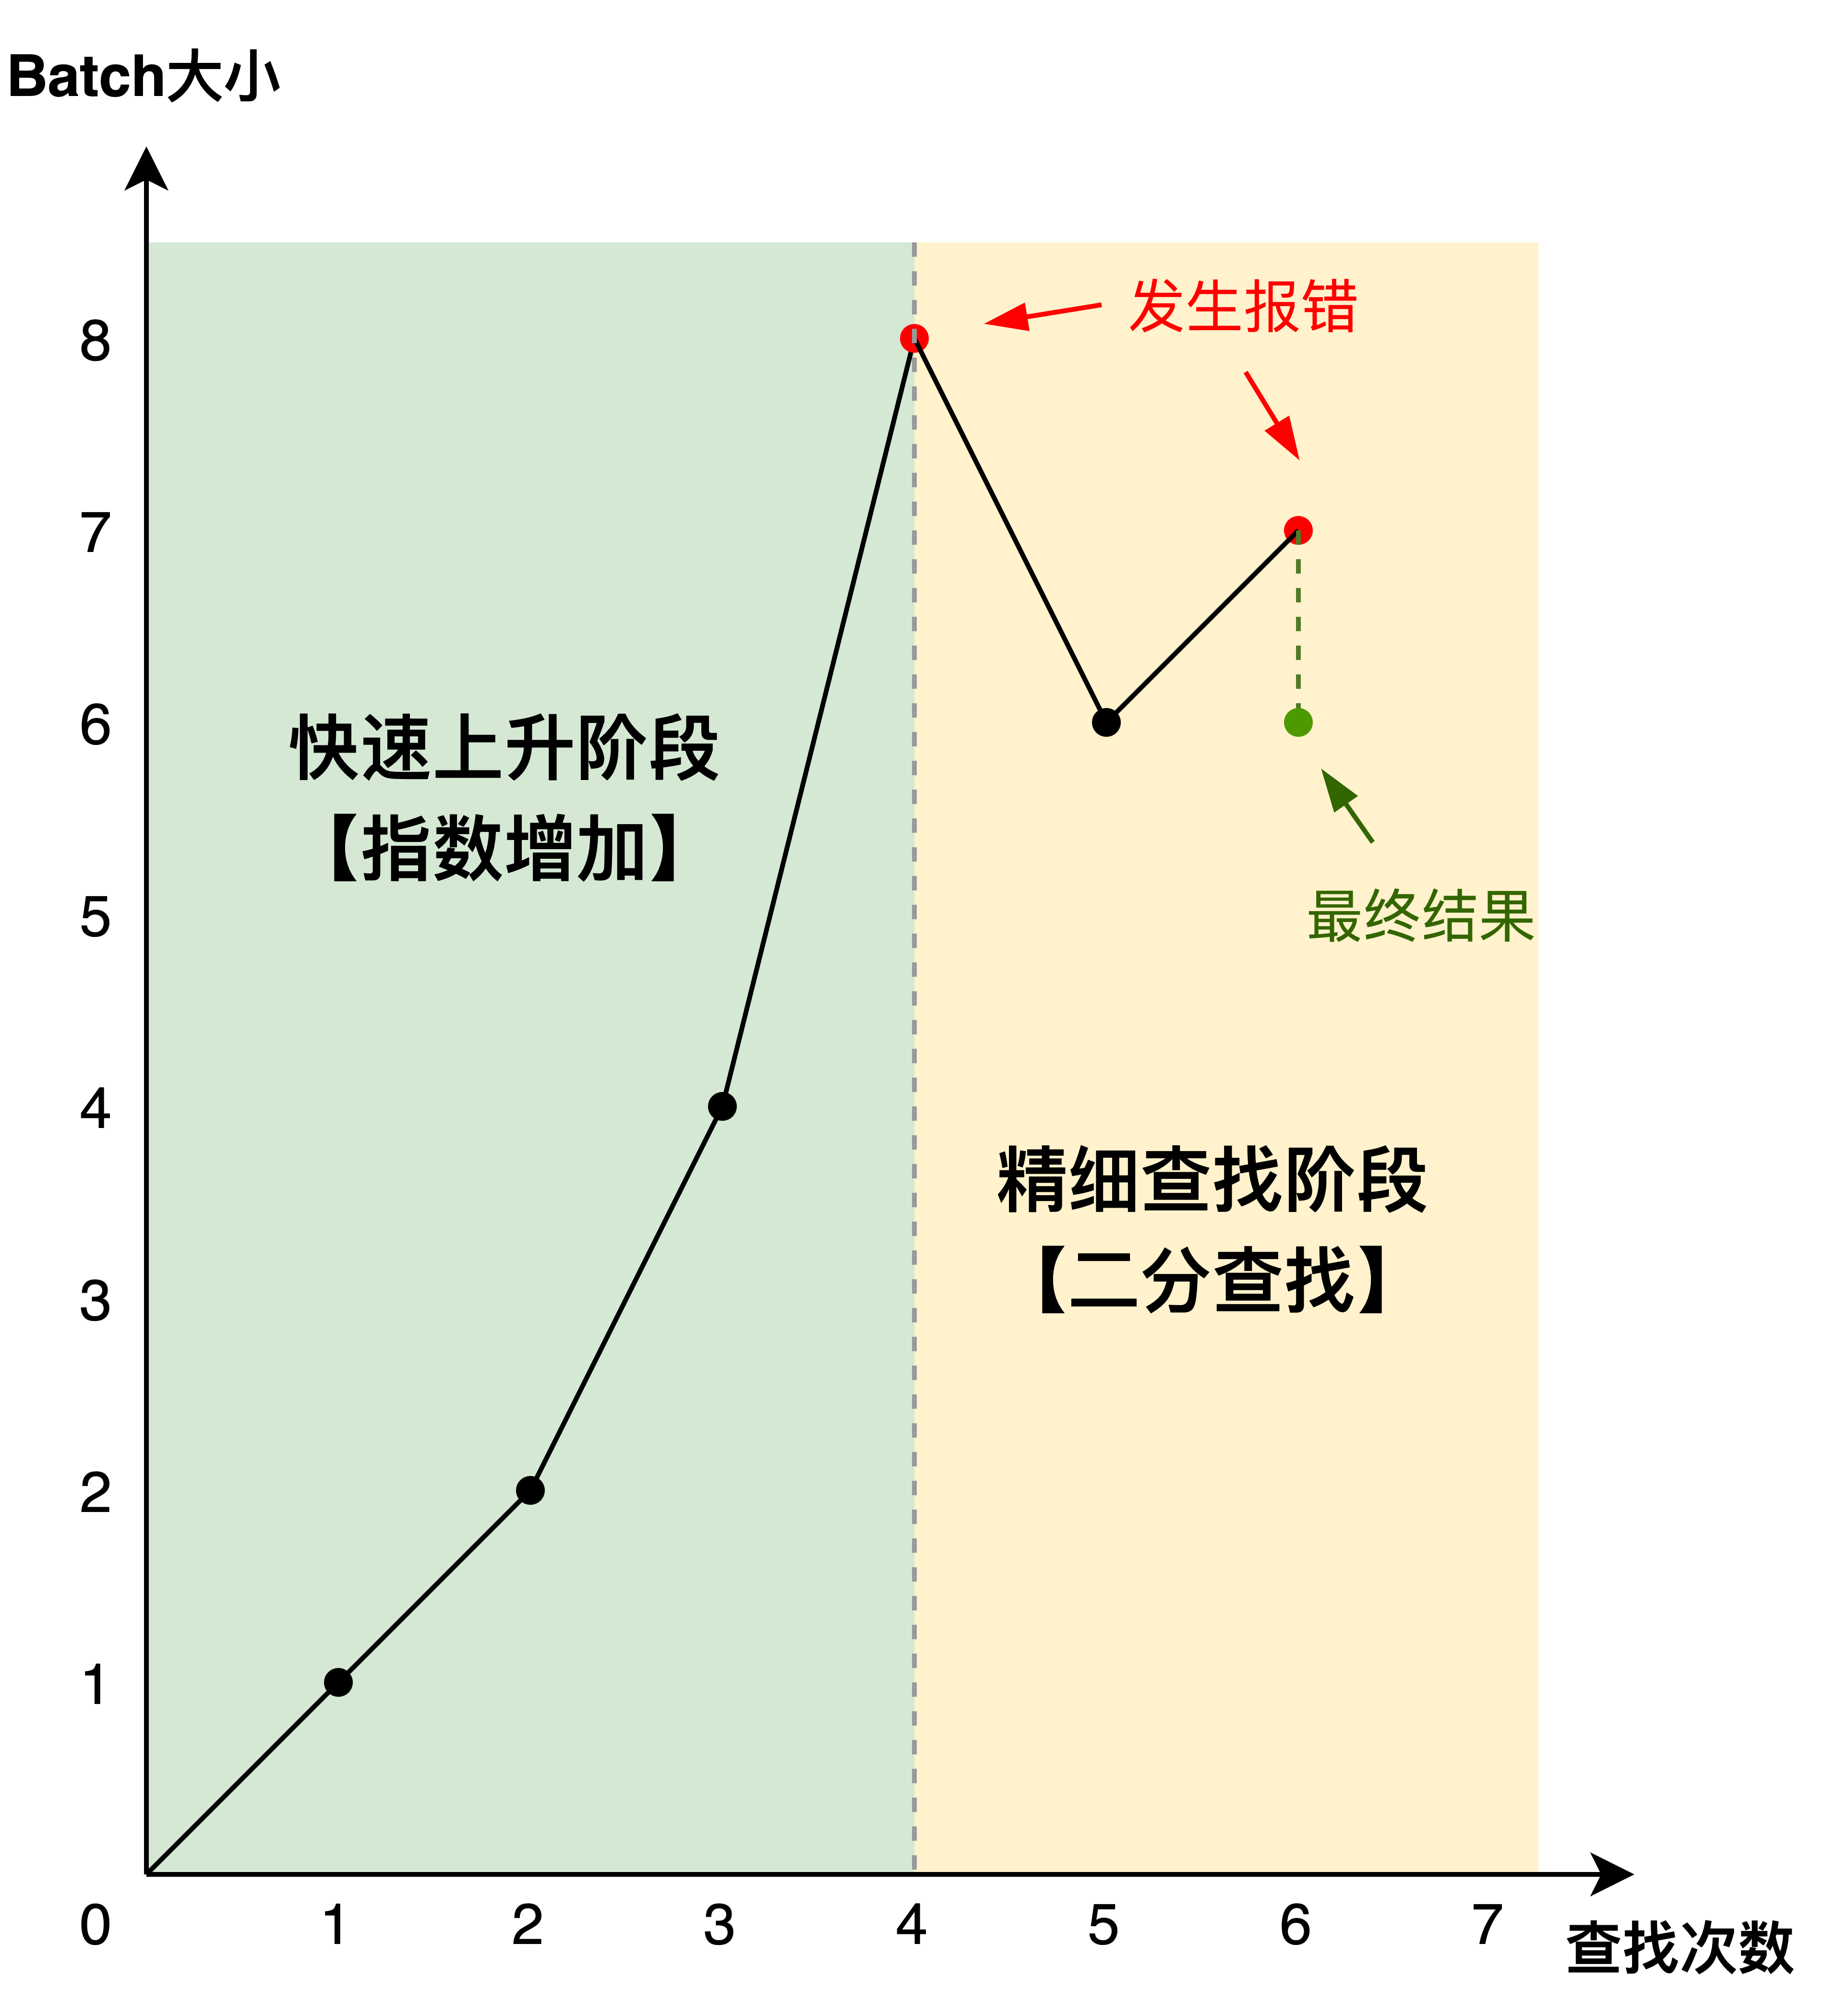
\includegraphics[width=0.6\linewidth]{pics/4-14批查找过程.png}
  \caption{模型推理实例批处理规模优化}
  \label{fig:4-14batch}
\end{figure}

\subsection{数据路由服务}

数据路由服务是KEAS系统中实现高效数据分发与处理的核心组件。该服务通过多个子 Actor 的协同工作完成复杂的任务调度与数据流转。这些子 Actor 由边缘管理器(Manager)动态创建和管理,主要负责订阅设备的流式数据、执行数据转发,并与本地模型推理服务模块进行交互。

\begin{figure}[ht]
  \centering
  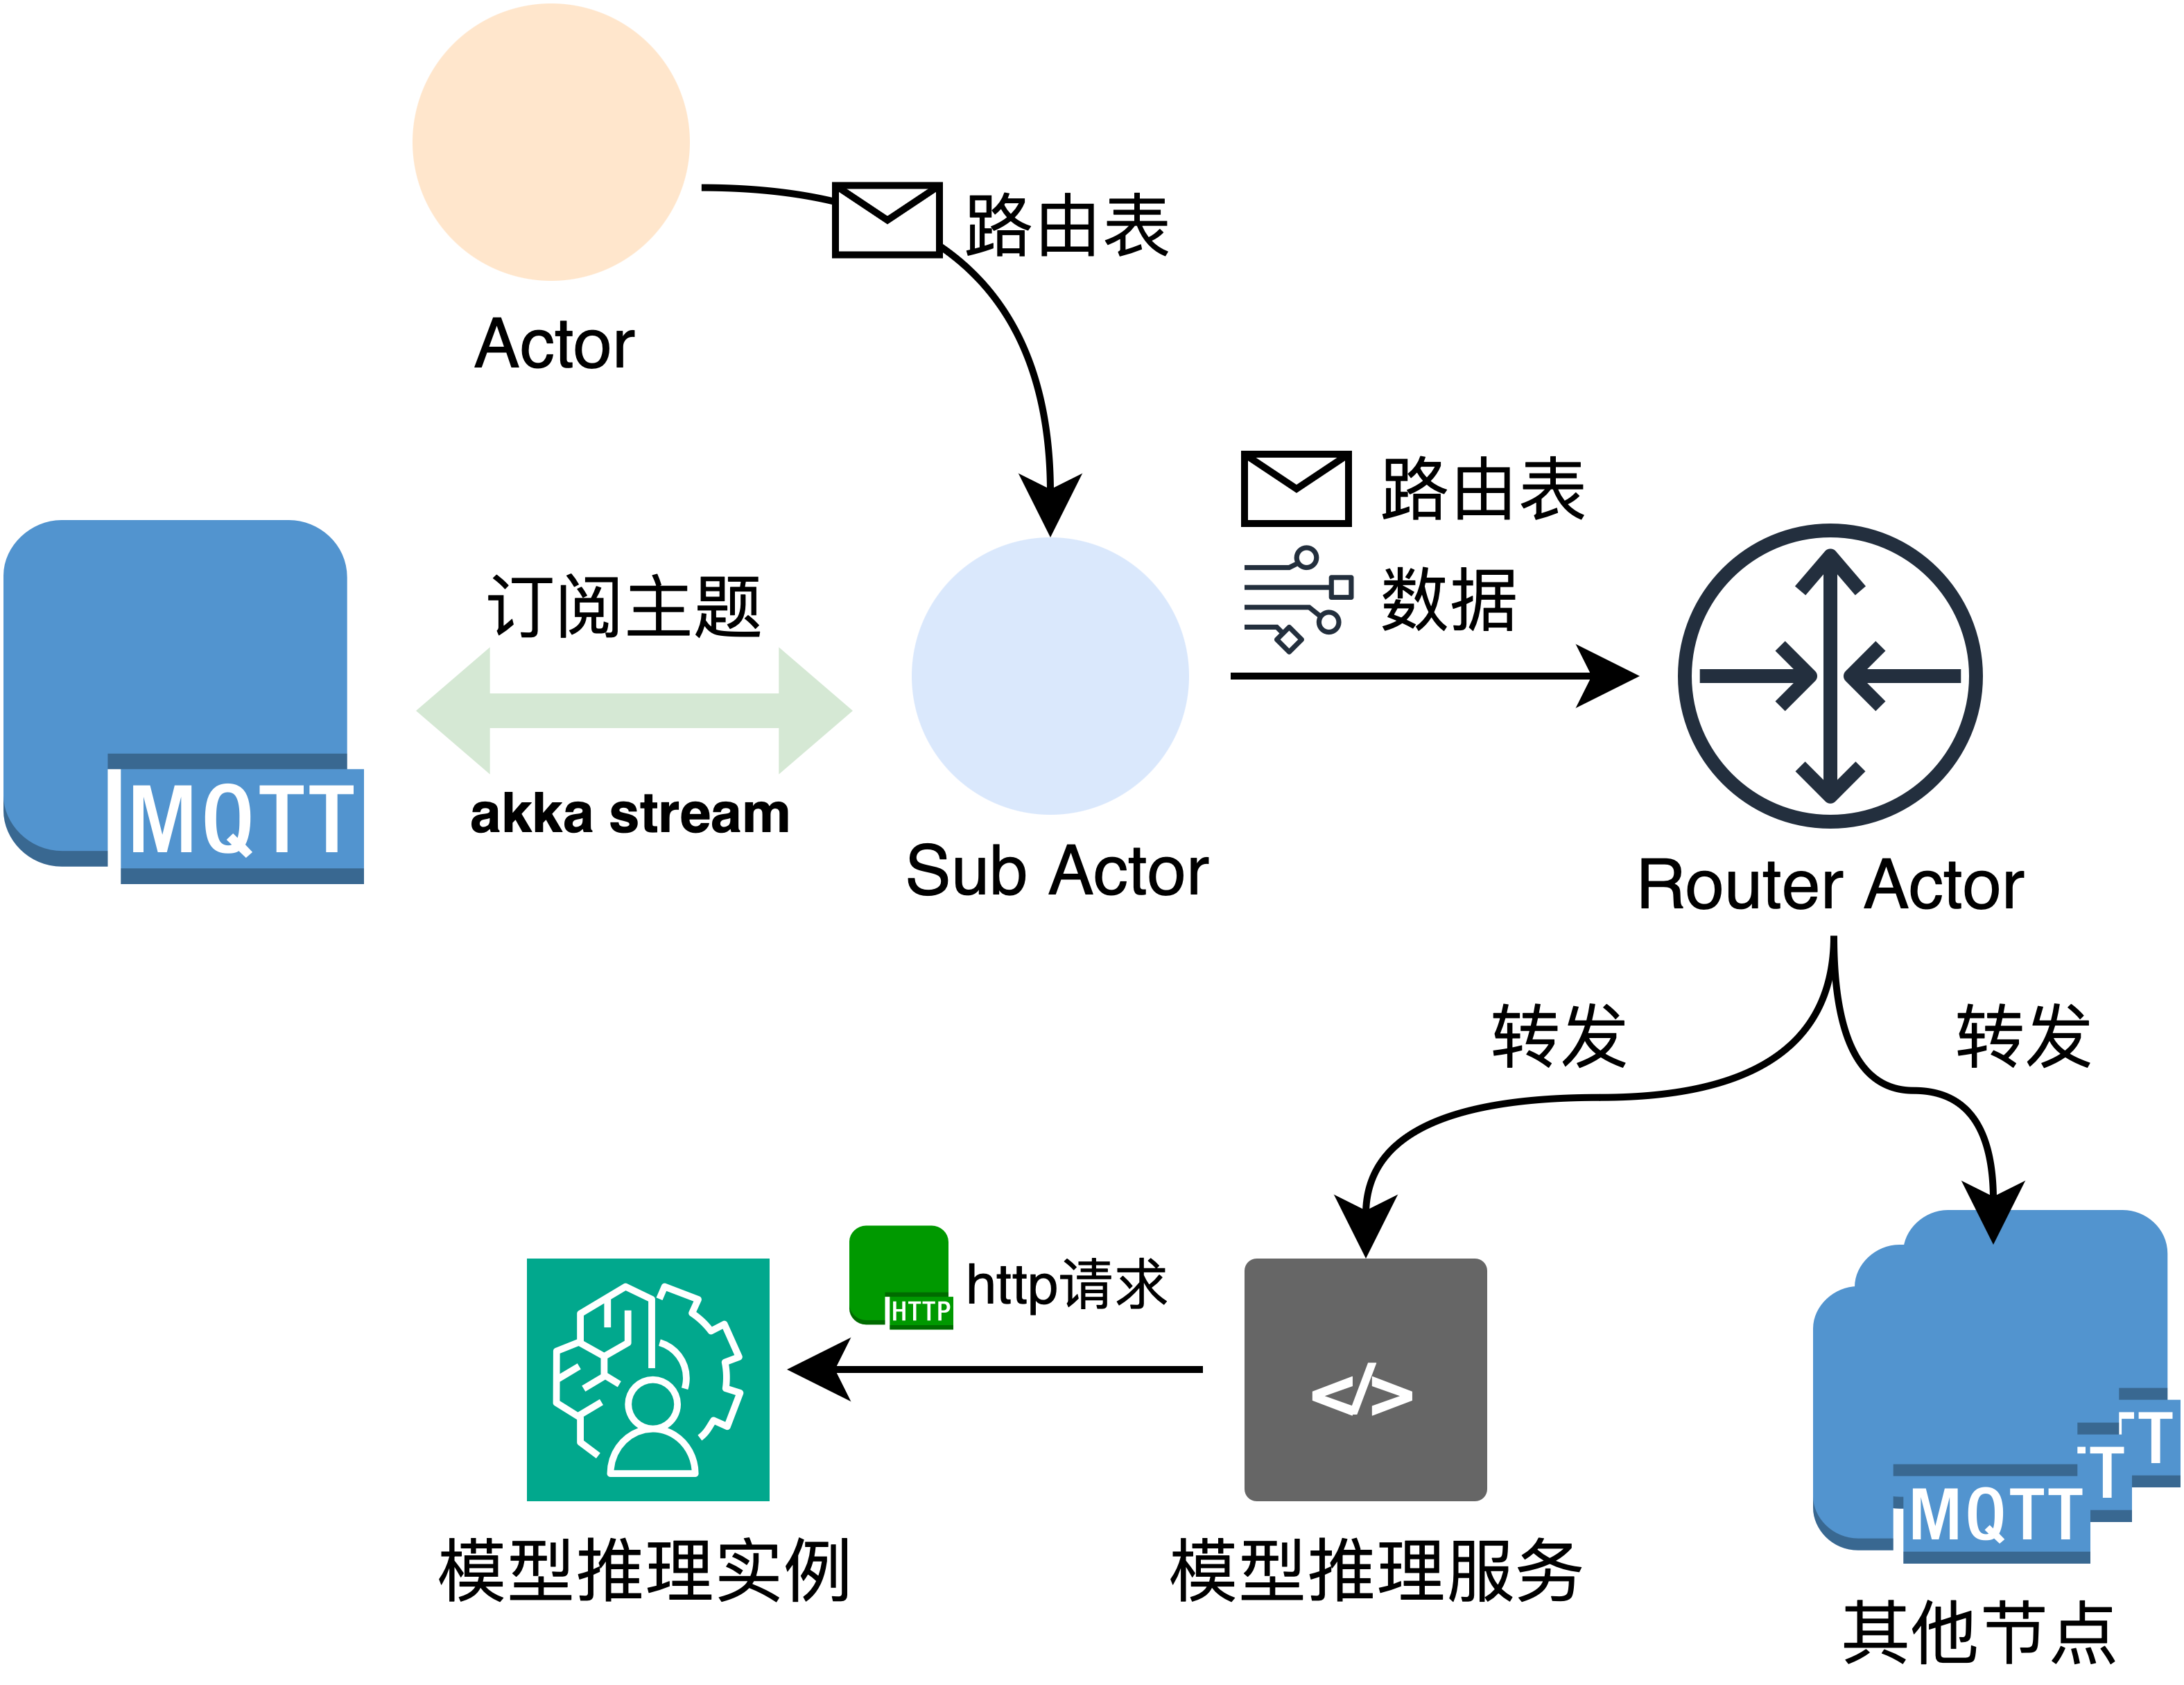
\includegraphics[width=0.75\linewidth]{pics/4-6worker.png}
  \caption{数据流路由服务架构}
  \label{fig:data-routing-architecture}
\end{figure}

如图\ref{fig:data-routing-architecture}所示,边缘管理器(Manager)根据云端管理器(Master)下发的全局路由表、或边缘集群生成的集群内部路由表,或本地生成的本地路由表,初始化一条包含订阅 Actor(Sub Actor)和路由 Actor(Router Actor)等核心组件的执行链。在数据采集阶段,Sub Actor 借助 Akka Streams 工具包连接 MQTT 消息代理(如 Mosquitto),以订阅来自设备的实时流式数据。随后,在数据分发阶段,Sub Actor 将接收到的数据及其对应的路由信息转发至 Router Actor。Router Actor 根据路由规则对数据流向进行决策:对于需要跨节点协作的数据,将其转发至其他节点的消息代理;对于需要本地处理的数据,则将其传递给本地的模型推理模块。最后,在数据处理阶段,模型推理服务模块对接收到的数据进行预处理,并将其整理为适合批处理的形式。经过预处理的数据通过 HTTP 或 gRPC 协议发送至模型推理实例,从而完成推理任务。此外,Router Actor 会持续监控模型推理服务模块的运行速度,并定期将相关性能指标上报给本地的边缘管理器,以实现运行状态的实时监控。这些监控数据首先被用于本地优化;随后,这些数据会被上传至上一层节点,为上一层节点的资源调度和负载均衡提供依据;同时,边缘树状集群主节点会进一步汇总这些数据并上传至云端,从而支持全局范围内的资源调度、性能分析以及长期趋势预测。

\subsection{系统监控服务}

系统监控服务不仅涵盖上一小节提到的对模型推理服务模块运行速度和任务队列状态的监控,还包括对云边环境下网络状况的全面监测,以确保调度决策的高效性与准确性。最终,所有监控数据将被汇总至 Prometheus,并通过 Grafana 进行可视化展示。

\subsubsection{网络监控探针}

本文采用主被动结合的混合监测方案,构建多维度网络性能评估体系。主动监测模块通过模拟网络流量直接测量关键性能指标,被动监测模块基于实际业务流量分析间接推断网络状态,二者共同覆盖端到端时延、带宽利用率、丢包率等核心维度,为云边协同环境中的资源调度与优化提供全面数据支撑。

主动监测模块通过可控的测试流量直接测量节点间的网络性能指标,主要包括端到端时延和带宽利用率两个方面。端到端时延测量利用 Ping 工具实现,系统定时发送探测请求并根据往返时间(RTT)计算网络延迟。为减少噪声干扰并提高数据稳定性,本文采用指数加权移动平均算法对时延数据进行平滑处理,其公式定义为:
为减少噪声干扰并提高数据稳定性,本文采用指数加权移动平均算法对时延数据进行平滑处理,其公式定义为:
\[
S_t = \alpha X_t + (1-\alpha)S_{t-1},
\]
其中,$S_t$ 表示当前时刻的平滑值,$X_t$ 为原始观测值,$\alpha \in (0,1]$ 为平滑系数,用于控制历史数据与当前观测值的权重分配。带宽测量采用 iPerf3 工具实现,通过动态调整 TCP 窗口大小与数据包分片策略,分别获取单向与双向带宽指标。此外,探测周期根据边缘节点的实时负载智能调整:在空闲时段采用短周期以实现快速响应,在高负载时段切换至长周期,从而在保证测量精度的同时降低系统开销,确保资源占用与性能需求之间的平衡。

被动监测模块基于实际业务流量的行为特征,通过分析节点间的通信数据间接推断网络性能。Node Exporter 是实现被动监测的核心工具,能够实时采集节点网卡的流量统计信息,包括接收/发送字节数、丢包率、错误率等关键指标。通过对单位时间内流量变化的分析,可以估算节点间的实际带宽利用率,并捕捉网络链路的拥塞状态。此外,基于 Node Exporter 采集的流量数据,结合历史记录和统计模型,可以间接估算节点间的网络时延。例如,通过分析数据包到达时间间隔及其分布特征,可以推断出网络延迟的大致范围。尽管被动监测方法的精度略低于主动测量,但其无需额外的探测流量,适合在高负载或受限环境中使用,从而为系统的整体性能评估提供了补充视角。

\subsubsection{监控汇总模块}

\begin{figure}[ht]
  \centering
  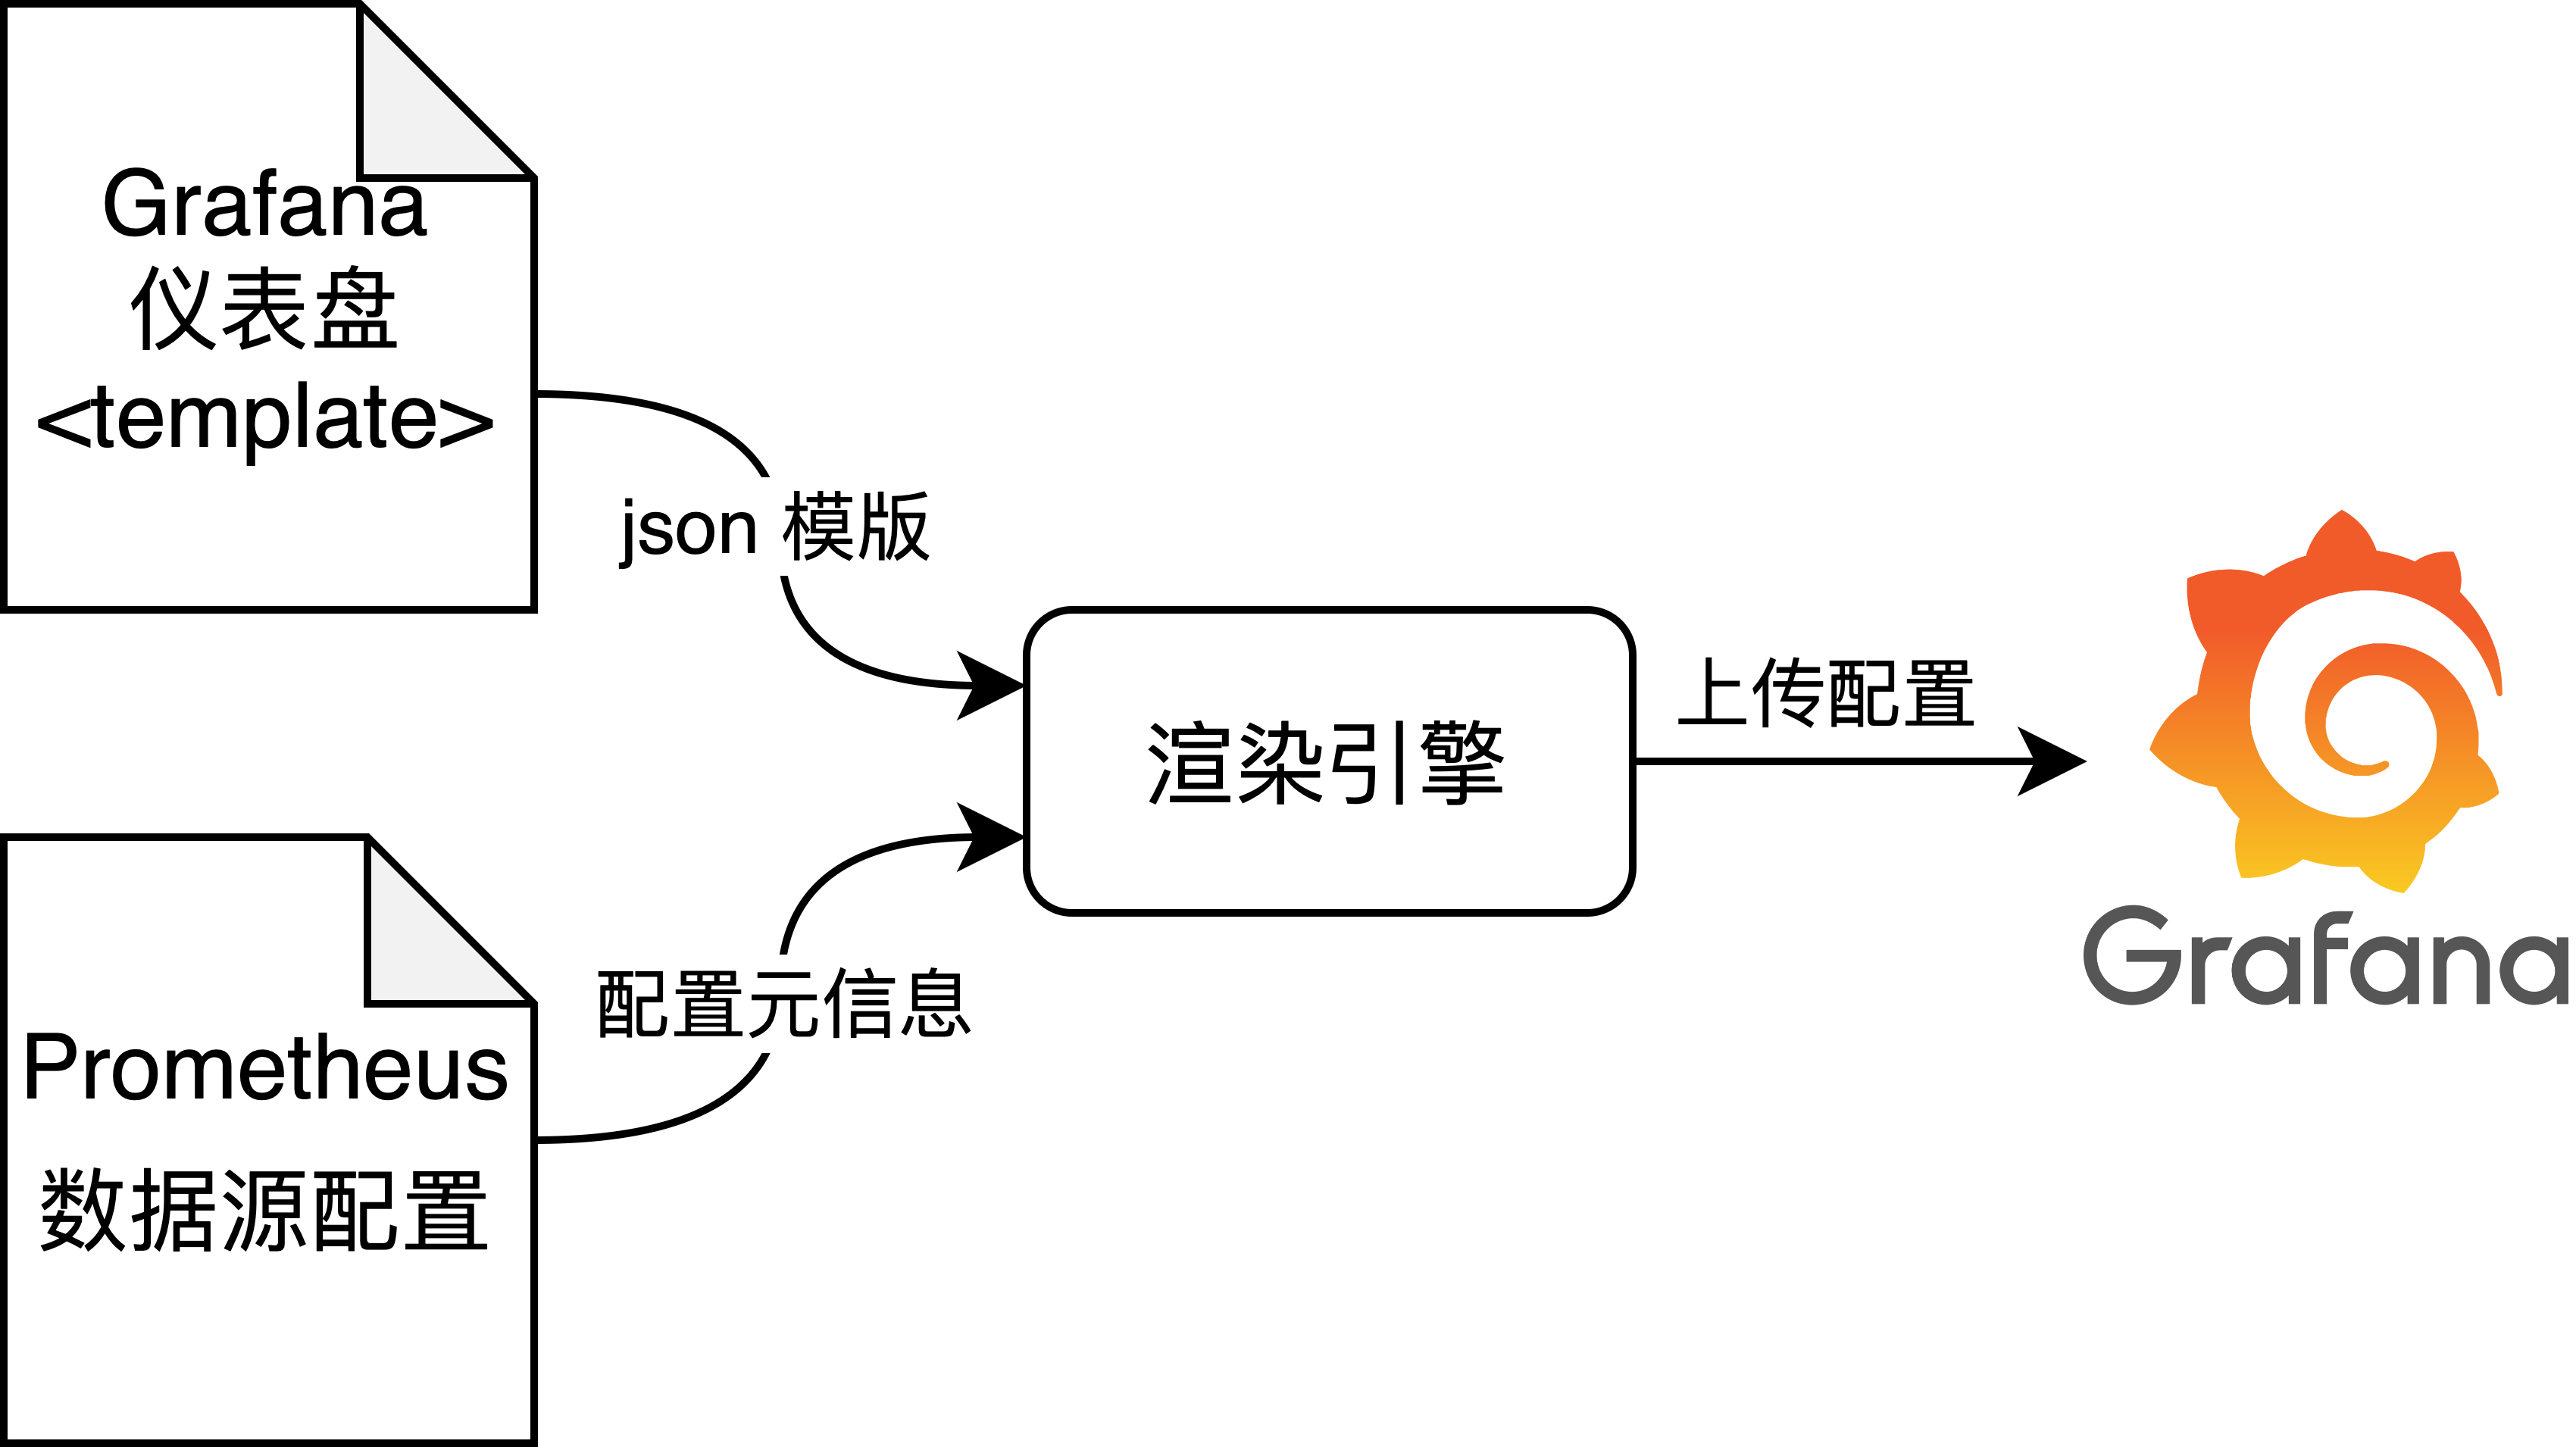
\includegraphics[width=0.65\linewidth]{pics/4-12grafana.png}
  \caption{监控数据可视化架构}
  \label{fig:4-12grafana}
\end{figure}

边缘节点的监控数据通过每一层的边缘节点逐步汇总,最终传输至云端。这一过程不仅有效减少了云边之间的冗余数据传输开销,还为边缘侧的实时调度提供了必要的数据支持。在云端,本文集成了Prometheus和Grafana数据可视化平台。如图\ref{fig:4-12grafana}所示,收集到的数据首先存储在Prometheus中。Prometheus作为一个强大的时间序列数据库,能够高效地存储和查询大量的监控数据。然后,通过预定义的Grafana仪表盘模板文件,填充相应的Prometheus数据源配置信息。这些模板文件包含了各种图表、面板和告警规则,可以根据实际需求进行灵活配置。最后,这些配置被上传到Grafana仪表盘,利用丰富的可视化组件提供直观的监控视图。这种可视化的方式使得相关人员能够快速掌握系统的运行状态,及时发现并处理潜在的问题,从而提高系统的整体可靠性和性能。

\section{本章小结}

本章介绍了云边协同AI推理调度系统的设计与实现。首先,详细阐述了KubeEdge及相关技术,包括其架构设计、设备管理机制以及EdgeMesh的服务通信机制。接着,对系统的整体架构进行了说明,明确了各组件在系统中的功能定位及其相互协作关系。最后,深入探讨了系统中各个关键组件的设计与实现细节,描述了这些组件如何为前文提出的调度算法提供系统支撑,从而确保云边协同环境下模型推理任务的高效调度与执行。



\chapter{实验设计与评估}

本章旨在全面评估本文提出的面向模型推理的云边协同调度算法及 KEAS 系统的有效性。实验设计分为三个部分:核心算法仿真实验、系统功能验证实验和系统性能评估实验。首先,核心算法仿真实验重点验证分层调度优化算法的性能表现。本文通过仿真模拟了云边环境中的计算节点以及设备流式数据的生成过程,并以最关键的服务质量指标(QoS)作为评估标准,包括边缘设备调度成功率和设备请求调度成功率。实验结果定量分析了分层委托调度算法在保证设备完整调度方面的显著优势,充分体现了其在复杂云边场景下的适用性和高效性。其次,系统功能验证实验主要测试 KEAS 系统中各核心模块的功能完整性。具体而言,实验针对模型推理服务以及系统监控服务模块进行了功能性验证,确保各模块能够稳定运行并协同工作,为系统的整体性能提供可靠保障。最后,系统性能评估实验深入分析了分层调度决策对响应时间的影响,实验验证了调度算法在负载均衡方面的有效性。结果表明,分层调度策略能够根据各计算节点的实时负载状态动态分配任务,从而在不同节点间实现任务负载的合理分布。

\section{实验配置}

\subsection{仿真实验配置}

为了评估第三章提出的调度优化算法的独立效果,本文设计并实现了一个轻量级的仿真实验平台。该仿真模块基于 Python 开发,旨在模拟云边协同系统中的任务卸载决策过程。本文假设系统中包含 2 个云节点、50 个边缘节点以及 100 个终端设备。每个终端设备由一个边缘节点的设备管理器控制,其任务生成频率在 $ [1, 10] $ Hz 的范围内递增。终端设备仅负责在每个时隙开始时生成任务,而不具备本地计算能力。生成的任务需要通过调度器完成任务卸载决策,任务卸载的目标范围包括:本地边缘节点、同一边缘集群内的其他边缘节点、不同边缘集群的边缘节点以及远端的云节点。由于在工业生产场景中获取真实的工业任务数据集较为困难,本文选择通过仿真平台生成模拟任务数据,参考 KubeEdge 的数据采集方式,设备管理器根据预设的采集频率,在每个时隙开始时触发终端设备的数据采集操作。这种基于仿真的工业任务生成方式,为任务卸载决策性能的评估与优化提供了可靠的基础。表 \ref{tab:simulation-parameters} 列出了实验仿真中使用的参数设置。

% 参数设置表格
\begin{table}[ht]
    \renewcommand{\arraystretch}{1.5}
    \centering
    \caption{仿真参数设置}
    \label{tab:simulation-parameters}
    \begin{tabular}{lll}
        \toprule
        \textbf{参数} & \textbf{设置} \\
        \midrule
        终端设备数量 & 100 \\
        边缘节点数量 & 50 \\
        边缘层级数量 & 2 \\
        边缘子树数量 & 5 \\
        云端节点数量 & 5 \\
        任务数据量 & $[100 \, \text{KB}, 500 \, \text{KB}]$ \\
        边缘节点计算能力 & $2 \, \text{GHz}$ \\
        边缘节点间传输速率 & $1 \, \text{Gbps}$ \\
        边缘与云传输速率 & $128 \, \text{Mbps}$ \\
        \bottomrule
    \end{tabular}
\end{table}

为了更好地模拟工业场景中的实际需求,本文选用目标检测模型作为任务的核心计算负载。目标检测是工业界常见的应用场景之一,广泛应用于智能监控、缺陷检测和自动化流水线等领域。表 \ref{tab:model-flops} 提供了常用目标检测模型的 FLOPs 数据,用于后续分析任务计算复杂度。

% FLOPs 数据表格
\begin{table}[ht]
    \renewcommand{\arraystretch}{1.5}
    \centering
    \caption{常见目标检测模型处理单张图像的 FLOPs 数据}
    \label{tab:model-flops}
    \begin{tabular}{lll}
        \toprule
        \textbf{模型名称} & \textbf{FLOPs} \\
        \midrule
        YOLOv3\cite{redmon2018yolov3} & $65.86 \, \text{GFLOPs}$ \\
        YOLOv3-tiny & $5.58 \, \text{GFLOPs}$ \\
        YOLOv4\cite{wang2021scaled} & $109.25 \, \text{GFLOPs}$ \\
        YOLOv4-tiny\cite{gu2022novel} & $6.97 \, \text{GFLOPs}$ \\
        YOLOv5s & $16.51 \, \text{GFLOPs}$ \\
        YOLOv5-tiny & $3.49 \, \text{GFLOPs}$ \\
        \bottomrule
    \end{tabular}
\end{table}

\subsection{系统实验配置}

本实验环境基于两台 X86 架构的物理服务器和一台配备 NVIDIA RTX 3080 GPU 的高性能服务器构建。其中,配备 RTX 3080 GPU 的服务器充当云端节点。每台物理服务器上部署了 libvirt 虚拟化管理平台,通过QEMU/KVM技术构建跨主机虚拟机集群,从而实现异构计算资源的统一调度与高效管理。为了模拟真实的云边协同场景,本文利用 Open vSwitch 创建虚拟网卡,并在路由器上配置相关路由规则,从而实现虚拟机之间的互联互通。通过限制虚拟网络接口的带宽和延迟,本文能够精确模拟不同网络条件下的云边通信环境。实验环境的整体架构如图\ref{fig:5-1all}所示。

\begin{figure}[ht]
  \centering
  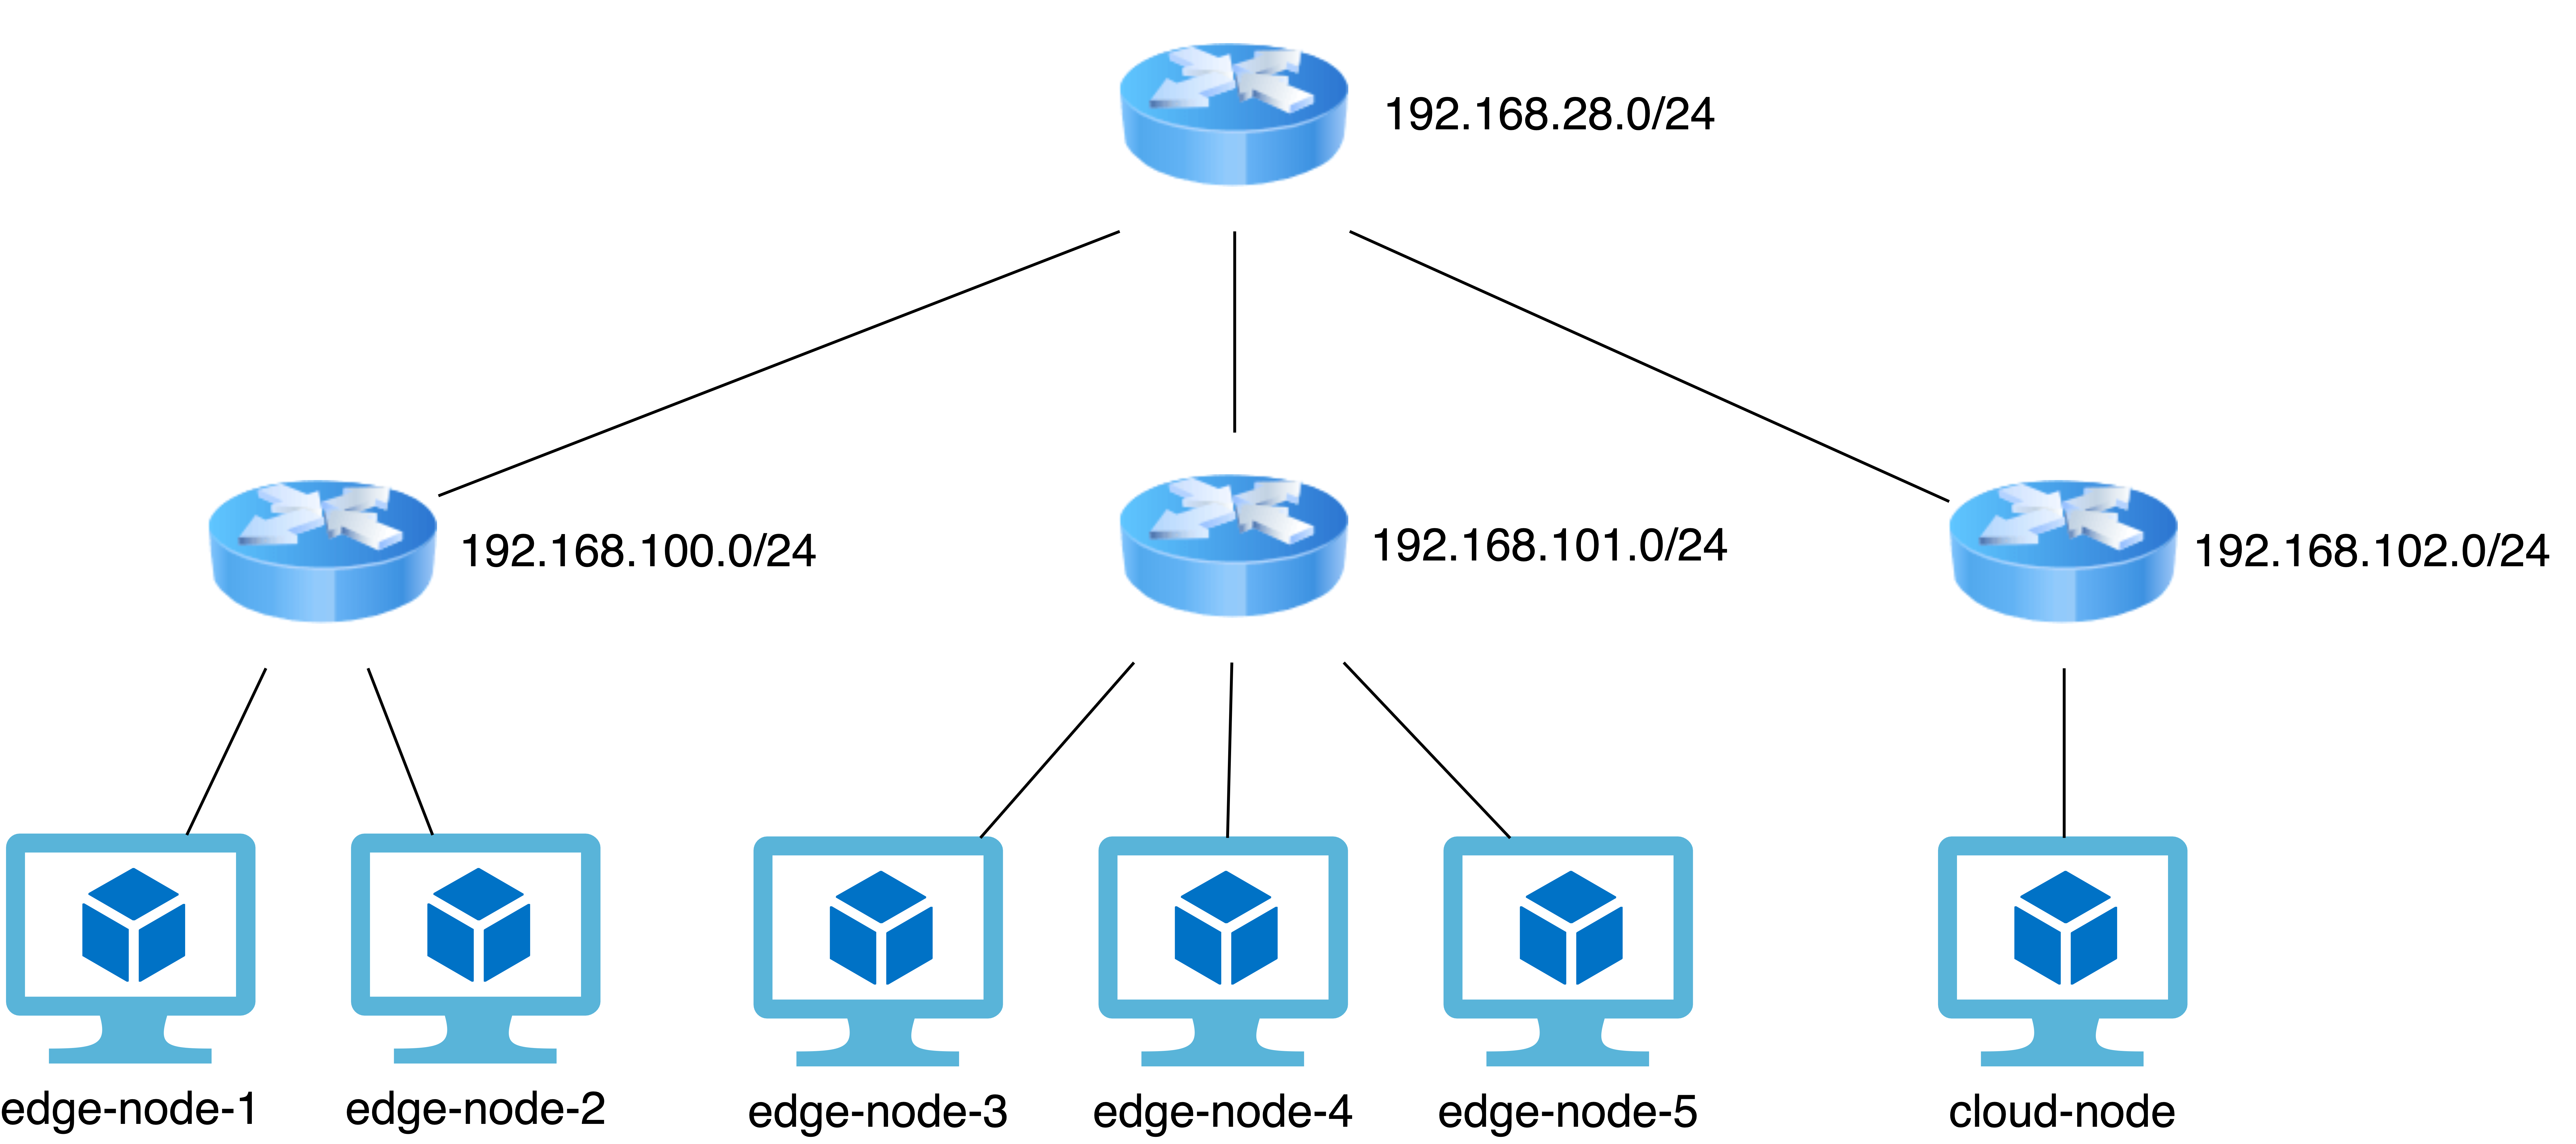
\includegraphics[width=\linewidth]{pics/5-1all.png}
  \caption{系统实验环境网络拓扑图}
  \label{fig:5-1all}
\end{figure}

具体配置参数如表\ref{tab:vm-configurations}所示。

\begin{table}[ht]
    \centering
    \renewcommand{\arraystretch}{1.2}
    \caption{实验环境虚拟化节点配置}
    \label{tab:vm-configurations}
    \begin{tabular}{cccccccc}
        \toprule
        \textbf{序号} & \textbf{设备名称} & \textbf{CPU} & \textbf{内存} & \textbf{系统} & \textbf{架构} & \textbf{IP地址} & \textbf{子网掩码} \\
        \midrule
        1 & edge-node-1 & 2核 & 4GB & Ubuntu 22.04 & amd64 & 192.168.100.1 & 255.255.255.0 \\
        2 & edge-node-2 & 4核 & 8GB & Ubuntu 22.04 & amd64 & 192.168.100.2 & 255.255.255.0 \\
        3 & edge-node-3 & 2核 & 4GB & Ubuntu 22.04 & amd64 & 192.168.101.1 & 255.255.255.0 \\
        4 & edge-node-4 & 2核 & 4GB & Ubuntu 22.04 & arm32 & 192.168.101.2 & 255.255.255.0 \\
        5 & edge-node-5 & 2核 & 4GB & Ubuntu 22.04 & arm64 & 192.168.101.3 & 255.255.255.0 \\
        6 & cloud-node & 8核 & 32GB & Ubuntu 22.04 & amd64 & 192.168.102.1 & 255.255.255.0 \\
        \bottomrule
    \end{tabular}
    \vspace{6pt}
\end{table}

本文的系统实验基于 KubeEdge 搭建,并选择目标检测作为核心任务负载,以评估调度算法在实际工业场景中的性能表现。为了生成目标检测任务所需的数据流,本文在 Ubuntu 系统上创建了虚拟的 USB 摄像头设备。具体而言,本文利用 Linux 内核模块 \texttt{v4l2loopback} 创建虚拟视频设备,该模块能够模拟真实的摄像头输入,并支持多种分辨率和帧率设置,从而为实验提供多样化且可控的数据源。进一步地,通过 FFmpeg 工具生成合成视频流并将其绑定到虚拟视频设备,确保数据流的稳定性与一致性。此外,借助 KubeEdge 的设备管理接口 DMI,动态调整虚拟设备的采集频率和数据大小,灵活配置实验参数。图 \ref{fig:dmi-config} 展示了部分 DeviceModel 配置文件。

\begin{figure}[ht]
    \centering
    \begin{lstlisting}[
        language=YAML,
        basicstyle=\small\ttfamily, 
        numbers=left, % 可选:添加行号
        numberstyle=\tiny\color{gray}, % 可选:行号样式
        frame=shadowbox
    ]
apiVersion: devices.kubeedge.io/v1beta1
kind: DeviceModel
metadata:
  name: camera-usb
  namespace: default
spec:
  protocol: camera-usb
  properties:
    - name: Framerate
      description: Framerate
      type: FLOAT
      accessMode: ReadWrite
    - name: Brightness
      description: Brightness
      type: INT
      accessMode: ReadWrite
      maximum: "127"
      minimum: "-127"
    - name: Contrast
      description: Contrast
      type: INT
      accessMode: ReadWrite
      maximum: "511"
      minimum: "0"
    ...
\end{lstlisting}
    \caption{USB 摄像头设备管理器部分配置文件}
    \label{fig:dmi-config}
\end{figure}

\section{核心算法仿真实验}

\subsection{调度优化算法比较}

本文将提出的分层调度优化算法与以下基准算法进行对比分析,这些算法在工业界中具有一定的代表性,具体描述如下:

\begin{enumerate}
    \item \textbf{全部本地执行算法(All Local Execution,ALE)}:所有的设备流式数据都在本地执行,不需要卸载。
    \item \textbf{随机卸载算法(Random Offloading Algorithm)}:该算法通过随机选择卸载目标节点来分配任务。
    \item \textbf{轮询卸载算法(Round-Robin Algorithm)}:该算法按照固定的顺序依次分配任务到不同的边缘或云端节点。
\end{enumerate}

本文最大的服务质量(QoS)指标是边缘设备调度成功率和设备请求调度成功率,其中边缘设备调度成功率指边缘设备生成的流式数据能够被完整处理的比例,该指标反映了系统对边缘设备任务的整体处理能力;设备请求调度成功率指设备生成的流式数据中成功被处理的比例,该指标更关注单个任务请求的完成情况,尤其是在高负载场景下的表现。

本文通过对比实验对于 EdgeMesh 网关提供的轮询卸载和随机卸载方法,在高请求率场景下表现出明显的性能不足。具体而言,当任务到达率超过系统处理能力时,这两种方法往往会出现显著的丢包现象和响应延迟增加的问题。随机卸载算法由于缺乏对节点负载状态的感知,随机选择卸载目标可能导致部分节点过载,而其他节点资源闲置,从而降低整体调度效率。轮询卸载算法尽管通过固定顺序分配任务能够在一定程度上平衡负载,但其静态调度策略无法适应动态变化的网络环境和突发流量,导致在高请求率下性能急剧下降。

\begin{figure}[ht]
    \centering
    \begin{subfigure}{\textwidth}
        \centering
        \begin{subfigure}{0.48\textwidth}
            \centering
            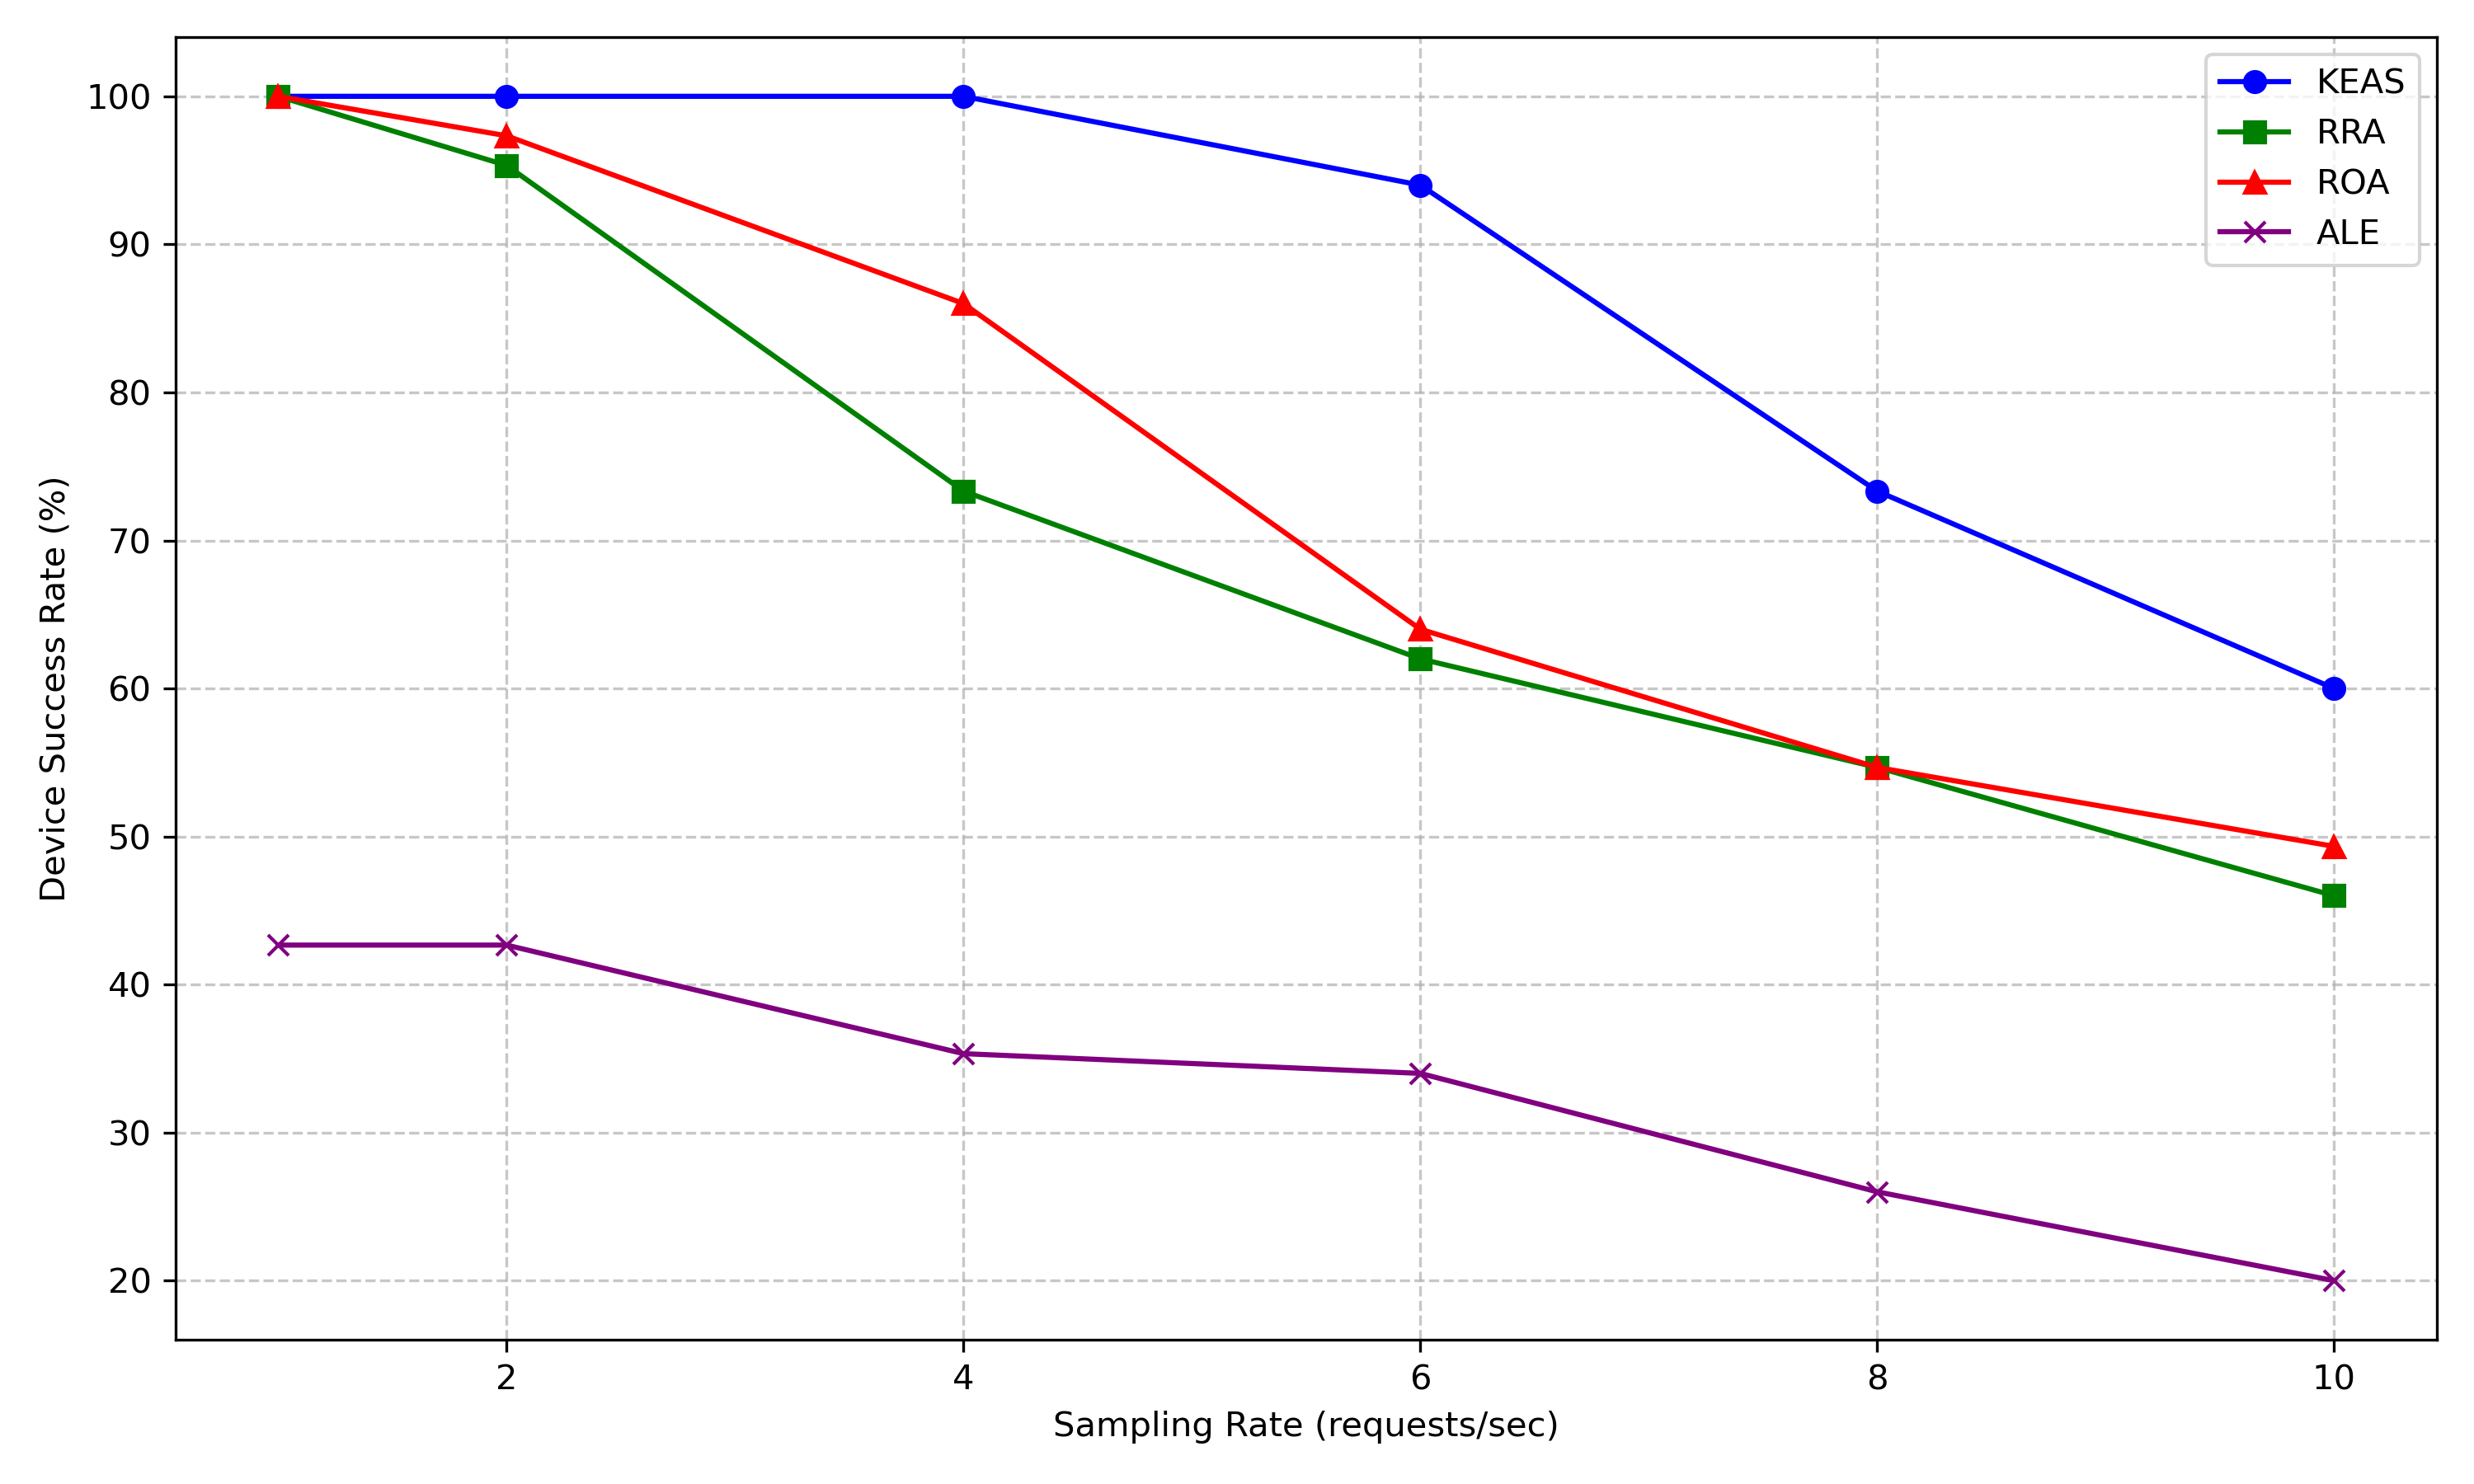
\includegraphics[width=\linewidth]{pics/expr/exp9_device_success_rate.png}
            \caption{边缘设备调度成功率}
            \vspace{0.3cm}
        \end{subfigure}
        \begin{subfigure}{0.48\textwidth}
            \centering
            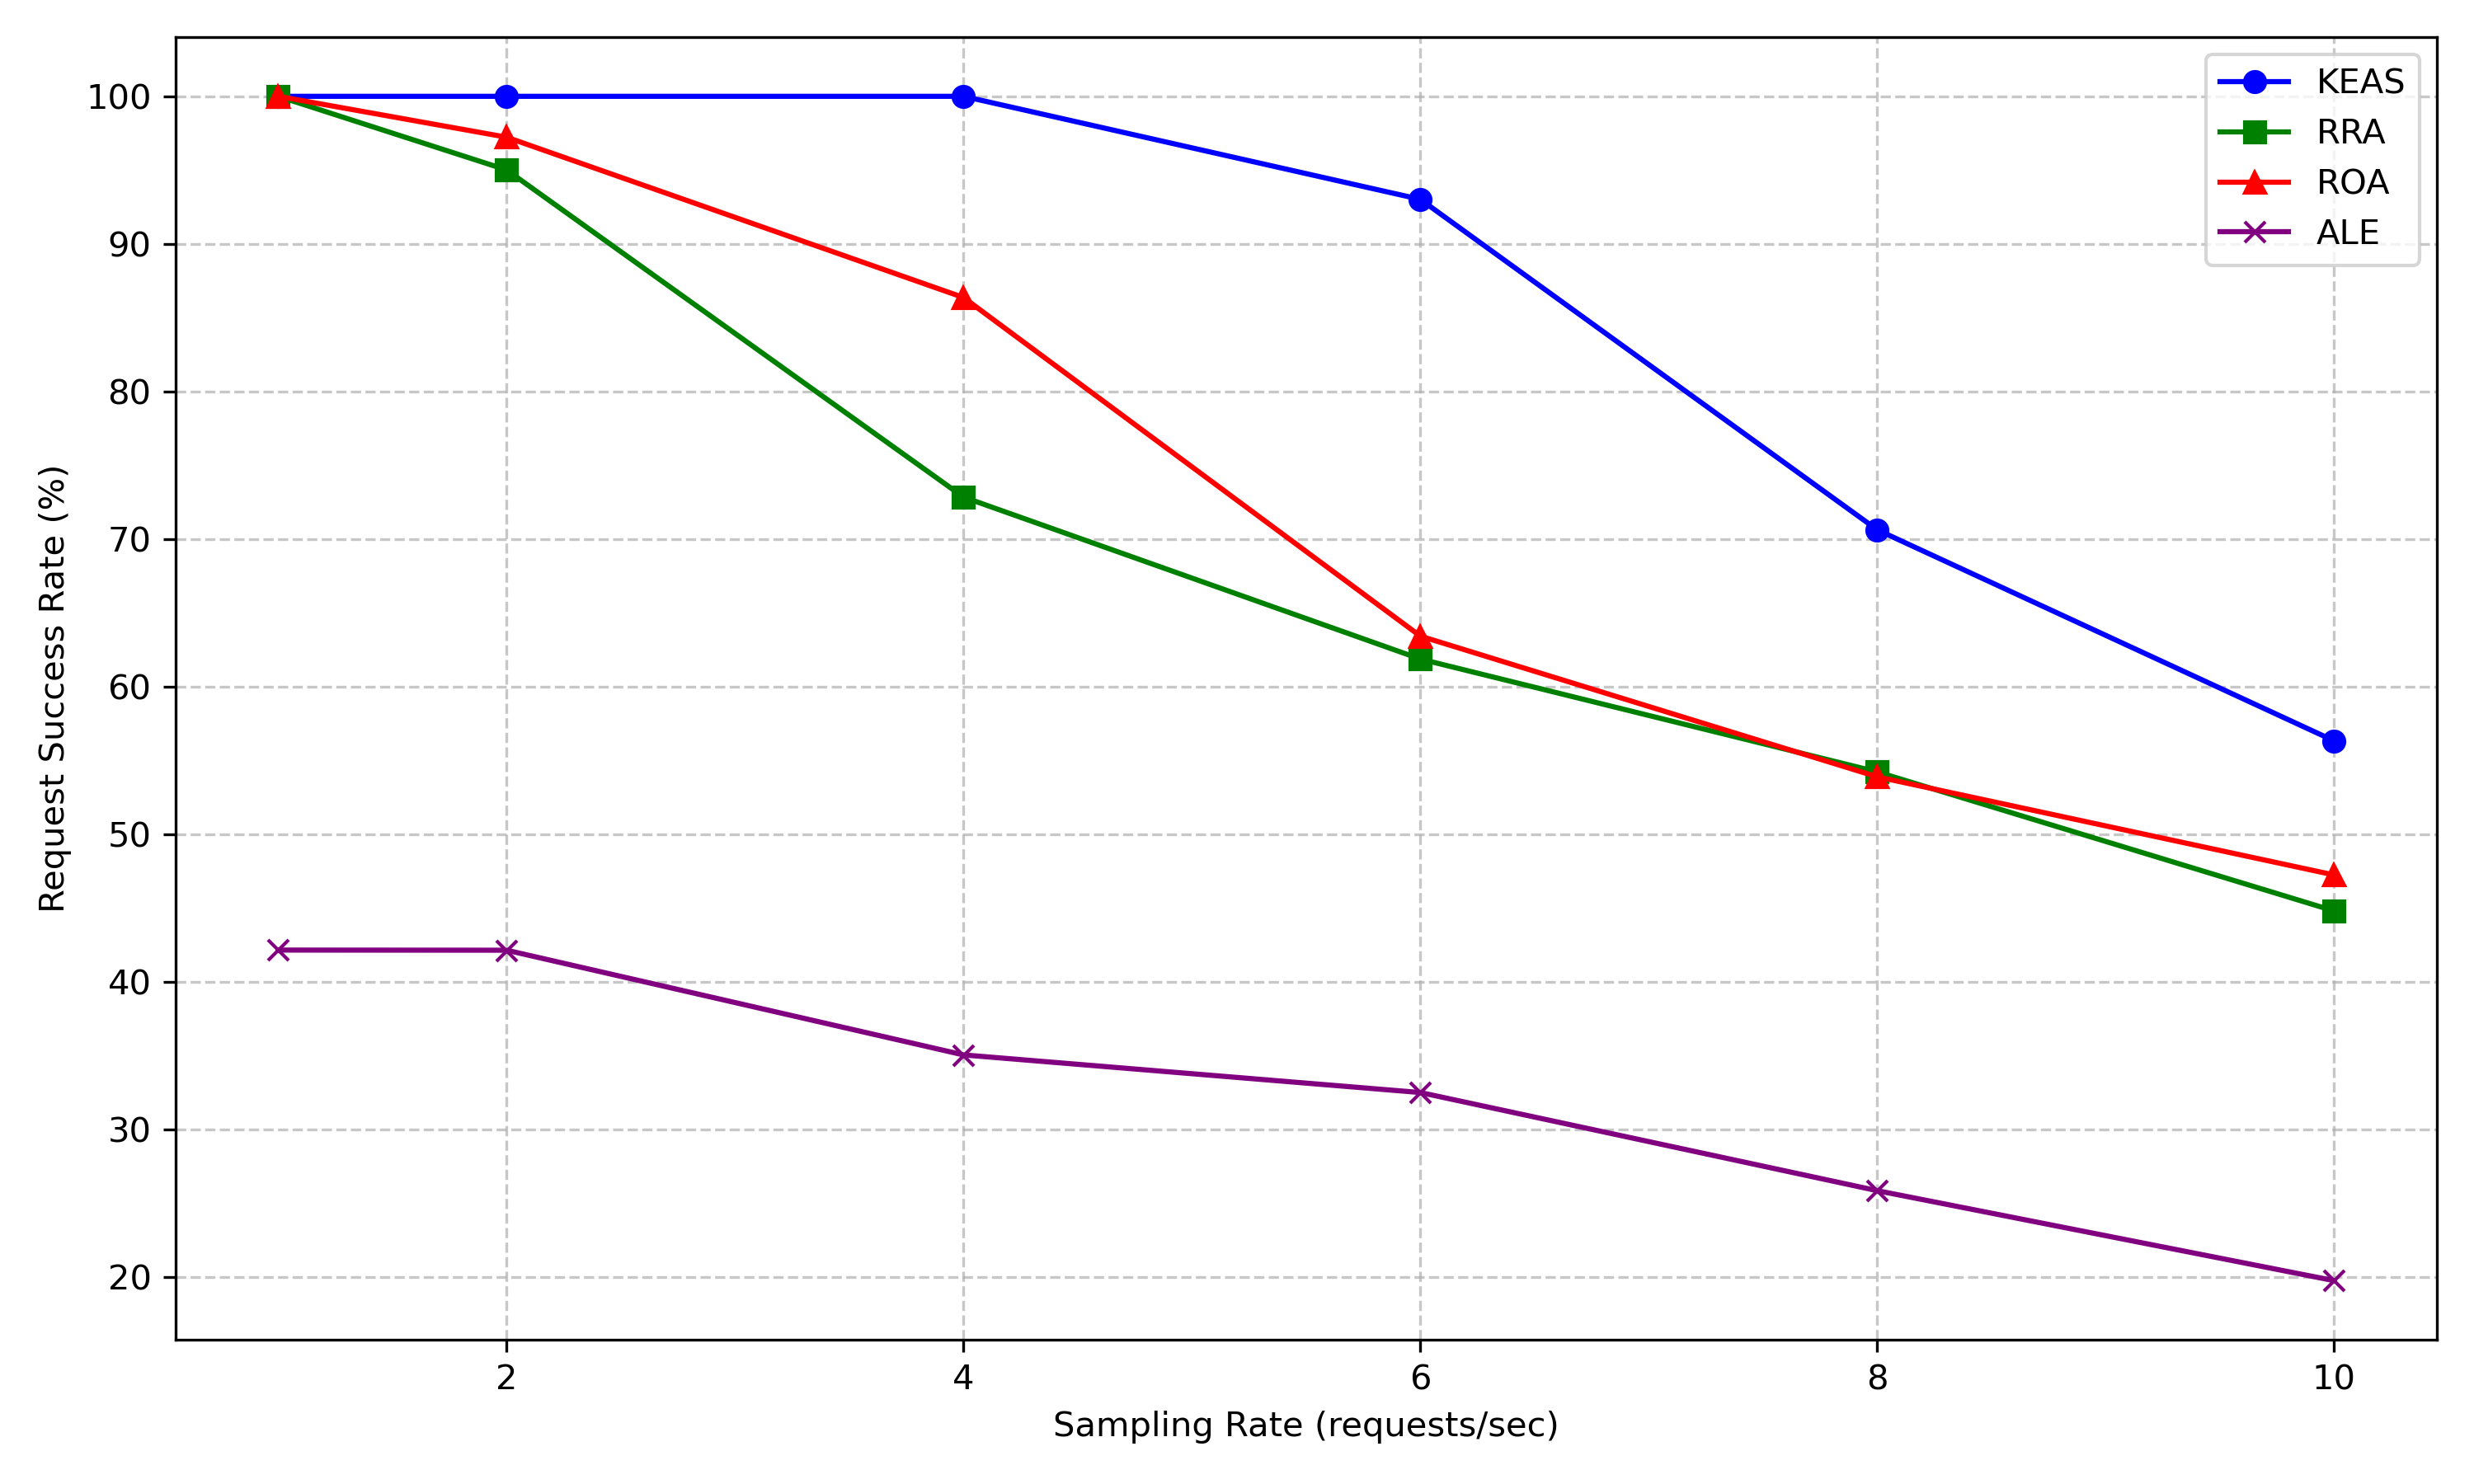
\includegraphics[width=\linewidth]{pics/expr/exp9_request_success_rate.png}
            \caption{设备请求调度成功率}
            \vspace{0.3cm}
        \end{subfigure}
    \end{subfigure}
    \caption{不同调度策略的服务质量对比}
    \label{fig:exp1}
\end{figure}

\subsection{分层调度器实验分析}

本文针对每一层级的调度设计了相应的优化算法,这些算法分别针对不同的优化目标展开。为了评估这些优化算法的实际效果,本文对每一层级调度器所采用的优化算法进行了实验分析,旨在比较不同优化方式在各层级调度中的性能表现及其适用性。

\subsubsection{边缘节点调度器实验分析}

\begin{figure}[ht]
    \centering
    \begin{subfigure}{\textwidth}
        \centering
        \begin{subfigure}{0.48\textwidth}
            \centering
            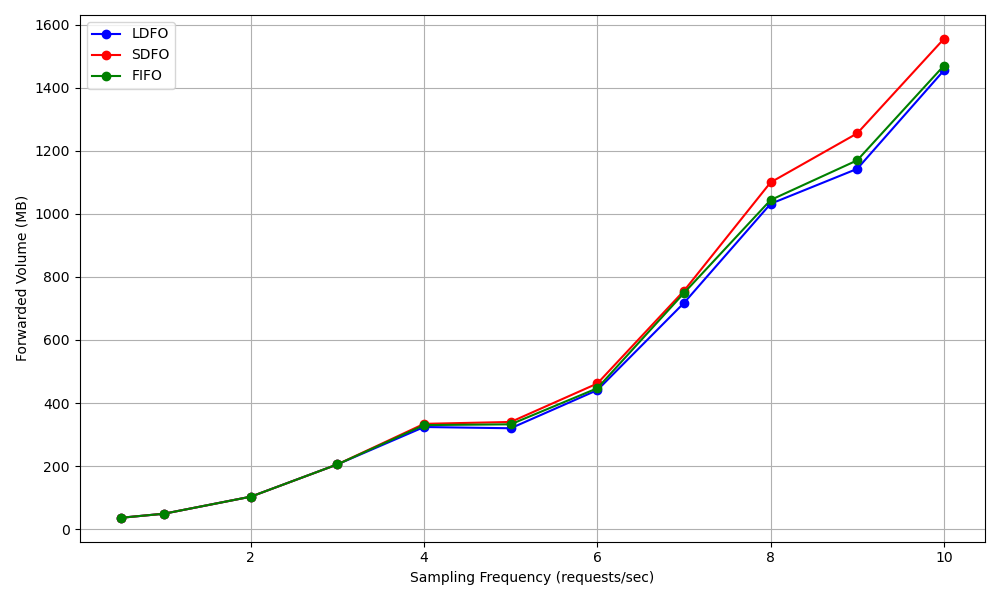
\includegraphics[width=\linewidth]{pics/expr/exp3_frequency_forwarded.png}
            \caption{跨节点协作总流量}
            \vspace{0.3cm}
        \end{subfigure}
        \begin{subfigure}{0.48\textwidth}
            \centering
            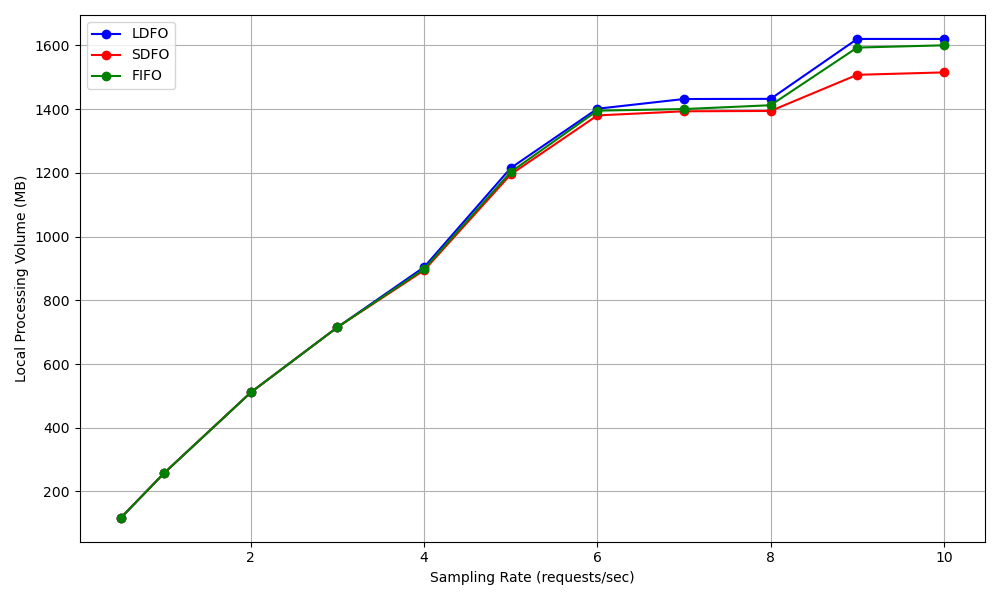
\includegraphics[width=\linewidth]{pics/expr/exp3_frequency_local_processed.png}
            \caption{本地处理的数据总流量}
            \vspace{0.3cm}
        \end{subfigure}
    \end{subfigure}
    \caption{不同优化策略下的本地调度性能对比}
    \label{fig:exp2}
\end{figure}

在边缘节点调度调度层次,本文重点比较了三种常见的队列优化策略:先进先出(First In First Out,FIFO)、最小数据量优先(Small Data First Out,SDFO)以及最大数据量优先(Large Data First Out,LDFO)。实验在相同的配置条件下进行,仅通过调整数据采集频率来观察三种优化策略的表现差异。如图 \ref{fig:exp2} 所示,实验结果表明,在边缘节点调度策略中,本文所用的LDFO 方式能够在保证本地设备数据流处理量的同时,有效减少跨节点协作流量,并最大化本地节点处理的数据总流量。这一策略显著提升了本地节点的资源利用率和整体调度效率,体现了其在高负载场景下的优越性。

\subsubsection{云端调度器实验分析}

\begin{figure}[ht]
  \centering
  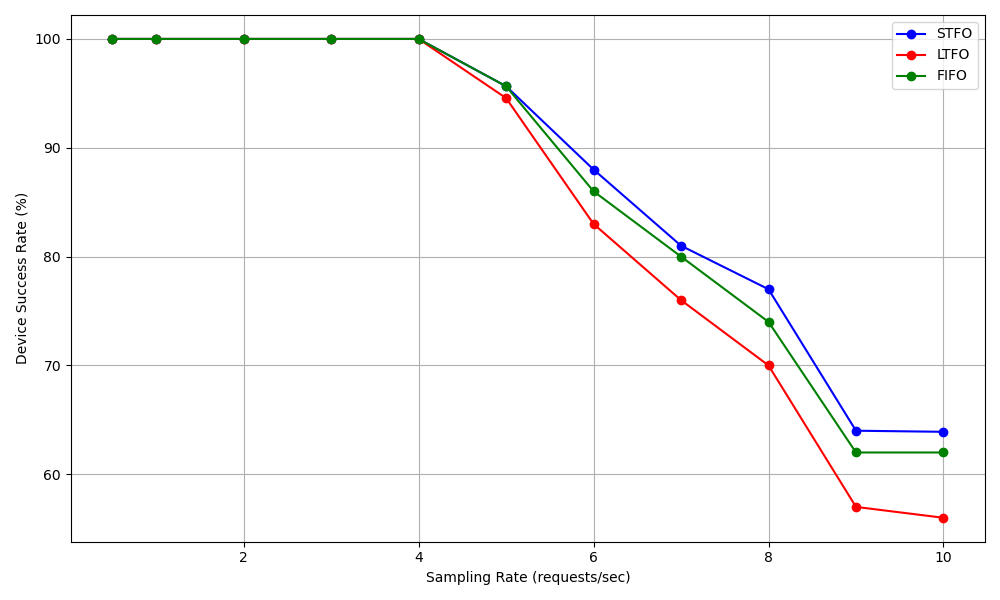
\includegraphics[width=0.8\linewidth]{pics/expr/exp5_frequency_device_success_rate.png}
  \caption{不同优化队列下的全局调度设备成功率}
  \label{fig:exp4}
\end{figure}

在云端调度层次,本文比较了三种常见的队列优化策略:最小任务优先(Small Task First Out, STFO)、最大任务优先(Large Task First Out, LTFO)以及先来先服务(First-Come, First-Served, FCFS)。实验在相同的配置条件下进行,仅通过调整数据采集频率来观察三种队列的表现差异。由于本实验中云端资源是有限的,因此会出现任务失败的情况。如图 \ref{fig:exp4} 所示,实验结果表明,在云端全局调度策略中,本文所用的 STFO 方式能够显著提高设备的任务成功率。

\section{系统功能验证实验}

\subsection{模型推理实例动态部署功能验证}

为了验证模型推理实例动态部署功能的有效性,我们设计了一组实验,在多种架构的机器上利用 KEAS 实现目标监测模型的部署,并评估其运行准确性和适配能力。表\ref{tab:multi-arch-zhichi}展示了 KEAS 对四种主流架构的支持情况

\begin{table}[ht]
    \renewcommand{\arraystretch}{1.5}
    \centering
    \caption{KEAS对不同架构的机器的适配程度}
    \label{tab:multi-arch-zhichi}
    \begin{tabular}{|l|l|}
        \hline
        \textbf{架构类型} & \textbf{适配结果}  \\ \hline
        ARM32 (32-bit) & 支持 \\ \hline
        ARM64 (64-bit) & 支持 \\ \hline
        AMD64 & 支持 \\ \hline
        AMD64 (no-AVX2) & 支持 \\ \hline
    \end{tabular}
\end{table}

实验结果表明,KEAS 的部署模块能够成功支持在多种架构的机器上部署模型推理实例。在每个部署任务完成后,TensorFlow Serving 的运行日志关键部分均如图\ref{fig:aiapply}所示。这进一步验证了 KEAS 在主流硬件架构上的适配能力和稳定性。

\begin{figure}[ht]
    \centering
    \begin{lstlisting}[
        basicstyle=\small\ttfamily, 
        frame=single
    ]
[INFO] Successfully loaded servable version 
{name: yolov4-tiny version: 1}
[INFO] Running gRPC ModelServer at 0.0.0.0:8500 ...
[INFO] Exporting HTTP/REST API at:localhost:8501 ...
\end{lstlisting}
    \caption{目标监测模型在 TensorFlow Serving 上的运行日志}
    \label{fig:aiapply}
\end{figure}

此外,我们还测试了不同深度学习框架之间的模型转换功能,并基于 YOLO 模型验证了其可行性。具体而言,实现了从 PyTorch、Keras 和 ONNX 到 TensorFlow 模型的转换,确保这些模型能够在 KEAS 系统中无缝集成和部署。表~\ref{tab:model-conversion-results} 展示了不同框架间模型转换的验证结果。

\begin{table}[ht]
    \renewcommand{\arraystretch}{1.5}
    \centering
    \caption{不同框架间模型转换的验证结果}
    \label{tab:model-conversion-results}
    \begin{tabular}{|l|l|l|}
        \hline
        \textbf{源框架} & \textbf{目标框架} & \textbf{转换结果} \\ \hline
        PyTorch & TensorFlow & 支持 \\ \hline
        Keras & TensorFlow & 支持 \\ \hline
        ONNX & TensorFlow & 支持 \\ \hline
    \end{tabular}
\end{table}


\subsection{模型推理实例批处理功能验证}

为验证模型推理实例批处理测试功能的有效性,并快速确定模型的最优批处理大小,同时为之前的仿真实验提供真实数据支撑,本文在系统运行过程中采集了批处理测试的相关数据,并分别测试了模型推理实例在 CPU 和 GPU 环境下的运行性能,以下给出 YOLOv4 模型的相关采集数据。

\begin{figure}[ht]
  \centering
  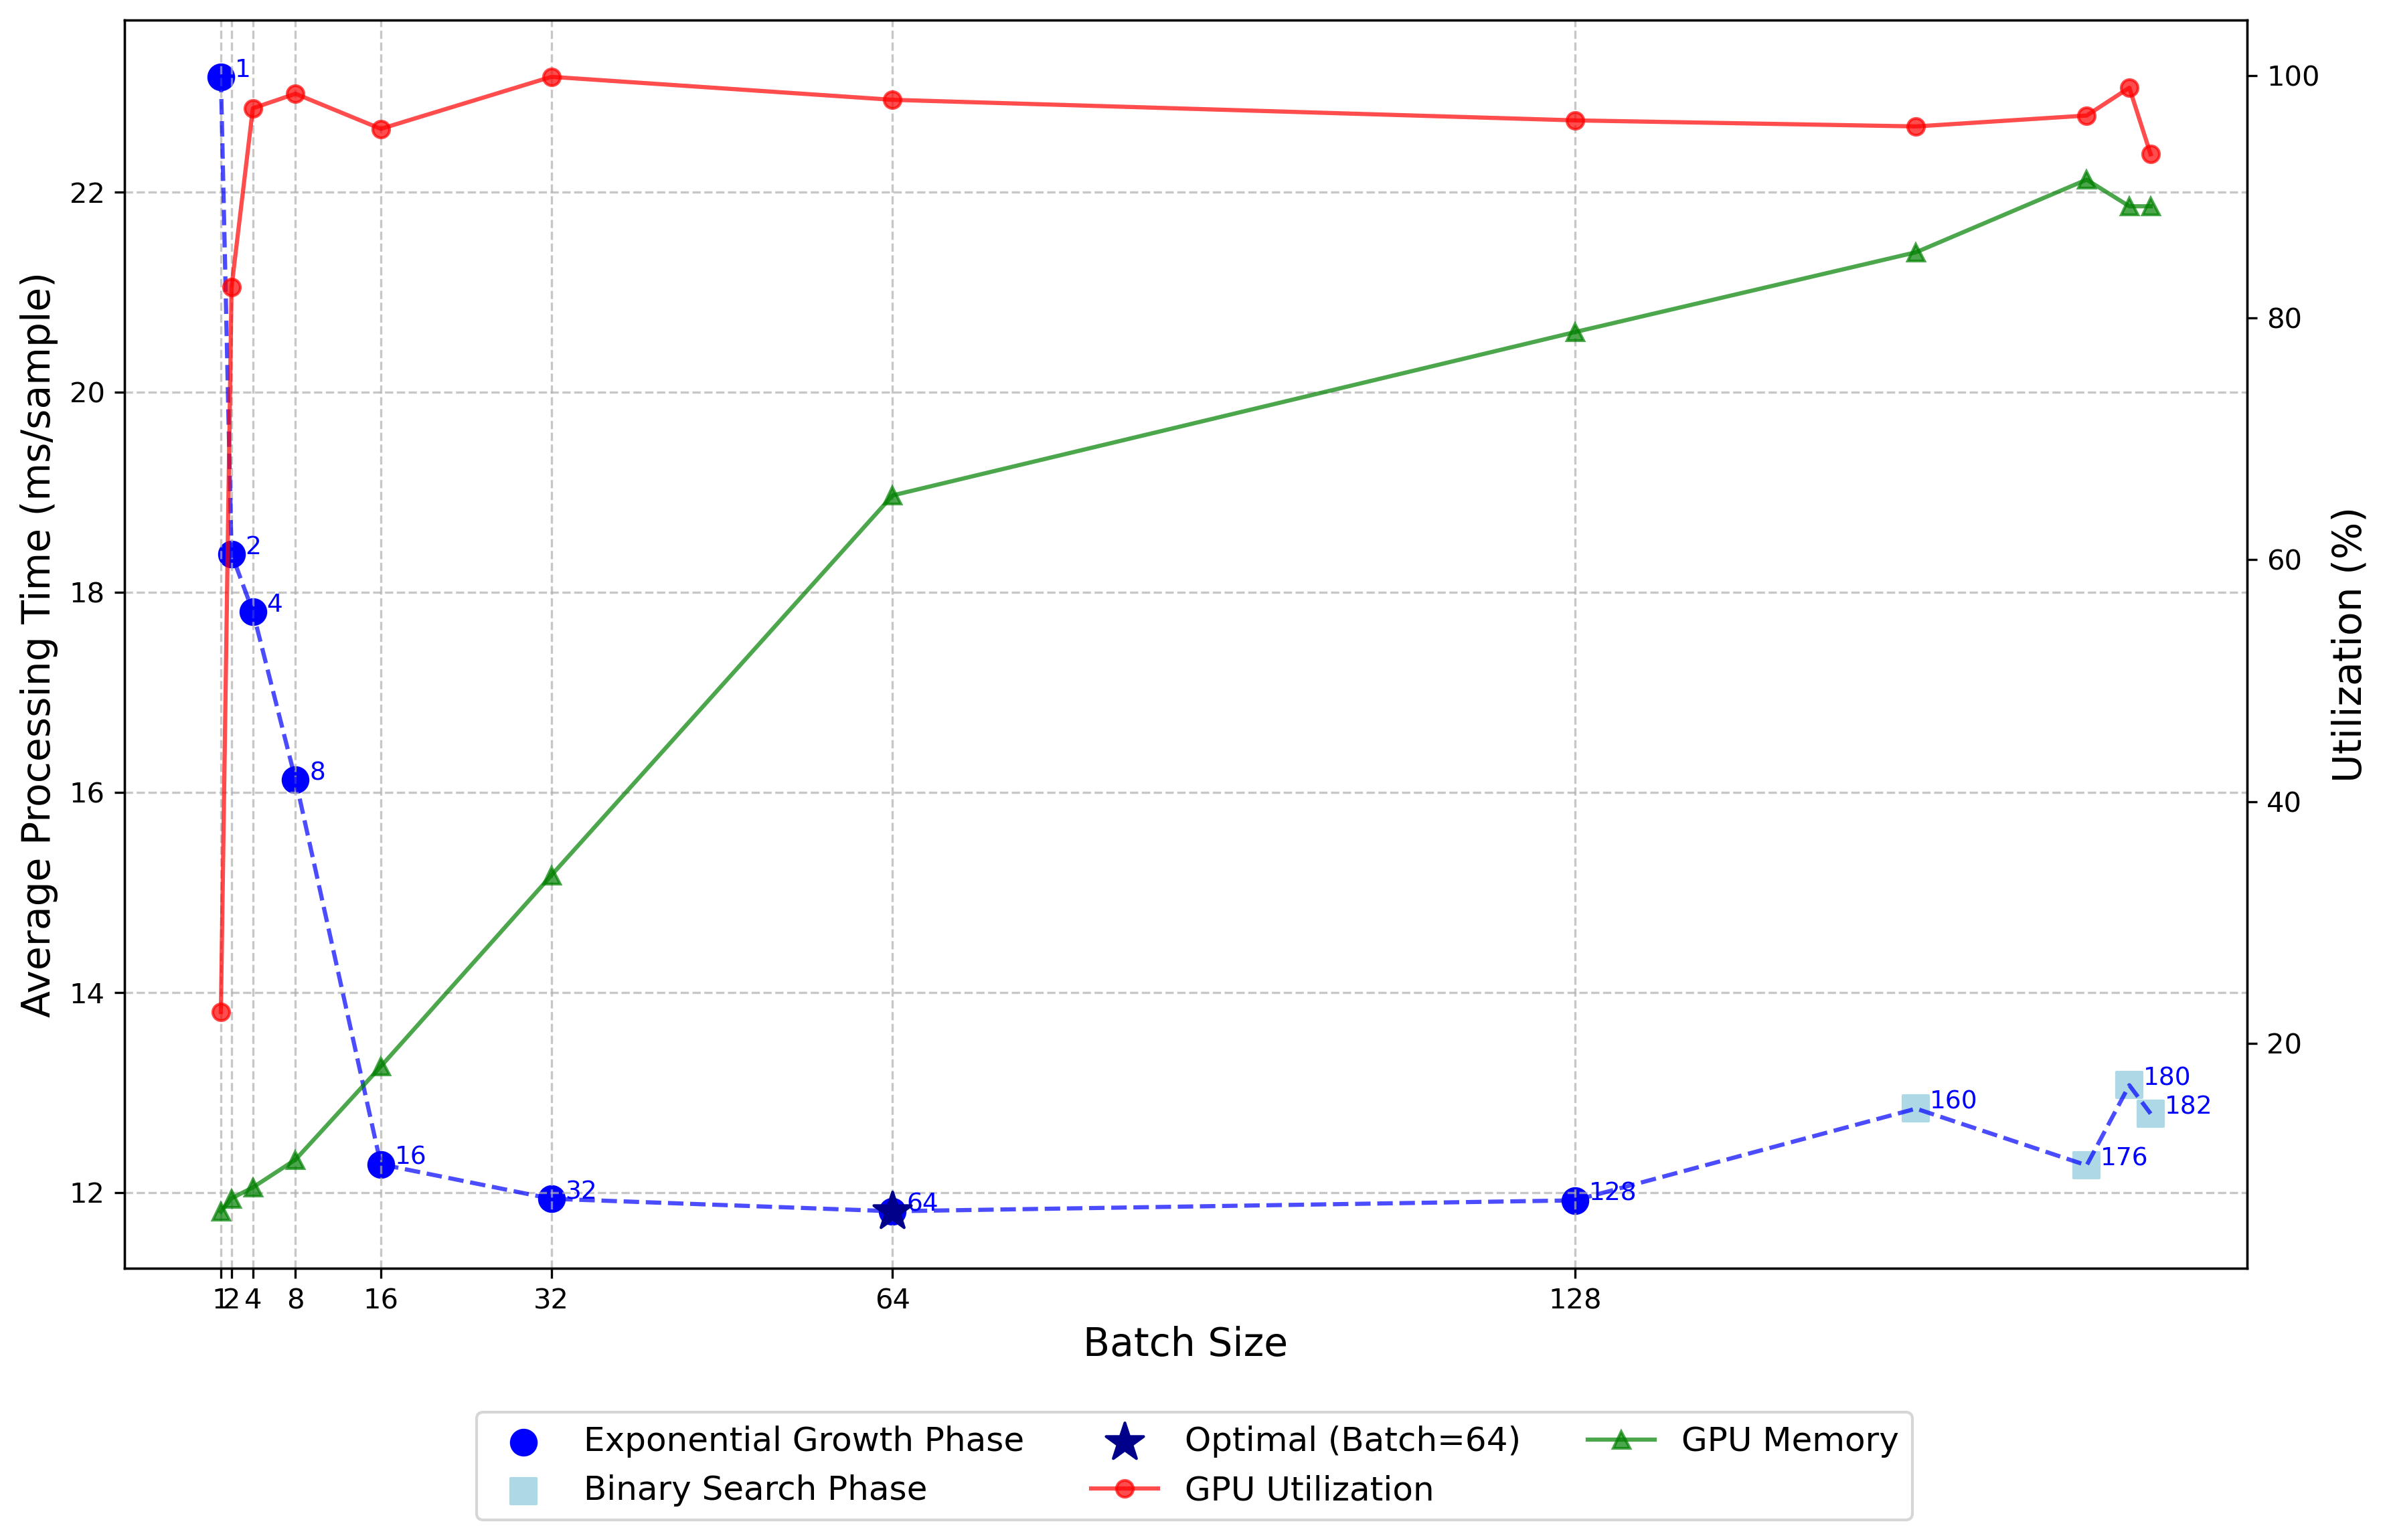
\includegraphics[width=0.8\linewidth]{pics/expr/yolov3_gpu_performance.png}
  \caption{GPU上的目标监测模型批处理性能分析}
  \label{fig:expaigpu}
\end{figure}

如图 \ref{fig:expaigpu} 所示,在 GPU 环境下运行 YOLOv4 相关模型时,随着批处理大小的增加,GPU 的利用率和显存占用呈现逐步上升的趋势。批处理规模的扩大使得更多的数据能够被并行加载到显存中进行计算,从而显著提高了 GPU 的计算资源利用率。然而,由于 GPU 显存容量的限制,当批处理大小达到一定阈值时,显存占用接近硬件上限,并最终因显存不足(Out of Memory, OOM)而无法继续扩展批处理规模。实验结果表明,在该显卡配置下,YOLO 模型在稳定运行状态下平均处理一张图片所需时间为 11.8 毫秒。

\begin{figure}[ht]
  \centering
  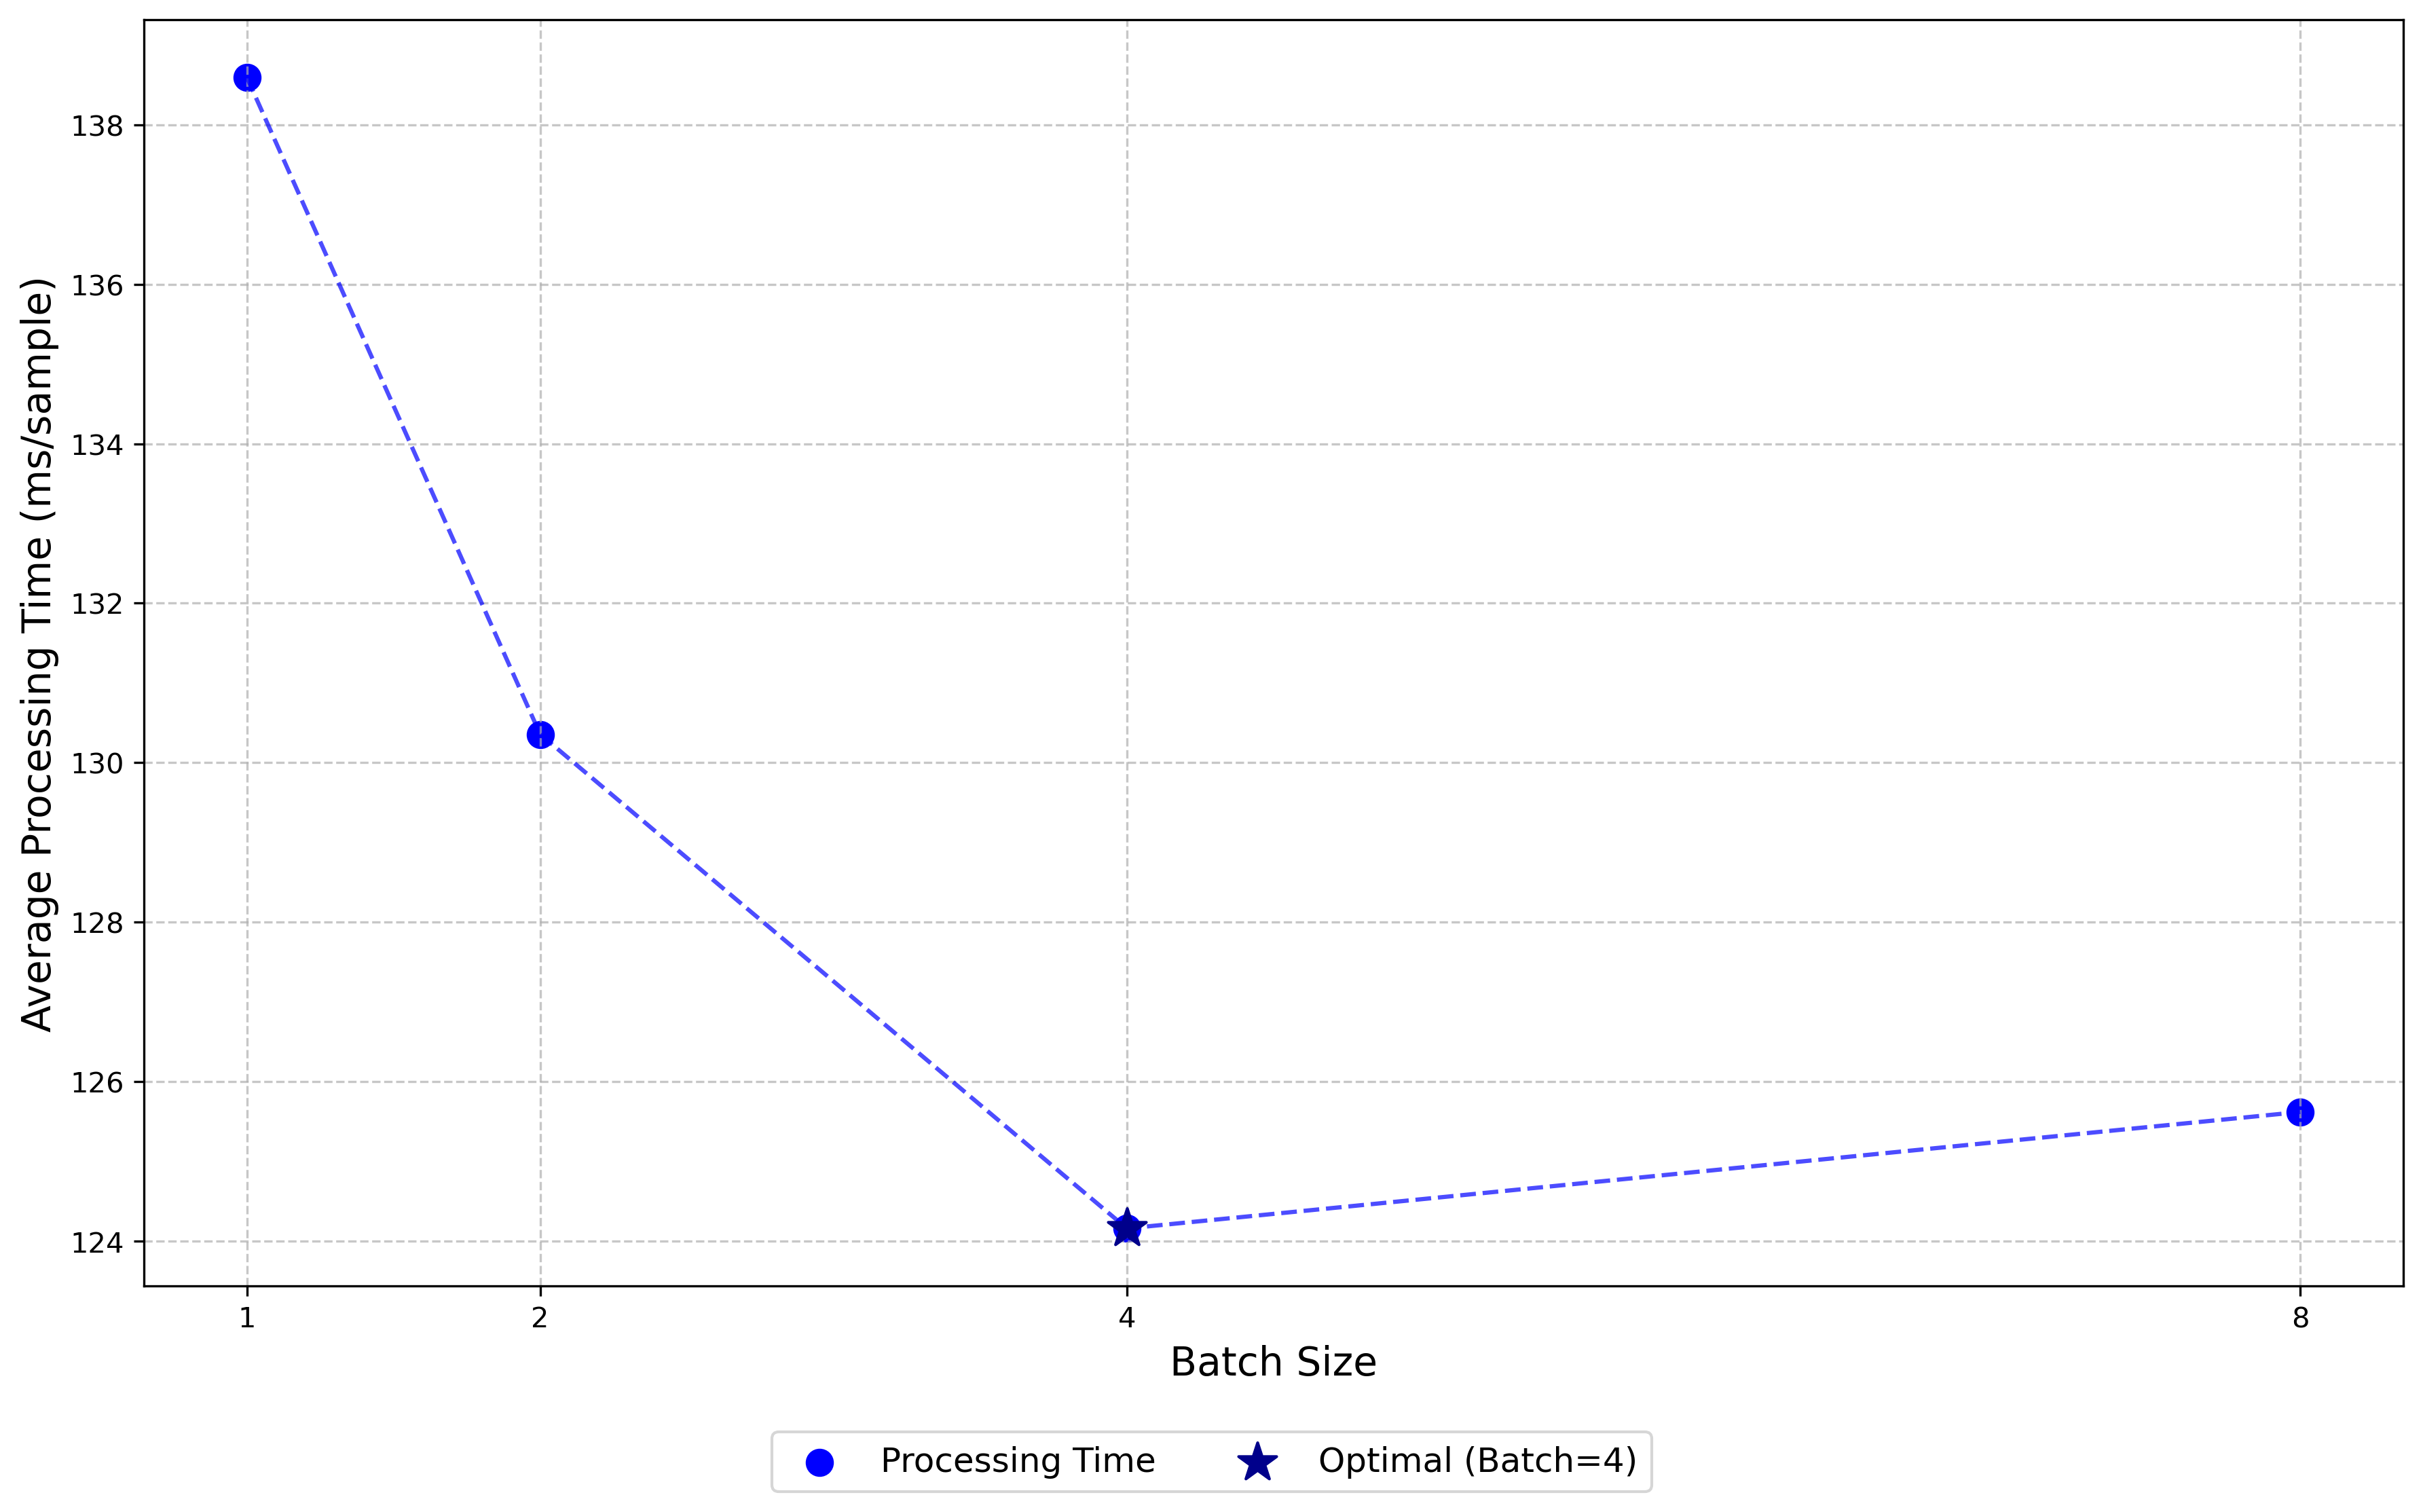
\includegraphics[width=0.8\linewidth]{pics/expr/yolov3_cpu_performance.png}
  \caption{CPU上的目标监测模型批处理性能分析}
  \label{fig:expaicpu}
\end{figure}

与GPU的众核架构不同,CPU的核心数量有限,且缺乏针对大规模数据并行计算的硬件优化,这使得通过批处理提升计算吞吐量的效果存在显著差异。如图 \ref{fig:expaicpu} 所示,在 CPU 环境下采用批处理策略时,由于无法充分发挥线程级并行优势,当单次批处理规模超过物理核心数量后性能提升幅度迅速收敛,此时搜索算法在性能提升不显著的情况下会迅速停止搜索。实际测试数据显示,该 CPU 配置下处理单张图片耗时达到 124 毫秒。

\subsection{系统监控服务功能验证}

本系统监控服务主要由探针模块和汇总模块两部分组成。探针模块采用主被动结合的混合监测方案,通过网络探针实时检测网络状态;同时,模型推理服务模块会持续监控其运行速度,并将采集到的相关数据上传至边缘集群。汇总模块负责对这些数据进行处理,为集群级别的资源调度与负载均衡提供重要依据。随后,边缘集群进一步汇总这些数据并将其上传至云端,从而支持全局范围内的资源调度与优化。汇总的数据存储在 Prometheus 中,并基于预定义的 Grafana 模板生成系统监控仪表盘。通过实验验证,我们可以在仪表盘中查看各个节点的详细监测数据,如图\ref{fig:grafana}所示。

\begin{figure}[ht]
  \centering
  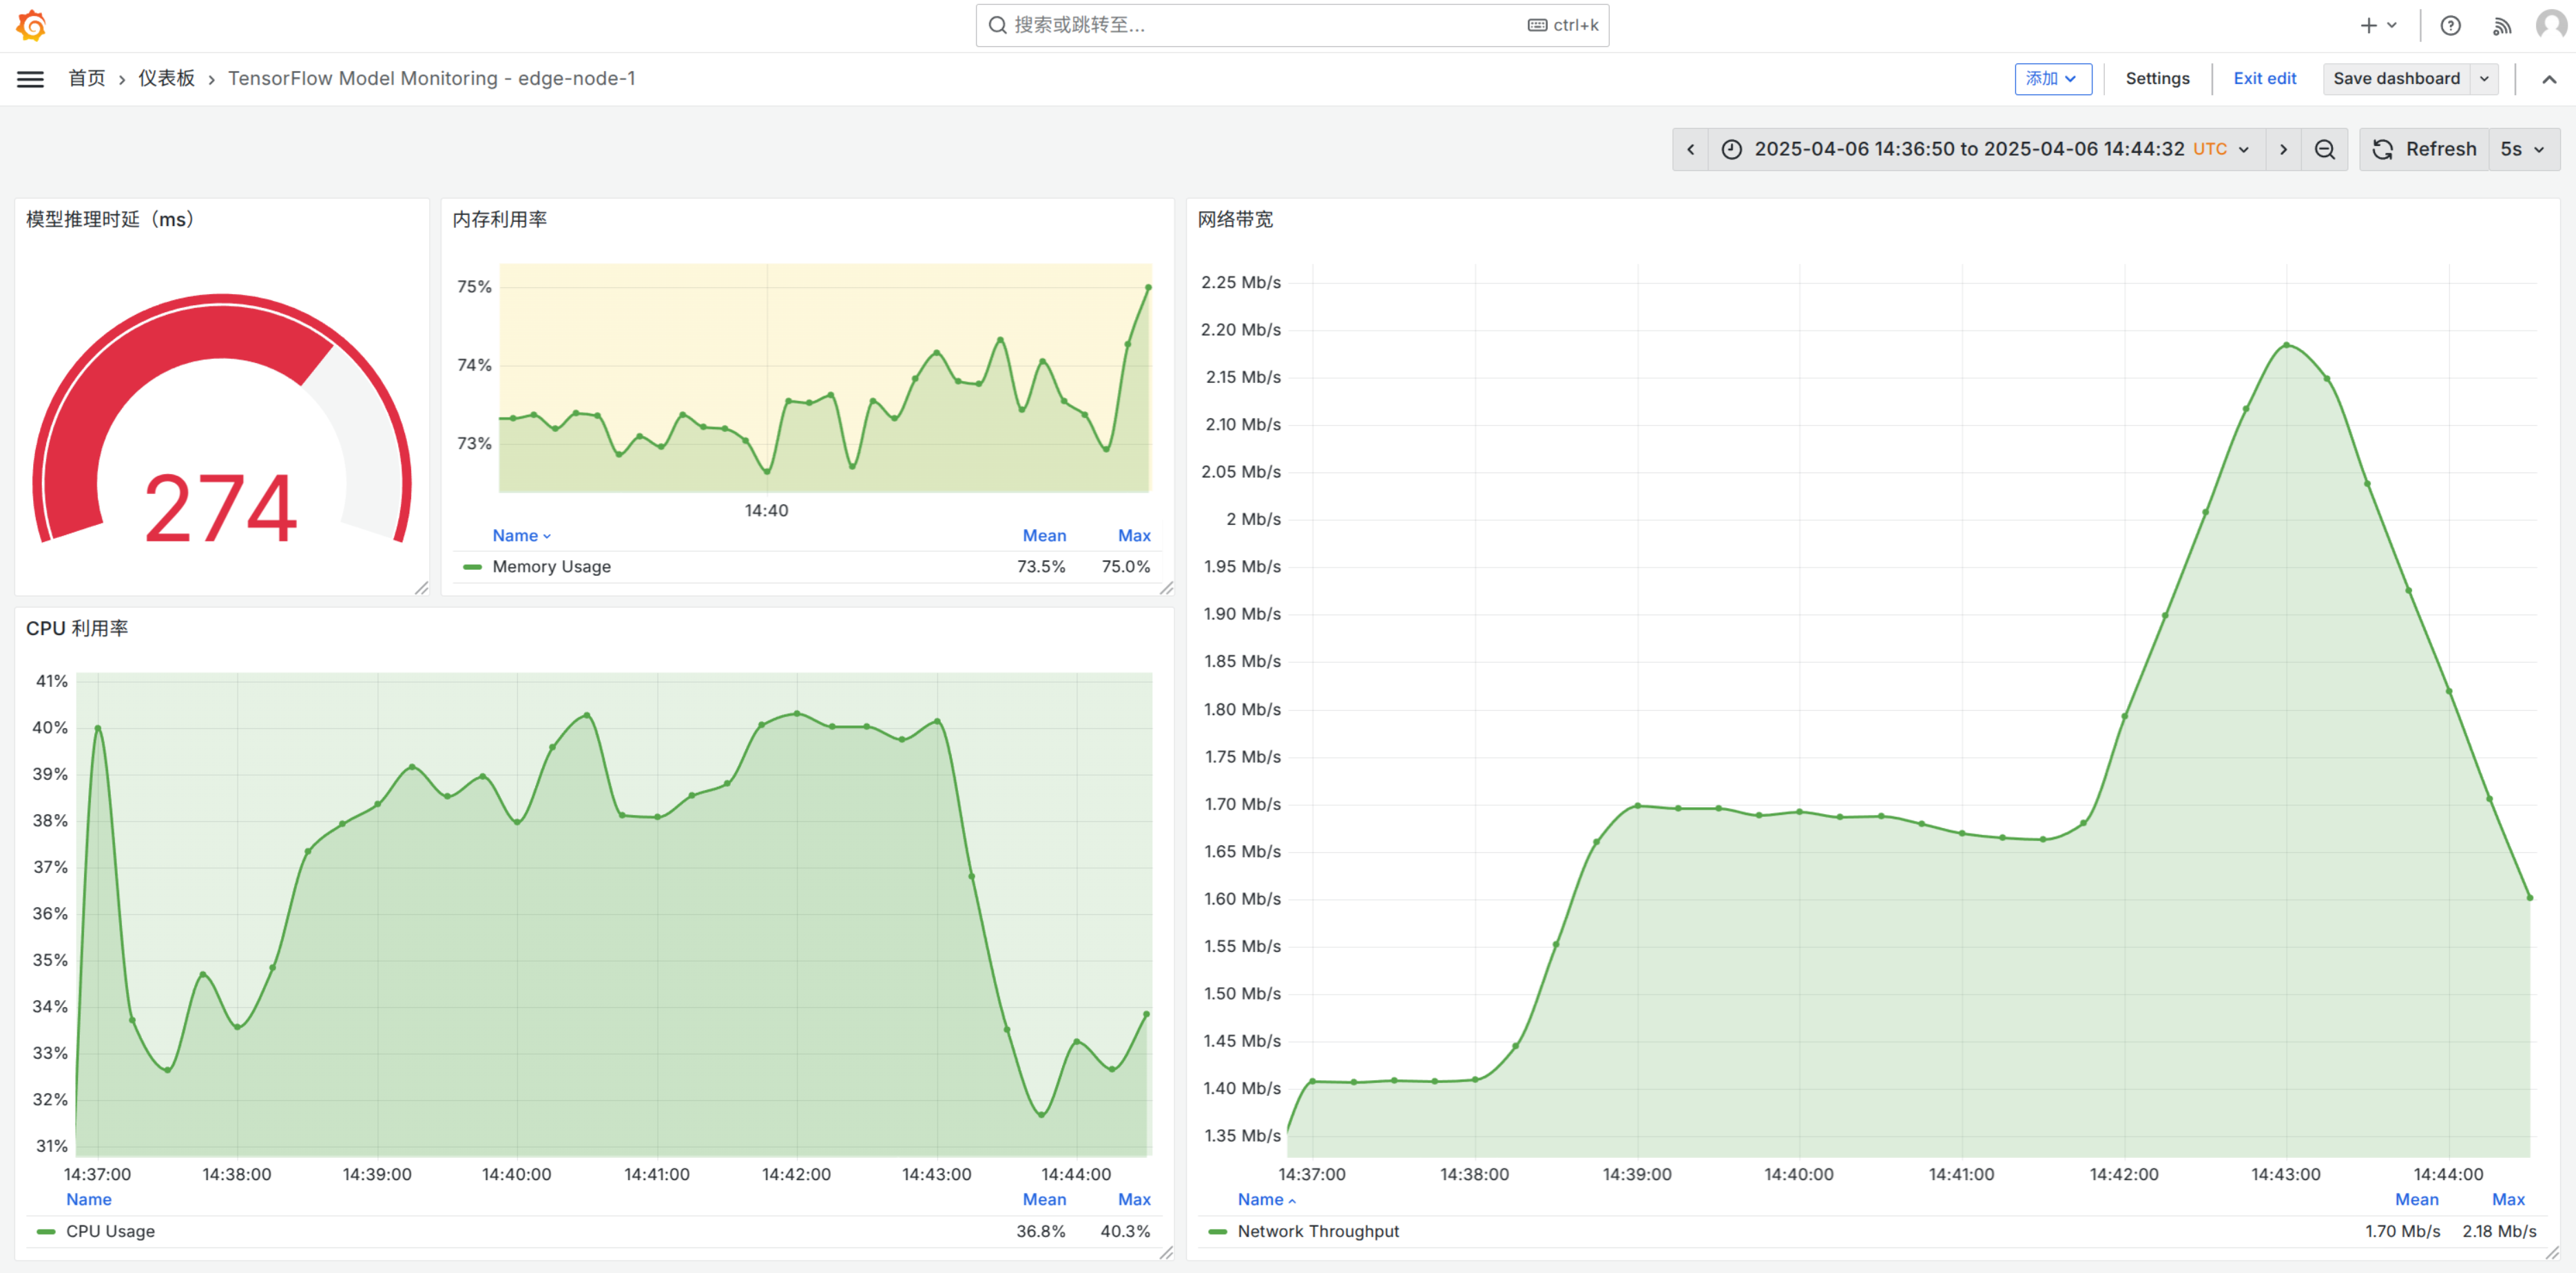
\includegraphics[width=\linewidth]{pics/expr/5-6grafana.png}
  \caption{Grafana 监控仪表盘界面}
  \label{fig:grafana}
\end{figure}

\section{系统性能评估实验}

为了精确衡量调度器的性能,本文在实验中采用了时间戳追踪法。具体而言,在请求生成路由时立即记录第一个时间戳作为等待时间的起点;当系统成功匹配到合适节点并将该请求纳入处理队列时,记录第二个时间戳以标记实际处理开始的时间点;最后,在请求完成全部处理流程后记录第三个时间戳。通过这种方式,可以直接计算出请求在队列中的等待时间和节点实际处理请求所需的时间。

\begin{table}[ht]
    \renewcommand{\arraystretch}{1.5}
    \centering
    \caption{调度器性能评估实验数据}
    \label{tab:performance}
    \begin{tabular}{lll}
        \toprule
        \textbf{平均响应时间} & \textbf{平均等待时间} \\
        \midrule
        $247.29 \, \text{ms}$ & $126.88 \, \text{ms}$  \\ 
        \bottomrule
    \end{tabular}
\end{table}

在上述实验设置下,本文获取了表 \ref{tab:performance} 中的数据,展示了调度器的平均响应时间和平均等待时间。结果显示,调度器表现出较高的处理效率和较低的等待时间,表明其具有良好的性能表现。

\section{本章小结}

本章对 KEAS 方案进行全面实验评估,分为核心算法仿真、系统功能验证和性能评估三部分。核心算法仿真实验通过模拟云边环境中的计算节点与设备流式数据生成过程,验证分层调度优化算法在服务质量指标(如调度成功率)上的表现。系统功能验证实验测试各核心模块的功能完整性,确保其稳定运行与协同能力。系统性能评估实验深入分析了分层调度决策对响应时间的影响。


\chapter{总结与展望}

\section{工作总结}

\section{研究展望}

同一层级计算节点间协作的深度与效率,分布式预处理、模型的分布式训练或推理任务的并行处理,从而提高系统整体性能。



%---------------------------------------------------------------------
%	参考文献
%---------------------------------------------------------------------

% 生成参考文献页
\printbibliography

%---------------------------------------------------------------------
%	致谢
%---------------------------------------------------------------------

\begin{acknowledgement}
  感谢 \href{https://git.nju.edu.cn/nju-lug/lug-introduction}{LUG@NJU}。
\end{acknowledgement}

%---------------------------------------------------------------------
%	学术简历
%---------------------------------------------------------------------

% 详见手册中“成果列表”一节
% \njuchapter{学术成果}
% \njupaperlist[攻读博士学位期间发表的学术论文]{preskill2018}

%---------------------------------------------------------------------
%	附录部分
%---------------------------------------------------------------------

% 附录部分使用单独的字母序号
\appendix

% 可以在这里插入补充材料
\chapter{正文中涉及的数据及源代码}
\dots

% 完工
\end{document}
